\documentclass[11pt]{article}
%DIF LATEXDIFF DIFFERENCE FILE


%%%%%%%%%%%%%%%%%%%%%%%%%%%%%%%%%%%%%%%%%%%%%%%%%%%%%%%%%
%%%%%%%%%%%%%%%%%%%%%%%%% Setup %%%%%%%%%%%%%%%%%%%%%%%%%
\usepackage[margin=1in]{geometry}
\usepackage{fmtcount} % 1st, 2nd...
\usepackage[english]{babel}
\usepackage{soul} % spacing
\usepackage{enumerate} % change enum label
\usepackage{framed} % frame pagebreak
\usepackage{authblk}
\usepackage{setspace}
\usepackage{tocloft}

%%%%% Math, Code 
\usepackage{amsmath}
\usepackage{amsfonts}
\usepackage{amssymb}
\usepackage{amsthm}
\usepackage{amscd}
\usepackage{array}
\usepackage{mathtools} 
\usepackage{verbatim}
\usepackage{fancyvrb} % verbatim
\usepackage{algpseudocode}
\usepackage{algorithm}

%%%%% Graphic, Figure, Table
\usepackage{graphicx}
\usepackage{epstopdf}
\usepackage{xcolor}
\usepackage[labelsep=none]{caption}
\usepackage{subcaption}
\usepackage{multirow} % table
\usepackage{longtable} % table to next page
\usepackage{rotating}
\usepackage{wrapfig} % wrap fig, tbl with text

%%%%% Bib, Cite
\usepackage{url}
\usepackage{cite}
\usepackage{fancyref}
\usepackage{hyperref}
\hypersetup{linktocpage}

%%%%%% Setup
% \captionsetup{compatibility=false} %subfig
% \DeclareCaptionLabelFormat{Sformat}{S#2 #1}
% \captionsetup[figure]{labelformat=Sformat}
% \captionsetup[table]{labelformat=Sformat}
\hypersetup{colorlinks=false}
\setlength{\parskip}{0.5em}

\newtheorem{thm}{Theorem}[section]
\newtheorem{cor}[thm]{Corollary}
\newtheorem{lem}[thm]{Lemma}
\newtheorem{prop}[thm]{Proposition}
\newtheorem{dfn}{Definition}
\newtheorem{ex}{Example}
\newtheorem{cmt}{Cmt}[section]
\newtheorem{rmk}{Remark}[section]
\newcommand{\rb}[1]{\raisebox{-.5em}[0pt]{#1}}
\newcommand{\1}{{\rm 1}\kern-0.24em{\rm I}}
\newcommand{\cN}{\mathcal{N}}
\newcommand{\cO}{\mathcal{O}}
\renewcommand{\mid}{\, | \ , }
\makeatletter
\renewcommand\theequation{S\@arabic\c@equation}
\makeatother

\renewcommand\Affilfont{\normalsize}
% \renewcommand{\baselinestretch}{1.3}

\DeclareMathOperator*{\argmin}{arg\,min}
\DeclareMathOperator*{\argmax}{arg\,max}
\DeclareMathOperator*{\bbr}{\mathbb{R}}
%%%%%%%%%%%%%%%%%%%%%%%%%%%%%%%%%%%%%%%%%%%%%%%%%%%%%%%
%%%%%%%%%%%%%%%%%%%%%%%%%%%%%%%%%%%%%%%%%%%%%%%%%%%%%%%

\title{Supporting Information of ``Multidimensional scaling informed by $F$-statistic: Visualizing grouped microbiome data with inference''}
\author[1\dag]{Hyungseok Kim}
\author[2\dag]{Soobin Kim}
\author[3]{Jeffrey A. Kimbrel}
\author[3]{Megan M. Morris}
\author[3]{Xavier Mayali}
\author[1$*$]{Cullen R. Buie}
\affil[1]{Massachusetts Institute of Technology, Cambridge, MA, USA}
\affil[2]{University of California, Davis, Davis, CA, USA}
\affil[3]{Lawrence Livermore National Laboratory, Livermore, CA, USA}
\affil[$\dagger$] {These authors contributed equally to this work.}
\affil[$^*$]{Correspondence: crb@mit.edu.}
% \author{}
\date{}
%DIF PREAMBLE EXTENSION ADDED BY LATEXDIFF
%DIF UNDERLINE PREAMBLE %DIF PREAMBLE
\RequirePackage[normalem]{ulem} %DIF PREAMBLE
\RequirePackage{color}\definecolor{RED}{rgb}{1,0,0}\definecolor{BLUE}{rgb}{0,0,1} %DIF PREAMBLE
\providecommand{\DIFaddtex}[1]{{\protect\color{blue}\uwave{#1}}} %DIF PREAMBLE
\providecommand{\DIFdeltex}[1]{{\protect\color{red}\sout{#1}}}                      %DIF PREAMBLE
%DIF SAFE PREAMBLE %DIF PREAMBLE
\providecommand{\DIFaddbegin}{} %DIF PREAMBLE
\providecommand{\DIFaddend}{} %DIF PREAMBLE
\providecommand{\DIFdelbegin}{} %DIF PREAMBLE
\providecommand{\DIFdelend}{} %DIF PREAMBLE
\providecommand{\DIFmodbegin}{} %DIF PREAMBLE
\providecommand{\DIFmodend}{} %DIF PREAMBLE
%DIF FLOATSAFE PREAMBLE %DIF PREAMBLE
\providecommand{\DIFaddFL}[1]{\DIFadd{#1}} %DIF PREAMBLE
\providecommand{\DIFdelFL}[1]{\DIFdel{#1}} %DIF PREAMBLE
\providecommand{\DIFaddbeginFL}{} %DIF PREAMBLE
\providecommand{\DIFaddendFL}{} %DIF PREAMBLE
\providecommand{\DIFdelbeginFL}{} %DIF PREAMBLE
\providecommand{\DIFdelendFL}{} %DIF PREAMBLE
%DIF HYPERREF PREAMBLE %DIF PREAMBLE
\providecommand{\DIFadd}[1]{\texorpdfstring{\DIFaddtex{#1}}{#1}} %DIF PREAMBLE
\providecommand{\DIFdel}[1]{\texorpdfstring{\DIFdeltex{#1}}{}} %DIF PREAMBLE
\newcommand{\DIFscaledelfig}{0.5}
%DIF HIGHLIGHTGRAPHICS PREAMBLE %DIF PREAMBLE
\RequirePackage{settobox} %DIF PREAMBLE
\RequirePackage{letltxmacro} %DIF PREAMBLE
\newsavebox{\DIFdelgraphicsbox} %DIF PREAMBLE
\newlength{\DIFdelgraphicswidth} %DIF PREAMBLE
\newlength{\DIFdelgraphicsheight} %DIF PREAMBLE
% store original definition of \includegraphics %DIF PREAMBLE
\LetLtxMacro{\DIFOincludegraphics}{\includegraphics} %DIF PREAMBLE
\newcommand{\DIFaddincludegraphics}[2][]{{\color{blue}\fbox{\DIFOincludegraphics[#1]{#2}}}} %DIF PREAMBLE
\newcommand{\DIFdelincludegraphics}[2][]{% %DIF PREAMBLE
\sbox{\DIFdelgraphicsbox}{\DIFOincludegraphics[#1]{#2}}% %DIF PREAMBLE
\settoboxwidth{\DIFdelgraphicswidth}{\DIFdelgraphicsbox} %DIF PREAMBLE
\settoboxtotalheight{\DIFdelgraphicsheight}{\DIFdelgraphicsbox} %DIF PREAMBLE
\scalebox{\DIFscaledelfig}{% %DIF PREAMBLE
\parbox[b]{\DIFdelgraphicswidth}{\usebox{\DIFdelgraphicsbox}\\[-\baselineskip] \rule{\DIFdelgraphicswidth}{0em}}\llap{\resizebox{\DIFdelgraphicswidth}{\DIFdelgraphicsheight}{% %DIF PREAMBLE
\setlength{\unitlength}{\DIFdelgraphicswidth}% %DIF PREAMBLE
\begin{picture}(1,1)% %DIF PREAMBLE
\thicklines\linethickness{2pt} %DIF PREAMBLE
{\color[rgb]{1,0,0}\put(0,0){\framebox(1,1){}}}% %DIF PREAMBLE
{\color[rgb]{1,0,0}\put(0,0){\line( 1,1){1}}}% %DIF PREAMBLE
{\color[rgb]{1,0,0}\put(0,1){\line(1,-1){1}}}% %DIF PREAMBLE
\end{picture}% %DIF PREAMBLE
}\hspace*{3pt}}} %DIF PREAMBLE
} %DIF PREAMBLE
\LetLtxMacro{\DIFOaddbegin}{\DIFaddbegin} %DIF PREAMBLE
\LetLtxMacro{\DIFOaddend}{\DIFaddend} %DIF PREAMBLE
\LetLtxMacro{\DIFOdelbegin}{\DIFdelbegin} %DIF PREAMBLE
\LetLtxMacro{\DIFOdelend}{\DIFdelend} %DIF PREAMBLE
\DeclareRobustCommand{\DIFaddbegin}{\DIFOaddbegin \let\includegraphics\DIFaddincludegraphics} %DIF PREAMBLE
\DeclareRobustCommand{\DIFaddend}{\DIFOaddend \let\includegraphics\DIFOincludegraphics} %DIF PREAMBLE
\DeclareRobustCommand{\DIFdelbegin}{\DIFOdelbegin \let\includegraphics\DIFdelincludegraphics} %DIF PREAMBLE
\DeclareRobustCommand{\DIFdelend}{\DIFOaddend \let\includegraphics\DIFOincludegraphics} %DIF PREAMBLE
\LetLtxMacro{\DIFOaddbeginFL}{\DIFaddbeginFL} %DIF PREAMBLE
\LetLtxMacro{\DIFOaddendFL}{\DIFaddendFL} %DIF PREAMBLE
\LetLtxMacro{\DIFOdelbeginFL}{\DIFdelbeginFL} %DIF PREAMBLE
\LetLtxMacro{\DIFOdelendFL}{\DIFdelendFL} %DIF PREAMBLE
\DeclareRobustCommand{\DIFaddbeginFL}{\DIFOaddbeginFL \let\includegraphics\DIFaddincludegraphics} %DIF PREAMBLE
\DeclareRobustCommand{\DIFaddendFL}{\DIFOaddendFL \let\includegraphics\DIFOincludegraphics} %DIF PREAMBLE
\DeclareRobustCommand{\DIFdelbeginFL}{\DIFOdelbeginFL \let\includegraphics\DIFdelincludegraphics} %DIF PREAMBLE
\DeclareRobustCommand{\DIFdelendFL}{\DIFOaddendFL \let\includegraphics\DIFOincludegraphics} %DIF PREAMBLE
%DIF END PREAMBLE EXTENSION ADDED BY LATEXDIFF

\begin{document}

\renewcommand*\contentsname{\normalsize List of Supplementary Notes}
\makeatletter
\renewcommand{\tableofcontents}{\@starttoc{toc}}
\renewcommand*\l@section{\@dottedtocline{1}{0em}{6.3em}}
\let\l@table\l@content
\makeatother

\makeatletter
\renewcommand{\listoffigures}{\@starttoc{lof}}
\renewcommand*\l@figure{\@dottedtocline{1}{0em}{3.5em}}
\let\l@table\l@figure
\makeatother

\makeatletter
\renewcommand{\listoftables}{\@starttoc{lot}}
\renewcommand*\l@table{\@dottedtocline{1}{0em}{4.5em}}
\let\l@table\l@table
\makeatother

\renewcommand\thesection{S\arabic{section} Appendix.}
\makeatletter
\renewcommand*{\@seccntformat}[1]{\csname the#1\endcsname\hspace{0.5em}}
\makeatother

\renewcommand{\figurename}{\!\!}
\let\standardthefigure\thefigure
\renewcommand\thefigure{S\standardthefigure\ Fig.\ }
\addtolength{\cftfignumwidth}{15pt}

\renewcommand{\tablename}{\!\!}
\let\standardthetable\thetable
\renewcommand\thetable{S\standardthetable\ Table.\ }

% \renewcommand{\algorithmname}{\!\!}
\let\standardthealgorithm\thealgorithm
\renewcommand\thealgorithm{S\standardthealgorithm}

\maketitle
% \def\thefootnote{\arabic{footnote}}

{\noindent\normalsize\bf List of Supplementary Information}
\tableofcontents
\listoffigures
\listoftables
\clearpage


\section{\DIFdelbegin \DIFdel{Mapping }\DIFdelend \DIFaddbegin \DIFadd{Objective }\DIFaddend function for \DIFaddbegin \DIFadd{computing }\DIFaddend $F$-MDS\DIFdelbegin \DIFdel{.}\DIFdelend } \label{sec:app1}

\DIFdelbegin \DIFdel{In this section, we explain a procedure of deriving a }\DIFdelend \DIFaddbegin \DIFadd{First, we derive a }\DIFaddend mapping function $f_\mathbf{z}(F_\mathbf{x})$ \DIFdelbegin \DIFdel{that is used to minimize }\DIFdelend \DIFaddbegin \DIFadd{for minimizing }\DIFaddend an objective function \DIFdelbegin \DIFdel{for }\DIFdelend \DIFaddbegin \DIFadd{and }\DIFaddend computing $F$-informed MDS.
The \DIFdelbegin \DIFdel{confirmatory term of the objective function (Eq 5 of the main text) is specifically designed }\DIFdelend \DIFaddbegin \DIFadd{mapping function guides }\DIFaddend to minimize a difference in $p$-values testing \DIFdelbegin \DIFdel{for group difference by representations }\DIFdelend \DIFaddbegin \DIFadd{group differences }\DIFaddend under the original $S$- and \DIFdelbegin \DIFdel{two-dimensions}\DIFdelend \DIFaddbegin \DIFadd{two-dimensional embedding through the confirmatory term of the objective (see Eq 5 of the main text)}\DIFaddend .
These \textit{p}-values are obtained from an empirical distribution of the pseudo-$F$s by permuted labels \cite{anderson01} \DIFdelbegin \DIFdel{. 
In other words, by denoting a label set as $[y_i]$ ($i=1,\cdots N$) and its permuted set as $[y_i^\pi]$ with operator $\pi$, we express each }\DIFdelend \DIFaddbegin \DIFadd{(Eq 4, main text). 
For a given label set $[y_i]_{i=1}^{N}$ and its group number $G$, a permuted label set $[y_i^\Pi]_{i=1}^{N}$ and }\DIFaddend $F$\DIFdelbegin \DIFdel{-statistic as
}\DIFdelend \DIFaddbegin \DIFadd{-statistics are expressed as
}\DIFaddend \begin{equation}
\DIFdelbegin %DIFDELCMD < \begin{aligned}
%DIFDELCMD < F^\pi_\mathbf{x} &= 
%DIFDELCMD < \left(\frac{\sum_{i,j}d_{ij}^2}{2\sum_{i,j}d_{ij}^2\,\1\{y_i^\pi = y_j^\pi\}} -1 \right) \cdot (N-2), \\
%DIFDELCMD < F^\pi_\mathbf{z} &= 
%DIFDELCMD < \left(\frac{\sum_{i,j}\|\mathbf{z}_i - \mathbf{z}_j\|_2^2}{2\sum_{i,j}\|\mathbf{z}_i - \mathbf{z}_j\|_2^2\,\1\{y_i^\pi = y_j^\pi\}} -1 \right) \cdot (N-2).
%DIFDELCMD < \label{eq:map1}
%DIFDELCMD < \end{aligned}%%%
\DIFdelend \DIFaddbegin \begin{aligned}
F^\Pi_\mathbf{x} &= 
\left(\frac{\sum_{i,j}d_{ij}^2}{G \sum_{i,j}d_{ij}^2\,\1\{y_i^\Pi = y_j^\Pi\}} -1 \right) \cdot \frac{N-G}{G-1}, \\
F^\Pi_\mathbf{z} &= 
\left(\frac{\sum_{i,j}\|\mathbf{z}_i - \mathbf{z}_j\|_2^2}{G\sum_{i,j}\|\mathbf{z}_i - \mathbf{z}_j\|_2^2\,\1\{y_i^\Pi = y_j^\Pi\}} -1 \right) \cdot \frac{N-G}{G-1}.
\label{eq:map1}
\end{aligned}\DIFaddend 
\end{equation}
% \end{align} 

It should be noted that the pseudo $F$-ratios can range differently based on how the samples are projected onto 2D. To scale between these two ratios and minimize the difference in $p$-values, we consider a mapping $f_\mathbf{z}: F_\mathbf{x} \rightarrow F_\mathbf{z}$ from a pair of ratios \DIFdelbegin \DIFdel{$(F_\mathbf{x}^{\pi_1}, F_\mathbf{z}^{\pi_2})$ }\DIFdelend \DIFaddbegin \DIFadd{$(F_\mathbf{x}^{\Pi_1}, F_\mathbf{z}^{\Pi_2})$ }\DIFaddend where each element was ordered from two independent sets of repeated permutations. Figure below exemplifies how the $F$-ratios at each dimensionality scaled differently and depended on the choice of hyperparameter $\lambda$. In both settings, the $F$-ratio in $S$-dimension ranged \DIFdelbegin \DIFdel{between zero and six }\DIFdelend \DIFaddbegin \DIFadd{in }[\DIFadd{0,6}] \DIFaddend whereas in 2D representation the ratio ranged in [0,4]. The hyperparameter, however, impacted the detailed relationship between ordered $F_\mathbf{x}$ and ordered $F_\mathbf{x}$, when compared to each other. 

\begin{figure}[h]
    \centering
    \includegraphics[width=5.5in]{submissions/plos/figures/supp-mds_Fval.pdf}
    \caption*{Figure: Mapping pseudo-$F$'s between two dimensionalities. Each $F_\mathbf{x} \text{-} F_\mathbf{z}$ relationship was obtained by permuting labels over 1,000 times, and by setting a hyperparameter $\lambda$ that is used to perform the majorization.}
    \label{fig:mds-fval}
\end{figure}

Using the mapping function $f_\mathbf{z}$, we \DIFdelbegin \DIFdel{now }\DIFdelend derive an exact \DIFdelbegin \DIFdel{form of confirmatory term proposed }\DIFdelend \DIFaddbegin \DIFadd{expression for the confirmatory term introduced }\DIFaddend in the $F$-MDS objective function\DIFdelbegin \DIFdel{(Eq 5 of main text)}\DIFdelend . The proposed form $\left|F_\mathbf{z} - f_\mathbf{z}(F_\mathbf{x})\right|$ measures how \DIFaddbegin \DIFadd{accurately }\DIFaddend the 2D representation \DIFdelbegin \DIFdel{accurately reflected }\DIFdelend \DIFaddbegin \DIFadd{reflects }\DIFaddend the $S$-dimensional distance structure \DIFdelbegin \DIFdel{with respect to }\DIFdelend \DIFaddbegin \DIFadd{regarding }\DIFaddend the sample labels. \DIFdelbegin \DIFdel{Having the }\DIFdelend \DIFaddbegin \DIFadd{A }\DIFaddend difference close to zero indicates that no \DIFdelbegin \DIFdel{additional update with the representation is required (let us denote it as }\DIFdelend \DIFaddbegin \DIFadd{further updates to the representation are required (denoted }\DIFaddend $\mathbf{Z}^*$). \DIFdelbegin \DIFdel{Now by substituting }\DIFdelend \DIFaddbegin \DIFadd{Substituting }\DIFaddend the confirmatory term $\left|F_\mathbf{z} - f_\mathbf{z}(F_\mathbf{x})\right|$ with Equation \ref{eq:map1}, we define \DIFdelbegin \DIFdel{$\1\{y_i^\pi = y_j^\pi\}\coloneqq\epsilon_{ij}$ and write
}\DIFdelend \DIFaddbegin \DIFadd{$\epsilon_{ij}\coloneqq\1\{y_i^\Pi = y_j^\Pi\}$ and write
}\DIFaddend \begin{align}
\mathbf{Z}^* &= \argmin_\mathbf{Z}\,\left|F_\mathbf{z} - f_\mathbf{z}(F_\mathbf{x})\right| \\
& = \argmin_\mathbf{Z}\,\left|\DIFdelbegin \DIFdel{(N-2)}\DIFdelend \DIFaddbegin \DIFadd{\frac{N-G}{G-1}}\DIFaddend \cdot\left(\DIFdelbegin \DIFdel{\frac{\sum_{i,j}\|\mathbf{z}_i - \mathbf{z}_j\|_2^2}{2\sum_{i,j}\epsilon_{ij}\|\mathbf{z}_i - \mathbf{z}_j\|_2^2} }\DIFdelend \DIFaddbegin \DIFadd{\frac{\sum_{i,j}\|\mathbf{z}_i - \mathbf{z}_j\|_2^2}{G\sum_{i,j}\epsilon_{ij}\|\mathbf{z}_i - \mathbf{z}_j\|_2^2} }\DIFaddend -1 \right) - f_\mathbf{z}(F_\mathbf{x})\right| \\
&= \argmin_\mathbf{Z}\,\left|\DIFdelbegin \DIFdel{\frac{\sum_{i,j}\|\mathbf{z}_i - \mathbf{z}_j\|_2^2}{2\sum_{i,j}\epsilon_{ij}\|\mathbf{z}_i - \mathbf{z}_j\|_2^2} }\DIFdelend \DIFaddbegin \DIFadd{\frac{\sum_{i,j}\|\mathbf{z}_i - \mathbf{z}_j\|_2^2}{G\sum_{i,j}\epsilon_{ij}\|\mathbf{z}_i - \mathbf{z}_j\|_2^2} }\DIFaddend -1 - \DIFdelbegin \DIFdel{\frac{f_\mathbf{z}(F_\mathbf{x})}{N-2} }\DIFdelend \DIFaddbegin \DIFadd{\frac{G-1}{N-G}\cdot{f_\mathbf{z}(F_\mathbf{x})} }\DIFaddend \right| \DIFdelbegin %DIFDELCMD < \\
%DIFDELCMD < &%%%
\DIFdel{= \argmin_\mathbf{Z}\,}%DIFDELCMD < \left| %%%
\DIFdel{\frac{\sum_{i,j}\|\mathbf{z}_i - \mathbf{z}_j\|_2^2 - 2\sum_{i,j}\epsilon_{ij}\|\mathbf{z}_i - \mathbf{z}_j\|_2^2 \cdot [1+f_\mathbf{z}(F_\mathbf{x})/(N-2)]}{2\sum_{i,j}\epsilon_{ij}\|\mathbf{z}_i - \mathbf{z}_j\|_2^2} }%DIFDELCMD < \right| %%%
\DIFdelend \label{eq:pre_approx}\\
&\approx \argmin_\mathbf{Z}\,\left| \sum_{i,j}\|\mathbf{z}_i - \mathbf{z}_j\|_2^2 - \DIFdelbegin \DIFdel{2}\DIFdelend \DIFaddbegin \DIFadd{G}\DIFaddend \sum_{i,j}\epsilon_{ij}\|\mathbf{z}_i - \mathbf{z}_j\|_2^2 \cdot \left(1+\DIFdelbegin \DIFdel{\frac{f_\mathbf{z}(F_\mathbf{x})}{N-2}}\DIFdelend \DIFaddbegin \DIFadd{\frac{G-1}{N-G}\cdot{f_\mathbf{z}(F_\mathbf{x})}}\DIFaddend \right) \right| \label{eq:approx}\\
&= \argmin_\mathbf{Z}\,\left|\sum_{i,j} \left[1- \DIFdelbegin \DIFdel{2}\DIFdelend \DIFaddbegin \DIFadd{G}\DIFaddend \epsilon_{ij} \left(1+\DIFdelbegin \DIFdel{\frac{f_\mathbf{z}(F_\mathbf{x})}{N-2}}\DIFdelend \DIFaddbegin \DIFadd{\frac{G-1}{N-G}\cdot{f_\mathbf{z}(F_\mathbf{x})}}\DIFaddend \right)\right] \|\mathbf{z}_i - \mathbf{z}_j\|_2^2\right| \DIFaddbegin \label{eq:pre_conf}\DIFaddend ,
\end{align}
where Equation \ref{eq:approx} \DIFdelbegin \DIFdel{is approximated from Equation \ref{eq:pre_approx} }\DIFdelend \DIFaddbegin \DIFadd{follows from the numerator of Equation \ref{eq:pre_approx}. 
}

\DIFadd{Finally, the exact $F$-MDS confirmatory term is derived through a scaling analysis of expression \ref{eq:pre_conf} by comparing its value to that of the raw stress (main text Eq 1). Binary semisynthetic datasets generated by SparseDOSSA \mbox{%DIFAUXCMD
\cite{Ma21}}\hskip0pt%DIFAUXCMD
, with sizes $N$ varying from 50 }\DIFaddend to \DIFdelbegin \DIFdel{ensure that the same physical dimension as the stress term was obtained.
By substituting expression in Equation \ref{eq:pre_approx} with the proposed confirmatory term}\DIFdelend \DIFaddbegin \DIFadd{1000, were used to compute the following quantities,
}\begin{align}
\DIFadd{\text{Raw stress} }&\DIFadd{= \sum_{i,j} (d_{ij} - \| \mathbf{z}_i - \mathbf{z}_j \|_2 )^2 }\\
\DIFadd{\text{Pre-confirmatory} }&\DIFadd{= \sum_{i,j} \left[1- G\epsilon_{ij} \left(1+\frac{G-1}{N-G}\cdot{f_\mathbf{z}(F_\mathbf{x})}\right)\right] \|\mathbf{z}_i - \mathbf{z}_j\|_2^2.
}\end{align}
\begin{figure}[h]
    \centering
    \includegraphics[width=6.5in]{submissions/plos/figures/supp-scaling.pdf}
    \caption*{Figure: Scaling analysis of raw stress and pre-confirmatory terms across data size $N\in\{50,100,200,500,1000\}$ with semisynthetic data.}
    \label{fig:supp_scaling}
\end{figure}
\DIFadd{Computing these two values across different data sizes $N$, as shown in the figure above, indicates that the raw stress and pre-confirmatory terms scale differentially with $N$, with approximate powers 2.1 and 1.0, respectively. While the theoretical foundations remain to be established for such zero-inflated}\DIFaddend , \DIFaddbegin \DIFadd{log-normally distributed data, empirical analysis suggests that the size effect can be removed by multiplying the pre-confirmatory term with $N$.
}

\DIFadd{By combining raw stress and confirmatory terms with hyperparameter $\lambda$, }\DIFaddend we conclude \DIFdelbegin \DIFdel{by deriving the exact form }\DIFdelend \DIFaddbegin \DIFadd{the derivation }\DIFaddend of the $F$-MDS objective \DIFdelbegin \DIFdel{as
}\DIFdelend \DIFaddbegin \DIFadd{function as
}\DIFaddend \begin{equation}
    O_{\rm FMDS}(\mathbf{Z}) = \sum_{i,j} (d_{ij} - \| \mathbf{z}_i - \mathbf{z}_j \|_2 )^2 + \lambda \DIFaddbegin \DIFadd{N }\DIFaddend \left|\sum_{i,j} \left[1- \DIFdelbegin \DIFdel{2}\DIFdelend \DIFaddbegin \DIFadd{G}\DIFaddend \epsilon_{ij} \left(1+\DIFdelbegin \DIFdel{\frac{f_\mathbf{z}(F_\mathbf{x})}{N-2}}\DIFdelend \DIFaddbegin \DIFadd{\frac{G-1}{N-G}\cdot{f_\mathbf{z}(F_\mathbf{x})}}\DIFaddend \right)\right] \|\mathbf{z}_i - \mathbf{z}_j\|_2^2\right|.
\label{eq:fmds_objective}
\end{equation}



\section{Majorization algorithm\DIFdelbegin \DIFdel{.}\DIFdelend } \label{sec:app2}

We seek a configuration $\mathbf{Z^*}= (\mathbf{z}_1^*, \cdots \mathbf{z}_N^*)\in \bbr^{N\times 2}$ that minimizes \DIFdelbegin \DIFdel{an objective term for }\DIFdelend \DIFaddbegin \DIFadd{the }\DIFaddend $F$-MDS \DIFaddbegin \DIFadd{objective function}\DIFaddend , $O_{\text{FMDS}}(\mathbf{Z})$\DIFdelbegin \DIFdel{(Equation \ref{eq:fmds_objective})}\DIFdelend .
Previous work by Witten \& Tibshirani \cite{witten11} suggests that MDS-based ordinations can be computed by applying the Majorization (or Majorize-Minimization) algorithm \DIFdelbegin \DIFdel{where }\DIFdelend to a quadratic expression in \DIFdelbegin \DIFdel{terms of }\DIFdelend $\mathbf{Z}$\DIFdelbegin \DIFdel{is analytically solved. }\DIFdelend \DIFaddbegin \DIFadd{. 
Although our $F$-MDS objective function is also quadratic in $\mathbf{Z}$ and the Majorization algorithm is applicable, the coefficient of the confirmatory term depends on the sample size $N$ and the hyperparameter $\lambda$, as shown in Equation \ref{eq:fmds_objective}.
For the algorithm to consistently produce the optimized $\mathbf{Z}$, it is important to define an update rule that is independent of the sample size. Therefore, we exclude the coefficient $N$ from Equation \ref{eq:fmds_objective}, and to further ensure the convexity of the majorized form, we constrain $\lambda$ to }[\DIFadd{0,1}]\DIFadd{:
}\begin{align*}
\DIFadd{\text{minimize } O^* (\mathbf{Z}) = \sum_{i,j} (d_{ij} - \| \mathbf{z}_i - \mathbf{z}_j \|_2 )^2 + \lambda \left|\sum_{i,j} \left[1- G\epsilon_{ij} \left(1+\frac{G-1}{N-G}\cdot{f_\mathbf{z}(F_\mathbf{x})}\right)\right] \|\mathbf{z}_i - \mathbf{z}_j\|_2^2\right|.
}\end{align*}

\DIFaddend In detail, \DIFaddbegin \DIFadd{the algorithm sequentially seeks a point $\mathbf{z}_k^*$ }\DIFaddend for every $k=1,\cdots N$, \DIFdelbegin \DIFdel{a point $\mathbf{z}_k^*$ minimizing $O_{\text{FMDS}}(\mathbf{Z})$, }\DIFdelend while other configuration points \DIFdelbegin \DIFdel{fixed, }\DIFdelend \DIFaddbegin \DIFadd{remain fixed. This }\DIFaddend is written as
\begingroup
\allowdisplaybreaks
\begin{align}
\mathbf{z}_k^* 
&= \argmin_{\mathbf{z}_k}O\DIFdelbegin \DIFdel{_{\rm FMDS}}\DIFdelend \DIFaddbegin \DIFadd{^*}\DIFaddend (\mathbf{Z} | \mathbf{z}_1,\cdots \mathbf{z}_{k-1}, \mathbf{z}_{k+1}, \mathbf{z}_N) \\
&= \argmin_{\mathbf{z}_k}\, \sum\DIFdelbegin \DIFdel{_{i,j} (d_{ij} - \|\mathbf{z}_i - \mathbf{z}_j\|_2)^2 + \lambda}%DIFDELCMD < \left|%%%
\DIFdel{\sum_{i,j} }%DIFDELCMD < \left[%%%
\DIFdel{1- 2\epsilon_{ij} }%DIFDELCMD < \left(%%%
\DIFdel{1+\frac{f_\mathbf{z}(F)}{N-2}}%DIFDELCMD < \right)\right] %%%
\DIFdel{\|\mathbf{z}_i - \mathbf{z}_j\|_2^2}%DIFDELCMD < \right| \\
%DIFDELCMD < &%%%
\DIFdel{= \argmin_{\mathbf{z}_k}\, \sum}\DIFdelend _{j=1}^N (d_{jk} - \|\mathbf{z}_j - \mathbf{z}_k\|_2)^2 + \lambda\delta(\mathbf{z})\sum_{j=1}^N \left[1- \DIFdelbegin \DIFdel{2}\DIFdelend \DIFaddbegin \DIFadd{G}\DIFaddend \epsilon_{jk} \left(1 + \DIFdelbegin \DIFdel{\frac{f_\mathbf{z}(F)}{N-2}}\DIFdelend \DIFaddbegin \DIFadd{\frac{G-1}{N-G}{f_\mathbf{z}(F)}}\DIFaddend \right)\right] \DIFdelbegin \DIFdel{\cdot }\DIFdelend \|\mathbf{z}_j - \mathbf{z}_k\|_2^2 \\
&= \argmin_{\mathbf{z}_k}\, \sum_{j=1}^N \left[1+\lambda\delta(\mathbf{z}) \left(1- \DIFdelbegin \DIFdel{2}\DIFdelend \DIFaddbegin \DIFadd{G}\DIFaddend \epsilon_{jk} \left(1+ \DIFdelbegin \DIFdel{\frac{f_\mathbf{z}(F)}{N-2}}\DIFdelend \DIFaddbegin \DIFadd{\frac{G-1}{N-G}{f_\mathbf{z}(F)} }\DIFaddend \right)\right) \right] \|\mathbf{z}_k-\mathbf{z}_j\|_2^2 - 2d_{jk}\|\mathbf{z}_k-\mathbf{z}_j\|_2
\label{eq:appc_mm1}
\end{align}
\endgroup
where we \DIFdelbegin \DIFdel{have defined $\delta (\mathbf{z})$ as
}\begin{align*}
\DIFdel{\delta (\mathbf{z}) = \text{sign}\left\{\,\sum_{i,j} \left[1- 2\epsilon_{ij} \left(1+\frac{f_\mathbf{z}(F)}{N-2}\right)\right] \|\mathbf{z}_i - \mathbf{z}_j\|_2^2\right\}.
}\end{align*}%DIFAUXCMD
\DIFdelend \DIFaddbegin \DIFadd{define $\delta (\mathbf{z}) \coloneqq \text{sign}\left\{\,\sum_{i,j} \left[1- G \epsilon_{ij} \left(1 + \frac{G-1}{N-G}{f_\mathbf{z}(F)} \right)\right] \|\mathbf{z}_i - \mathbf{z}_j\|_2^2\right\}$.
}\DIFaddend 

As described by \cite{borg97b}, applying the algorithm starts with majorizing with Equation \ref{eq:appc_mm1},
\begin{equation}
\sum_{j=1}^N\,
\left[1+\lambda\delta(\mathbf{z}) \left(1- \DIFdelbegin \DIFdel{2}\DIFdelend \DIFaddbegin \DIFadd{G }\DIFaddend \epsilon_{jk} \left(1+ \DIFdelbegin \DIFdel{\frac{f_\mathbf{z}(F)}{N-2}}\DIFdelend \DIFaddbegin \DIFadd{\frac{G-1}{N-G}{f_\mathbf{z}(F)} }\DIFaddend \right)\right) \right] \|\mathbf{z}_k-\mathbf{z}_j\|_2^2 - 2d_{jk}\,\frac{\sum_{s=1}^2 (z_{ks}-z_{js})(\Tilde{z}_{ks}-z_{js})}{\|\Tilde{\mathbf{z}}_k-\mathbf{z}_j\|_2}, \label{eq:appc_mm2}
\end{equation}
where $\Tilde{\mathbf{z}}_k$ \DIFdelbegin \DIFdel{is a fixed term (not updated) while }\DIFdelend \DIFaddbegin \DIFadd{remain fixed while updating }\DIFaddend ${\mathbf{z}}_k$\DIFdelbegin \DIFdel{still remains as a variable}\DIFdelend . We further assume that a change of mapping function $f_\mathbf{z}(F)$ is negligible and that $\delta(\mathbf{z})$ remains constant during the iteration (e.g., a small change in $\mathbf{z}_k$ from metric MDS). These allow us to approximate Equation \ref{eq:appc_mm2} with a quadratic expression in terms of $\mathbf{z}$ and proceed to its minimization\DIFdelbegin \DIFdel{analytically}\DIFdelend \DIFaddbegin \DIFadd{, given its convexity}\DIFaddend .
To find \DIFdelbegin \DIFdel{its }\DIFdelend \DIFaddbegin \DIFadd{the }\DIFaddend minimum at $\mathbf{z}_{k}=\mathbf{z}_{k}^\dagger$, a derivative is taken with respect to $z_{ks}$ and is set to zero.
\DIFdelbegin \DIFdel{In other words, we obtain
}\DIFdelend \DIFaddbegin \DIFadd{Applying it to Equation \ref{eq:appc_mm2}, we have
}\DIFaddend \begin{align}
\begin{split}
0 = \sum_{j=1}^N\, \left[1+\lambda\delta(\mathbf{z}) \left(1- \DIFdelbegin \DIFdel{2}\DIFdelend \DIFaddbegin \DIFadd{G}\DIFaddend \epsilon_{jk} \left(1 + \DIFdelbegin \DIFdel{\frac{f_\mathbf{z}(F)}{N-2}}\DIFdelend \DIFaddbegin \DIFadd{\frac{G-1}{N-G}{f_\mathbf{z}(F)} }\DIFaddend \right)\right) \right] (z_{ks}^\dagger - z_{js}) 
- d_{jk}\frac{\Tilde{z}_{ks}-z_{js}}{\|\Tilde{\mathbf{z}}_k-\mathbf{z}_j\|_2}\DIFdelbegin \DIFdel{.
}\DIFdelend \DIFaddbegin \DIFadd{, \forall s=1,2
}\DIFaddend \label{eq:mm_balance}
\end{split}
\end{align}
\DIFdelbegin %DIFDELCMD < 

%DIFDELCMD < %%%
\DIFdel{Noting that }\DIFdelend \DIFaddbegin \DIFadd{and }\DIFaddend for a balanced design where \DIFdelbegin \DIFdel{$\sum_{j=1}^N \epsilon_{jk}= {N}/{2}$, for }\DIFdelend \DIFaddbegin \DIFadd{$\sum_{j=1}^N \epsilon_{jk}= {N}/{G}$ with every }\DIFaddend $k=1,\cdots N$,
\DIFdelbegin \DIFdel{we rewrite Equation \ref{eq:mm_balance} and analytically obtain $z_{ks}^\dagger$:
}\DIFdelend \begin{align}
\DIFdelbegin %DIFDELCMD < \begin{split}
%DIFDELCMD < & %%%
\DIFdel{\sum_{j=1}^N\, }%DIFDELCMD < \left[%%%
\DIFdel{1+\lambda\delta(\mathbf{z}) }\DIFdelend \left( \DIFdelbegin \DIFdel{1- 2\epsilon_{jk} }%DIFDELCMD < \left(%%%
\DIFdel{1+\frac{f_\mathbf{z}(F)}{N-2}}%DIFDELCMD < \right)\right) \right] %%%
\DIFdel{z_{ks}^\dagger 
= }%DIFDELCMD < \left( %%%
\DIFdelend N - \DIFdelbegin \DIFdel{\frac{N\lambda\delta(\mathbf{z})f_\mathbf{z}(F)}{N-2} }\DIFdelend \DIFaddbegin \DIFadd{\frac{(G-1)N\lambda\delta(\mathbf{z})f_\mathbf{z}(F)}{N-G} }\DIFaddend \right) z_{ks}^\dagger \DIFdelbegin %DIFDELCMD < \\
%DIFDELCMD < &%%%
\DIFdel{\qquad}\DIFdelend = \sum_{j=1}^N\, \left[1+\lambda\delta(\mathbf{z}) \left(1- \DIFdelbegin \DIFdel{2}\DIFdelend \DIFaddbegin \DIFadd{G }\DIFaddend \epsilon_{jk} \left(1+ \DIFdelbegin \DIFdel{\frac{f_\mathbf{z}(F)}{N-2}}\DIFdelend \DIFaddbegin \DIFadd{\frac{G-1}{N-G}{f_\mathbf{z}(F)} }\DIFaddend \right)\right) \right] z_{js} + d_{jk}\frac{\Tilde{z}_{ks}-z_{js}}{\|\Tilde{\mathbf{z}}_k-\mathbf{z}_j\|_2}.
\DIFdelbegin %DIFDELCMD < \end{split}
%DIFDELCMD < %%%
\DIFdelend \DIFaddbegin \label{eq:update_element}
\DIFaddend \end{align}
\DIFdelbegin \begin{align*}
\begin{split}
\DIFdel{\therefore z_{ks}^\dagger = 
}&\DIFdel{\frac{(N-2)}{N(N-2) - N\lambda\delta(\mathbf{z}) f_\mathbf{z}(F)} }\\
&\DIFdel{\quad\times\left\{\sum_{j=1}^N\, \left[1+\lambda\delta(\mathbf{z}) \left(1- 2\epsilon_{jk} \left(1+\frac{f_\mathbf{z}(F)}{N-2}\right)\right) \right]  z_{js} + d_{jk}\frac{\Tilde{z}_{ks}-z_{js}}{\|\Tilde{\mathbf{z}}_k-\mathbf{z}_j\|_2}\right\}.
\label{eq:update_element}
}\end{split}
\DIFdel{}\end{align*}%DIFAUXCMD
\DIFdel{Finally, rewriting }\DIFdelend \DIFaddbegin \DIFadd{Rewriting }\DIFaddend Equation \ref{eq:update_element} in a vector form\DIFdelbegin \DIFdel{gives us an }\DIFdelend \DIFaddbegin \DIFadd{, we finally obtain the }\DIFaddend update rule of $\mathbf{Z}$ as
\DIFdelbegin \DIFdel{below:
}\DIFdelend 
\begin{align}
\begin{split}
\mathbf{z}_k \gets
\DIFdelbegin \DIFdel{\frac{(N-2)}{N(N-2) - N\lambda\delta(\mathbf{z}) f_\mathbf{z}(F)}\cdot }\DIFdelend \DIFaddbegin & \DIFadd{\frac{N-G}{N(N-G) - (G-1)N\lambda\delta(\mathbf{z}) f_\mathbf{z}(F)}\times }\\ 
&\DIFadd{\quad}\DIFaddend \left\{\sum_{j=1}^N\, \left[1+\lambda\delta(\mathbf{z}) \left(1- \DIFdelbegin \DIFdel{2}\DIFdelend \DIFaddbegin \DIFadd{G }\DIFaddend \epsilon_{jk} \left(1+ \DIFdelbegin \DIFdel{\frac{f_\mathbf{z}(F)}{N-2}}\DIFdelend \DIFaddbegin \DIFadd{\frac{G-1}{N-G}{f_\mathbf{z}(F)} }\DIFaddend \right)\right) \right]  \mathbf{z}_{j} + d_{jk}\frac{\mathbf{z}_k -\mathbf{z}_j}{\|{\mathbf{z}}_k-\mathbf{z}_j\|_2}\right\}.
% \label{eq:mm_update}
\end{split}
\end{align}



\section{\DIFdelbegin \DIFdel{Human gut microbiome dataset.}\DIFdelend \DIFaddbegin \DIFadd{Hyperparameter selection procedure}\DIFaddend }

We \DIFaddbegin \DIFadd{adopt a quantitative framework to select the hyperparameter $\lambda$ and compute the optimal $F$-MDS. First, we introduce an objective function $f_{\rm obj}(\lambda)$ to quantify the relationship between $\lambda$ and algorithmic performance. Earlier analysis of $F$-MDS indicates that higher values of $\lambda$ significantly reduce computation time, meausred by the number of epochs $n_{\rm epoch}(\lambda)$, but increase the deviation from the original distance structure (measured, for example, by Pearson correlation $\rho_{\rm dist}$ between pairwise distances). To balance these effects, we define
}\begin{equation}
    \DIFadd{f_{\rm obj}(\lambda) = \log n_{\rm epoch}(\lambda) \cdot (1- \rho_{\rm dist}(\lambda)).
    \label{eq:def_grid_search}
}\end{equation}
\DIFadd{We then select the optimal hyperparameter by minimizing $f_{\rm obj}(\lambda)$. Note that $F$-MDS produces a 2D representation uniquely determined by the input data matrix-- unlike standard machine learning models, this approach avoids the risk of overfitting. Hence, a simple grid suffices for hyperparameter selection. 
}

\DIFadd{Computations of $f_{\rm obj}(\lambda)$ over $\lambda\in[0,1]$ show that the objective function is largely determined by the logarithmic epoch number (see \ref{fig:fmds_gridsearch}A). The optimal hyperparameter, denoted as $\lambda_{\rm min}$, was calculated as 0.78$\pm$0.17 (mean$\pm$sd), with all optimal values greater than or equal to 0.5. We found no statistically significant relationship between $\lambda_{\rm min}$ and data size $N$ ($p = 0.294$, Spearman correlation test). This further suggests the hyperparameter selection procedure using grid search is robust against overfitting.
}



\section{\DIFadd{Human gut microbiome dataset}}

\DIFadd{We }\DIFaddend retrieved two sets of human gut microbiome data from a publicly available repository \cite{Pasolli16}, previously generated from Shotgun Metagenomic Sequencing, where the reads were merged at the genus level \cite{reiman20}. 
The first dataset contained a gut microbiome derived from 118 healthy and 114 liver cirrhosis patients from a single study \cite{Qin14}.
The second includes samples from a human gut of 217 healthy and 223 patients with type 2 diabetes (T2D) from two separate studies \cite{Qin12, Karlsson13}.

For both datasets, a phylogenetic tree was generated using phyloT \cite{Letunic23} where branch lengths were uniformly assigned with unity, resulting in 268 (cirrhosis) and 216 (T2D) features or taxa respectively. Taxonomy and abundance table were obtained using the phylogenetic tree and the merged reads, respectively, which were then integrated via \texttt{phyloseq} (Bioconductor v3.18). Pairwise distance matrix $\mathbf{D}$ was computed based on the weighted Unifrac \cite{lozupone07}.



\section{Neural network model and architecture\DIFdelbegin \DIFdel{.}\DIFdelend }

We sought to compare our $F$-MDS with neural network models that are used for dimensionality reduction. To convert compositional microbial abundance into a matrix with its phylogenetic information, we implemented PopPhy-CNN \cite{reiman20} architecture. Each converted matrix reflected a phylogenetic tree structure by bacterial 16S rRNA amplicon (amplicon sequence variant or ASV) and its relative abundance which is normalized by cumulative sum scaling (CSS) \cite{paulson13}.
Thirty-six bacterial community samples were retrieved and re-analyzed from the previous work \cite{kim22}. The samples represent balanced design of diatom-associated community with and without presence of the host. Each compositional sample was converted to a 2D array sized $10 \times 42$.
The data was randomly split into training and validation sets (6 and 30 each) using the stratified K-Fold.

\begin{figure}[ht]
    \centering
    \includegraphics[width=6in]{submissions/plos/figures/supp-nn-eval.pdf}
    \caption*{Figure: Performance of self-supervised learning classifier by 50 training epochs. (A) Validation accuracy and (B) validation loss measured by categorical cross-entropy using bacterial community data represented as an image using PopPhy-CNN.}
    \label{fig:supp_nn_eval}
\end{figure}

The neural network architecture included an encoder consisting of one Gaussian noise filter, two 2D convolution layers (with kernel size of 5 by 3), and one fully connected layer with 32 output nodes. 
A self-supervised learning framework using SimCLR \cite{chen20} was chosen to explore its capability of arranging the microbiome data. The data augmentation was performed by applying random brightness and contrast filters with following parameters: (0.6, 0.2) for pretraining, (0.3, 0.1) for finetuning. In a pretraining step of SimCLR, a model was constructed by compiling encoder, projection head (two dense layers each of 32 output nodes), and one dense layer (10 output nodes). Site 1 and 2 datasets were individually trained and evaluated (30, 6 samples each) for the pretraining step, resulting a linear probing accuracy of 53.3\% after 50 training epochs (see Figure above). In the following finetuning step, the encoder is added with linear probe, resulting in a validation accuracy higher than 83.3\% after 50 epochs (see figure below). The trained encoder was used to obtain a 32 nodes-sized feature for each microbial community sample. The 32-dimensional feature was used for evaluating this neural network model with quality metrics.
Pairwise distance was calculated using $L_2$-squared metric to obtain Stress-1 and Shepard plot.



\section{Computational complexity\DIFdelbegin \DIFdel{.}\DIFdelend }

We provide an upper bound of computational complexity of majorization algorithm for performing $F$-MDS.
Like most iteration-based optimizations, the computation cost of majorization was estimated on the basis of a single step.
We discuss the time complexity of each step outlined in Algorithms 1 and 2 of the main text.

For computing the mapping function (Algorithm 1), a pseudo-$F$-ratio is computed from a set of permuted labels \DIFdelbegin \DIFdel{$y^\pi$ }\DIFdelend \DIFaddbegin \DIFadd{$y^\Pi$ }\DIFaddend and each of input matrices $d$, $\mathbf{z}$.
Each computation takes $\cO(N^2)$ operations with $N$ being the sample size.
The step repeats for a number of iteration, e.g., $p=999$, resulting in $\cO(2pN^2)$ operations.
Additional steps are taken to sort the lists of permuted $F$-ratios with $\cO(2N\log N)$.
In total, the complexity is $\cO(2pN^2 + 2N\log N)$.

For majorization step (Algorithm 2), the $F$-ratio is computed once and is mapped to $f_\mathbf{z}(F)$, taking $\cO(N^2 + \log N)$ operations.
Next, the sign of $F$-MDS confirmatory term $\delta(\mathbf{Z})$ is obtained and the step takes $\cO(N^2)$ operations.
Finally, the 2D representation $\mathbf{Z}$ is updated for every point, taking $\cO(N^2)$ operations.
Therefore, the complexity for one iteration of the majorization algorithm is $\cO(3N^2 + \log N)$.

In summary, the computational cost of performing $F$-MDS (unit iteration) is $\cO(2pN^2 + 3N^2 + 2N\log N + \log N) \approx \cO(pN^2)$. 
It is compared with other dimension reduction methods which is summarized below.

\begin{table}[h]
    \caption*{Comparison of time complexity between different dimensionality reduction methods.}
    \centering
    \begin{tabular}{c c c}
    \hline
       Method & Complexity & Algorithm \\
    \hline
        $F$-informed MDS\footnotemark & $\cO(pN^2)$ & Majorization \cite{borg97a} \\
        \multirow[c]{2}{*}{MDS} & $\cO(N^3)$ & Eigendecomposition \cite{Torgerson52} \\
         & $\cO(N\log N)$ & Divide-and-conquer \cite{Yang06} \\
        Supervised MDS$^1$ & $\cO(N^2)$ & Majorization \cite{witten11} \\
        UMAP & $\cO(N^{1.14})$ & NN-descent \cite{mcInnes18, Dong11} \\
        \multirow{2}{*}{t-SNE$^1$} & $\cO(N^2)$ & Gradient descent \cite{maaten08} \\
         & $\cO(N\log N)$ & Barnes-Hut or dual-tree \cite{Maaten14} \\
        Isomap & $\cO(N^2\log N)$ & Dijkstra’s \cite{tenenbaum00, Pedregosa11} \\
    \hline
    \end{tabular}
    \label{tab:complexity}
\end{table}

\footnotetext[1]{Corresponds to a single iteration and does not represent a total complexity.}

\clearpage



\DIFdelbegin \section*{\DIFdel{Supplementary Figure}}
%DIFAUXCMD
\DIFdelend %DIF >  \section*{Supplementary Figure}
% Figures
\begin{figure}[h!]
    \centering
    \DIFdelbeginFL %DIFDELCMD < \includegraphics[width=6.5in]{submissions/plos/figures/Fig_S1.pdf}
%DIFDELCMD <     \caption[Pairs plot of simulated, binary dataset used in this study.]{%%%
\DIFdelFL{Pairs plot }\DIFdelendFL \DIFaddbeginFL 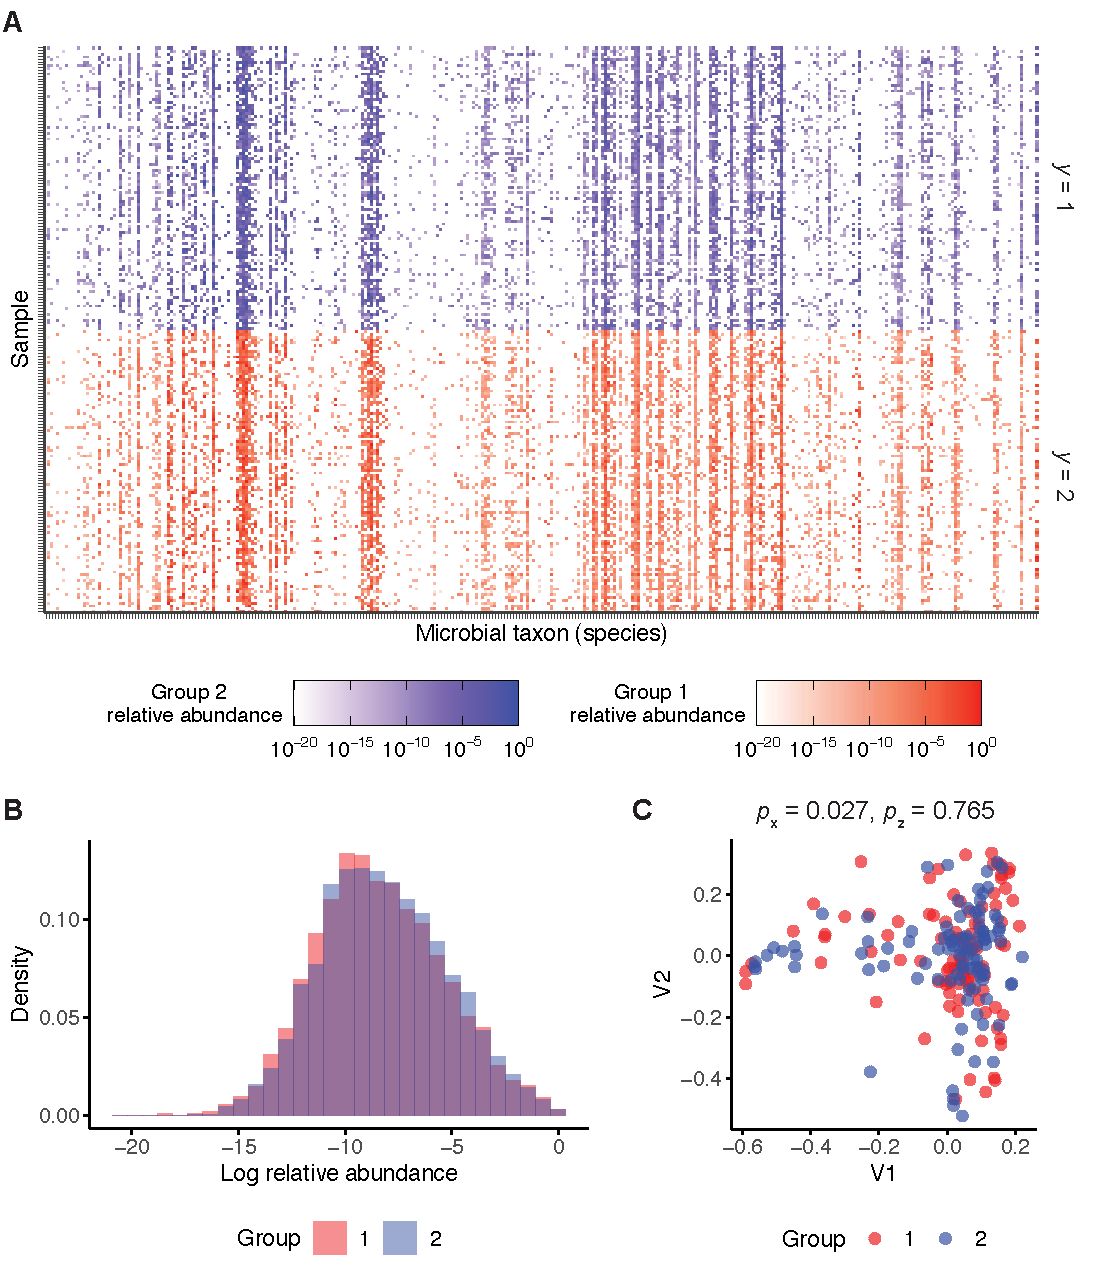
\includegraphics[width=6.5in]{submissions/plos/figures/Fig_S1_rev.pdf}
    \caption[Visualization of a semisynthetic dataset using SparseDOSSA.]{\DIFaddFL{Visualization }\DIFaddendFL of a \DIFdelbeginFL \DIFdelFL{simulated, binary }\DIFdelendFL \DIFaddbeginFL \DIFaddFL{semisynthetic }\DIFaddendFL dataset \DIFdelbeginFL \DIFdelFL{used in this study}\DIFdelendFL \DIFaddbeginFL \DIFaddFL{using SparseDOSSA}\DIFaddendFL . \DIFdelbeginFL \DIFdelFL{Axes }\DIFdelendFL \DIFaddbeginFL \DIFaddFL{(A) Heatmap }\DIFaddendFL of \DIFdelbeginFL \DIFdelFL{each plot correspond to orthonormal vectors that were obtained through eigendecomposition }\DIFdelendFL \DIFaddbeginFL \DIFaddFL{its log-scaled relative abundance by its microbial taxa and sample number. (B) Density histogram }\DIFaddendFL of the \DIFdelbeginFL \DIFdelFL{design matrix $\mathbf{X}$. Alignment on the axis v1 indicates that the samples have been normalized }\DIFdelendFL \DIFaddbeginFL \DIFaddFL{data and }\DIFaddendFL (\DIFdelbeginFL \DIFdelFL{Eq 9, main text}\DIFdelendFL \DIFaddbeginFL \DIFaddFL{C}\DIFaddendFL ) \DIFdelbeginFL \DIFdelFL{. Denoted }\DIFdelendFL \DIFaddbeginFL \DIFaddFL{principal coordinates analysis (PCoA) and PERMANOVA $p$-values based on PCoA results }\DIFaddendFL with \DIFdelbeginFL \DIFdelFL{different colors }\DIFdelendFL \DIFaddbeginFL \DIFaddFL{Euclidean distance ($p_\mathbf{z}$) }\DIFaddendFL and \DIFdelbeginFL \DIFdelFL{shapes are two groups that follow truncated normal distributions }\DIFdelendFL \DIFaddbeginFL \DIFaddFL{original structure }\DIFaddendFL with \DIFdelbeginFL \DIFdelFL{different means but the same covariance }\DIFdelendFL \DIFaddbeginFL \DIFaddFL{Bray-Curtis dissimilarity }\DIFaddendFL (\DIFdelbeginFL \DIFdelFL{Eq 8,main text.}\DIFdelendFL \DIFaddbeginFL \DIFaddFL{$p_\mathbf{x}$}\DIFaddendFL )\DIFaddbeginFL \DIFaddFL{. $N=200$ samples were generated as described.}\DIFaddendFL }
    \DIFdelbeginFL %DIFDELCMD < \label{fig:sim_data_2d}
%DIFDELCMD < %%%
\DIFdelendFL \DIFaddbeginFL \label{fig:sim_data_vis}
\DIFaddendFL \end{figure}
\clearpage

\DIFaddbegin \begin{figure}[h!]
    \centering
    \includegraphics[width=6.5in]{submissions/plos/figures/Fig_S2_rev.pdf}
    \caption[PERMANOVA $p$-values from $F$-informed MDS representations using semisynthetic data.]{\DIFaddFL{PERMANOVA $p$-values from $F$-informed MDS representations using semisynthetic data. $p$-values were plotted against the number of $F$-MDS training epochs for every hyperparameter $\lambda$. Triplicate datasets with size $N=50,100,200,500$ were evaluated. Once $p_\mathbf{z}$ reached to 1 during iteration, the majorization operation was discontinued (e.g., replicate 3 with $N=50$, $\lambda = 0.04$).}}
    \label{fig:sim_fmds_track}
\end{figure}
\clearpage

\DIFaddend \begin{figure}
    \centering
    \DIFdelbeginFL %DIFDELCMD < 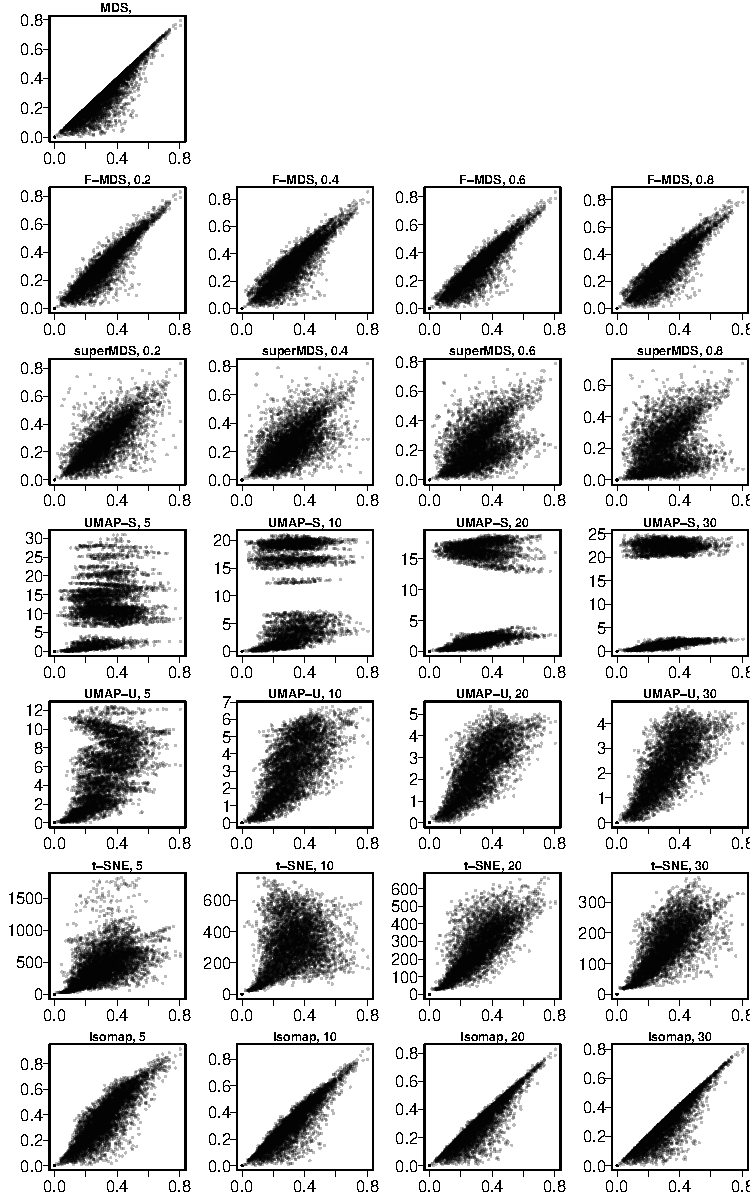
\includegraphics[width=5in]{submissions/plos/figures/Fig_S2.pdf}
%DIFDELCMD <     \caption[Shepard plot from 4D simulated dataset with seven ordination methods.]{%%%
\DIFdelFL{Shepard plot of simulated dataset (first replicate) }\DIFdelendFL \DIFaddbeginFL \includegraphics[width=6.5in]{submissions/plos/figures/Fig_S3_rev.pdf}
    \caption[Pairwise distance analyses from $F$-informed MDS and supervised MDS.]{\DIFaddFL{Pairwise distance analyses from $F$-informed MDS and supervised MDS }\DIFaddendFL using \DIFdelbeginFL \DIFdelFL{seven dimension reduction methods}\DIFdelendFL \DIFaddbeginFL \DIFaddFL{semisynthetic data}\DIFaddendFL . The plots are titled with the \DIFdelbeginFL \DIFdelFL{respective method }\DIFdelendFL \DIFaddbeginFL \DIFaddFL{dataset size $N$ }\DIFaddendFL and \DIFaddbeginFL \DIFaddFL{compared across different methods with }\DIFaddendFL hyperparameter values as follows: $\lambda$, $F$-MDS; $\alpha$, superMDS\DIFdelbeginFL \DIFdelFL{; Nearest neighbors number, supervised }\DIFdelendFL \DIFaddbeginFL \DIFaddFL{. After calculating pairwise distances with Bray-Curtis dissimilarity }\DIFaddendFL (\DIFdelbeginFL \DIFdelFL{-S}\DIFdelendFL \DIFaddbeginFL \DIFaddFL{original}\DIFaddendFL ) \DIFdelbeginFL \DIFdelFL{or unsupervised }\DIFdelendFL \DIFaddbeginFL \DIFaddFL{and Euclidean }\DIFaddendFL (\DIFdelbeginFL \DIFdelFL{-U}\DIFdelendFL \DIFaddbeginFL \DIFaddFL{2D representation}\DIFaddendFL )\DIFdelbeginFL \DIFdelFL{UMAP; Perplexity}\DIFdelendFL , \DIFdelbeginFL \DIFdelFL{t-SNE; Shortest dissimilarities number, Isomap. X- }\DIFdelendFL \DIFaddbeginFL \DIFaddFL{(B) their Pearson correlation coefficient }\DIFaddendFL and \DIFdelbeginFL \DIFdelFL{Y-axis denote the pairwise distance in the original and embedding dimensions, respectively}\DIFdelendFL \DIFaddbeginFL \DIFaddFL{(C) normalized stress (Stress-1) were obtained}\DIFaddendFL . \DIFaddbeginFL \DIFaddFL{Error bars are standard deviation of triplicates.}\DIFaddendFL }
    \DIFdelbeginFL %DIFDELCMD < \label{fig:shepard_sim_all}
%DIFDELCMD < %%%
\DIFdelendFL \DIFaddbeginFL \label{fig:sim_fmds_smds}
\DIFaddendFL \end{figure}
\clearpage

\begin{figure}
    \centering
    \DIFdelbeginFL %DIFDELCMD < \includegraphics[width=5in]{submissions/plos/figures/Fig_S3.pdf}
%DIFDELCMD <     \caption[\textit{F}-correlation plot from simulated dataset.]{%%%
\textit{\DIFdelFL{F}}%DIFAUXCMD
\DIFdelFL{-correlation plot with simulated data. Pseudo }\DIFdelendFL \DIFaddbeginFL \includegraphics[width=6.5in]{submissions/plos/figures/Fig_S4_rev_gridsearch.pdf}
    \caption[Hyperparameter selection using grid search.]{\DIFaddFL{Hyperparameter selection for }\DIFaddendFL $F$\DIFdelbeginFL \DIFdelFL{-ratios were calculated in }\DIFdelendFL \DIFaddbeginFL \DIFaddFL{-informed MDS using grid search. An objective function $f_{\rm obj}(\lambda)$ was defined to simultaneously reflect }\DIFaddendFL the \DIFaddbeginFL \DIFaddFL{number of training epochs and the preservation of the }\DIFaddendFL original \DIFdelbeginFL \DIFdelFL{dimension }\DIFdelendFL \DIFaddbeginFL \DIFaddFL{structure }\DIFaddendFL (\DIFdelbeginFL \DIFdelFL{x-axis}\DIFdelendFL \DIFaddbeginFL \DIFaddFL{see Equation \ref{eq:def_grid_search}}\DIFaddendFL )\DIFdelbeginFL \DIFdelFL{and in each dimension reduction method }\DIFdelendFL \DIFaddbeginFL \DIFaddFL{. }\DIFaddendFL (\DIFdelbeginFL \DIFdelFL{y-axis}\DIFdelendFL \DIFaddbeginFL \DIFaddFL{A}\DIFaddendFL ) \DIFdelbeginFL \DIFdelFL{using first replicate of the simulated }\DIFdelendFL \DIFaddbeginFL \DIFaddFL{For each semisynthetic }\DIFaddendFL dataset \DIFdelbeginFL \DIFdelFL{. Pseudo $F$'s were calculated by randomly permuting labels by 500 times. Highlighted with red denotes }\DIFdelendFL \DIFaddbeginFL \DIFaddFL{size $N$, $f_{\rm obj}(\lambda)$ is plotted against }\DIFaddendFL the \DIFdelbeginFL \DIFdelFL{location }\DIFdelendFL \DIFaddbeginFL \DIFaddFL{hyperparameter $\lambda$. The minimum value }\DIFaddendFL of \DIFdelbeginFL \DIFdelFL{$F$'s from unpermuted labels}\DIFdelendFL \DIFaddbeginFL \DIFaddFL{$f_{\rm obj}(\lambda)$ is highlighted in red}\DIFaddendFL . \DIFdelbeginFL \DIFdelFL{Each plot }\DIFdelendFL \DIFaddbeginFL \DIFaddFL{(B) The optimal hyperparameter $\lambda_{\rm min}$ }\DIFaddendFL is \DIFdelbeginFL \DIFdelFL{titled }\DIFdelendFL \DIFaddbeginFL \DIFaddFL{plotted against dataset size $N$, }\DIFaddendFL with \DIFdelbeginFL \DIFdelFL{the method and hyperparameter used}\DIFdelendFL \DIFaddbeginFL \DIFaddFL{each dataset represented by a symbol}\DIFaddendFL .}
    \DIFdelbeginFL %DIFDELCMD < \label{fig:f_corr_sim_all}
%DIFDELCMD < %%%
\DIFdelendFL \DIFaddbeginFL \label{fig:fmds_gridsearch}
\DIFaddendFL \end{figure}
\clearpage

\begin{figure}
    \centering
    \DIFdelbeginFL %DIFDELCMD < \includegraphics[width=5in]{submissions/plos/figures/Fig_S4.pdf}
%DIFDELCMD <     %%%
%DIFDELCMD < \caption[Shepard plot from algal microbiome dataset with eight ordination methods.]{%
{%DIFAUXCMD
\DIFdelFL{Shepard plot of algal-associated bacterial community data using eight dimension reduction methods. The plots are titled with the respective method and hyperparameter values as follows: $\lambda$, $F$-MDS; $\alpha$, superMDS; Nearest neighbors number, supervised (-S) or unsupervised (-U) UMAP; Perplexity, t-SNE; Shortest dissimilarities number, Isomap; none, neural network (NN). X- and Y-axis denote distances in the original and embedding dimensions, respectively.}}
    %DIFAUXCMD
%DIFDELCMD < \label{fig:shepard_alga_all}
%DIFDELCMD < %%%
\DIFdelendFL \DIFaddbeginFL \includegraphics[width=5.05in]{submissions/plos/figures/Fig_S5_rev.pdf}
    \caption[Comparison of quality metrics of benchmark ordination methods.]{\DIFaddFL{Comparison of quality metrics of ordination methods evaluated on semisynthetic datasets. Trustworthiness and continuity to evaluate (A) Local structural preservation is assessed using trustworthiness and continuity. (B) Global structural preservation is similarly evaluated with trustworthiness and continuity. (C) Global distortion is quantified by Stress-1 and Pearson correlation of Shepard diagrams. (D) Preservation of statistical inference is measured by the $F$-rank-ratio and $F$-correlation using randomly permuted label sets. The following hyperparameters were used for each method: $\lambda$ for $F$-MDS, number of neighbors $n$ for UMAP (both supervised (-S) and unsupervised (-U)), perplexity (perp) for t-SNE, and the number of shortest dissimilarities $n$ for Isomap. Error bars represent the standard deviation across triplicate measurements.}}
    \label{fig:sim_eval_all}
\DIFaddendFL \end{figure}
\clearpage

\begin{figure}
    \centering
    \DIFdelbeginFL %DIFDELCMD < \includegraphics[width=5in]{submissions/plos/figures/Fig_S5.pdf}
%DIFDELCMD <     %%%
%DIFDELCMD < \caption[\textit{F}-correlation plot from algal microbiome dataset.]{%
{%DIFAUXCMD
\textit{\DIFdelFL{F}}%DIFAUXCMD
\DIFdelFL{-correlation plot from algal microbiome dataset. Pseudo $F$-ratios comparing the original dimension (x-axis) and from eight dimension reduction methods (y-axis) with algal microbiome data. Pseudo $F$'s were calculated by randomly permuting labels by 500 times. Highlighted with red denotes the location of $F$'s from unpermuted labels. Each plot is titled with the method and hyperparameter used.}}
    %DIFAUXCMD
%DIFDELCMD < \label{fig:f_corr_alga_all}
%DIFDELCMD < %%%
\DIFdelendFL \DIFaddbeginFL \includegraphics[width=5in]{submissions/plos/figures/Fig_S6_rev.pdf}
    \caption[Shepard plot from algal microbiome dataset with eight ordination methods.]{\DIFaddFL{Shepard plot of algal-associated bacterial community data using eight dimension reduction methods. The plots are titled with the respective method and hyperparameter values as follows: $\lambda$, $F$-MDS; $\alpha$, superMDS; Nearest neighbors number, supervised (-S) or unsupervised (-U) UMAP; Perplexity, t-SNE; Shortest dissimilarities number, Isomap; none, neural network (NN). X- and Y-axis denote distances in the original and embedding dimensions, respectively.}}
    \label{fig:shepard_alga_all}
\DIFaddendFL \end{figure}
\clearpage

\begin{figure}
    \centering
    \DIFdelbeginFL %DIFDELCMD < \includegraphics[width=6.5in]{submissions/plos/figures/Fig_S6.pdf}
%DIFDELCMD <     \caption[Pairs plot of simulated, trinary data.]{%%%
\DIFdelFL{Pairs plot of trinary, four-dimensional simulated data. Each row and column corresponds to respective axis for the projection. Denoted with different colors or shapes are the trinary groups that follow normal distributions with different means but the same covariance (Eq 10, main text.) }%DIFDELCMD < \MBLOCKRIGHTBRACE
%DIFDELCMD <     \label{fig:sim_data_4d}
%DIFDELCMD < %%%
\DIFdelendFL \DIFaddbeginFL \includegraphics[width=5in]{submissions/plos/figures/Fig_S7_rev.pdf}
    \caption[\textit{F}-correlation plot from algal microbiome dataset.]{\textit{\DIFaddFL{F}}\DIFaddFL{-correlation plot from algal microbiome dataset. Pseudo $F$-ratios comparing the original dimension (x-axis) and from eight dimension reduction methods (y-axis) with algal microbiome data. Pseudo $F$'s were calculated by randomly permuting labels by 500 times. Highlighted with red denotes the location of $F$'s from unpermuted labels. Each plot is titled with the method and hyperparameter used.}}
    \label{fig:f_corr_alga_all}
\DIFaddendFL \end{figure}
\clearpage

\begin{figure}
    \centering
    \DIFdelbeginFL %DIFDELCMD < \includegraphics[width=6.5in]{submissions/plos/figures/Fig_S7.pdf}
%DIFDELCMD <     %%%
\DIFdelendFL \DIFaddbeginFL \includegraphics[width=6.5in]{submissions/plos/figures/Fig_S8_rev.pdf}
    \DIFaddendFL \caption[Cluster centroid and variances of $F$-MDS representations.]{Cluster \DIFdelbeginFL \DIFdelFL{centroid }\DIFdelendFL \DIFaddbeginFL \DIFaddFL{centroids }\DIFaddendFL and variances of $F$-MDS representations \DIFaddbeginFL \DIFaddFL{are shown }\DIFaddendFL for \DIFdelbeginFL \DIFdelFL{simulated dataset }\DIFdelendFL \DIFaddbeginFL \DIFaddFL{semisynthetic datasets of size $N=50$ }\DIFaddendFL (\DIFdelbeginFL \DIFdelFL{A-C}\DIFdelendFL \DIFaddbeginFL \DIFaddFL{A–C}\DIFaddendFL )\DIFaddbeginFL \DIFaddFL{, $N=100$ (D–F), $N=200$ (G–I), $N=500$ (J–L) }\DIFaddendFL and \DIFaddbeginFL \DIFaddFL{for the }\DIFaddendFL algal microbiome (\DIFdelbeginFL \DIFdelFL{D-F}\DIFdelendFL \DIFaddbeginFL \DIFaddFL{M–O}\DIFaddendFL ). \DIFdelbeginFL \DIFdelFL{A,D: Distance }\DIFdelendFL \DIFaddbeginFL \DIFaddFL{The first column in each row displays the distance }\DIFaddendFL between group centroids. \DIFdelbeginFL \DIFdelFL{B,E: Variance }\DIFdelendFL \DIFaddbeginFL \DIFaddFL{The second and third columns show the variance }\DIFaddendFL of each group\DIFdelbeginFL \DIFdelFL{measured in its long-axis. C}\DIFdelendFL , \DIFdelbeginFL \DIFdelFL{F: Variance of each group }\DIFdelendFL measured \DIFdelbeginFL \DIFdelFL{in its short-axis}\DIFdelendFL \DIFaddbeginFL \DIFaddFL{along the long and short principal axes, respectively}\DIFaddendFL . For \DIFdelbeginFL \DIFdelFL{simulated dataset error bars denote standard deviation of triplicates. For }\DIFdelendFL \DIFaddbeginFL \DIFaddFL{the }\DIFaddendFL variance \DIFdelbeginFL \DIFdelFL{calculations}\DIFdelendFL \DIFaddbeginFL \DIFaddFL{panels}\DIFaddendFL , blue and red colors denote \DIFdelbeginFL \DIFdelFL{group }\DIFdelendFL \DIFaddbeginFL \DIFaddFL{groups }\DIFaddendFL 1 and \DIFdelbeginFL \DIFdelFL{2, respectively}\DIFdelendFL \DIFaddbeginFL \DIFaddFL{2. Error bars represent the standard deviation across triplicate measurements}\DIFaddendFL .}
    \label{fig:fmds_rep_analysis}
\end{figure}
\clearpage

%DIF <  \begin{figure}
%DIF <      \centering
%DIF <      \includegraphics[width=6.5in]{submissions/nips/figures/site-config-all.pdf}
%DIF <      \caption[Visualization of bacterial community using FMDS.]{Visualization of bacterial community using proposed FMDS. Microbial community samples are collected from Site 1 (top row) and Site 2 (bottom row).}
%DIF <      \label{fig:site_config_all}
%DIF <  \end{figure}
%DIF <  \clearpage
\DIFdelbegin %DIFDELCMD < 

%DIFDELCMD < %%%
%DIF <  \begin{figure}
%DIF <      \centering
%DIF <      \includegraphics[width=6.5in]{submissions/nips/figures/shepard_site.png}
%DIF <      \caption[Shepard plot of community dataset.]{Shepard plot in microbial community data collected from site 1 (first row) and site 2 (second row) for a range of hyperparameters.}
%DIF <      \label{fig:shepard_site}
%DIF <  \end{figure}
%DIF <  \clearpage
%DIFDELCMD < 

%DIFDELCMD < %%%
%DIF <  \begin{figure}
%DIF <      \centering
%DIF <      \includegraphics[width=6.5in]{submissions/ISMB/figures/cirrhosis.pdf}
%DIF <      \caption[Visualization of cirrhosis patients and healthy human gut microbiome.]{Visualization of cirrhosis patients and healthy human gut microbiome. The following hyperparameters were used: $\lambda=0.3$ (FMDS), neighbors $=10$ (UMAP-S), neighbors $=30$ (UMAP-U), perplexity$=7$ (t-SNE), $K=10$ (Isomap).}
%DIF <      \label{fig:cirr}
%DIF <  \end{figure}
%DIF <  \clearpage
\DIFdelend \DIFaddbegin \begin{figure}
    \centering
    \includegraphics[width=6.5in]{submissions/plos/figures/Fig_S9_rev.pdf}
    \caption[Visualization of a semisynthetic ternary dataset.]{\DIFaddFL{Visualization of a semisynthetic ternary dataset. (A) Heatmap of its log-scaled relative abundance by its microbial taxa and sample number. (B) Density histogram of the data and (C) principal coordinates analysis (PCoA) and PERMANOVA $p$-values based on PCoA results with Euclidean distance ($p_\mathbf{z}$) and original structure with Bray-Curtis dissimilarity ($p_\mathbf{x}$). $N=75$ semisynthetic data were generated.}}
    \label{fig:sim_ternary_vis}
\end{figure}
\clearpage
\DIFaddend 


\begin{singlespace}
\bibliographystyle{acm}
\documentclass[11pt]{article}
%DIF LATEXDIFF DIFFERENCE FILE


%%%%%%%%%%%%%%%%%%%%%%%%%%%%%%%%%%%%%%%%%%%%%%%%%%%%%%%%%
%%%%%%%%%%%%%%%%%%%%%%%%% Setup %%%%%%%%%%%%%%%%%%%%%%%%%
\usepackage[margin=1in]{geometry}
\usepackage{fmtcount} % 1st, 2nd...
\usepackage[english]{babel}
\usepackage{soul} % spacing
\usepackage{enumerate} % change enum label
\usepackage{framed} % frame pagebreak
\usepackage{authblk}
\usepackage{setspace}
\usepackage{tocloft}

%%%%% Math, Code 
\usepackage{amsmath}
\usepackage{amsfonts}
\usepackage{amssymb}
\usepackage{amsthm}
\usepackage{amscd}
\usepackage{array}
\usepackage{mathtools} 
\usepackage{verbatim}
\usepackage{fancyvrb} % verbatim
\usepackage{algpseudocode}
\usepackage{algorithm}

%%%%% Graphic, Figure, Table
\usepackage{graphicx}
\usepackage{epstopdf}
\usepackage{xcolor}
\usepackage[labelsep=none]{caption}
\usepackage{subcaption}
\usepackage{multirow} % table
\usepackage{longtable} % table to next page
\usepackage{rotating}
\usepackage{wrapfig} % wrap fig, tbl with text

%%%%% Bib, Cite
\usepackage{url}
\usepackage{cite}
\usepackage{fancyref}
\usepackage{hyperref}
\hypersetup{linktocpage}

%%%%%% Setup
% \captionsetup{compatibility=false} %subfig
% \DeclareCaptionLabelFormat{Sformat}{S#2 #1}
% \captionsetup[figure]{labelformat=Sformat}
% \captionsetup[table]{labelformat=Sformat}
\hypersetup{colorlinks=false}
\setlength{\parskip}{0.5em}

\newtheorem{thm}{Theorem}[section]
\newtheorem{cor}[thm]{Corollary}
\newtheorem{lem}[thm]{Lemma}
\newtheorem{prop}[thm]{Proposition}
\newtheorem{dfn}{Definition}
\newtheorem{ex}{Example}
\newtheorem{cmt}{Cmt}[section]
\newtheorem{rmk}{Remark}[section]
\newcommand{\rb}[1]{\raisebox{-.5em}[0pt]{#1}}
\newcommand{\1}{{\rm 1}\kern-0.24em{\rm I}}
\newcommand{\cN}{\mathcal{N}}
\newcommand{\cO}{\mathcal{O}}
\renewcommand{\mid}{\, | \ , }
\makeatletter
\renewcommand\theequation{S\@arabic\c@equation}
\makeatother

\renewcommand\Affilfont{\normalsize}
% \renewcommand{\baselinestretch}{1.3}

\DeclareMathOperator*{\argmin}{arg\,min}
\DeclareMathOperator*{\argmax}{arg\,max}
\DeclareMathOperator*{\bbr}{\mathbb{R}}
%%%%%%%%%%%%%%%%%%%%%%%%%%%%%%%%%%%%%%%%%%%%%%%%%%%%%%%
%%%%%%%%%%%%%%%%%%%%%%%%%%%%%%%%%%%%%%%%%%%%%%%%%%%%%%%

\title{Supporting Information of ``Multidimensional scaling informed by $F$-statistic: Visualizing grouped microbiome data with inference''}
\author[1\dag]{Hyungseok Kim}
\author[2\dag]{Soobin Kim}
\author[3]{Jeffrey A. Kimbrel}
\author[3]{Megan M. Morris}
\author[3]{Xavier Mayali}
\author[1$*$]{Cullen R. Buie}
\affil[1]{Massachusetts Institute of Technology, Cambridge, MA, USA}
\affil[2]{University of California, Davis, Davis, CA, USA}
\affil[3]{Lawrence Livermore National Laboratory, Livermore, CA, USA}
\affil[$\dagger$] {These authors contributed equally to this work.}
\affil[$^*$]{Correspondence: crb@mit.edu.}
% \author{}
\date{}
%DIF PREAMBLE EXTENSION ADDED BY LATEXDIFF
%DIF UNDERLINE PREAMBLE %DIF PREAMBLE
\RequirePackage[normalem]{ulem} %DIF PREAMBLE
\RequirePackage{color}\definecolor{RED}{rgb}{1,0,0}\definecolor{BLUE}{rgb}{0,0,1} %DIF PREAMBLE
\providecommand{\DIFaddtex}[1]{{\protect\color{blue}\uwave{#1}}} %DIF PREAMBLE
\providecommand{\DIFdeltex}[1]{{\protect\color{red}\sout{#1}}}                      %DIF PREAMBLE
%DIF SAFE PREAMBLE %DIF PREAMBLE
\providecommand{\DIFaddbegin}{} %DIF PREAMBLE
\providecommand{\DIFaddend}{} %DIF PREAMBLE
\providecommand{\DIFdelbegin}{} %DIF PREAMBLE
\providecommand{\DIFdelend}{} %DIF PREAMBLE
\providecommand{\DIFmodbegin}{} %DIF PREAMBLE
\providecommand{\DIFmodend}{} %DIF PREAMBLE
%DIF FLOATSAFE PREAMBLE %DIF PREAMBLE
\providecommand{\DIFaddFL}[1]{\DIFadd{#1}} %DIF PREAMBLE
\providecommand{\DIFdelFL}[1]{\DIFdel{#1}} %DIF PREAMBLE
\providecommand{\DIFaddbeginFL}{} %DIF PREAMBLE
\providecommand{\DIFaddendFL}{} %DIF PREAMBLE
\providecommand{\DIFdelbeginFL}{} %DIF PREAMBLE
\providecommand{\DIFdelendFL}{} %DIF PREAMBLE
%DIF HYPERREF PREAMBLE %DIF PREAMBLE
\providecommand{\DIFadd}[1]{\texorpdfstring{\DIFaddtex{#1}}{#1}} %DIF PREAMBLE
\providecommand{\DIFdel}[1]{\texorpdfstring{\DIFdeltex{#1}}{}} %DIF PREAMBLE
\newcommand{\DIFscaledelfig}{0.5}
%DIF HIGHLIGHTGRAPHICS PREAMBLE %DIF PREAMBLE
\RequirePackage{settobox} %DIF PREAMBLE
\RequirePackage{letltxmacro} %DIF PREAMBLE
\newsavebox{\DIFdelgraphicsbox} %DIF PREAMBLE
\newlength{\DIFdelgraphicswidth} %DIF PREAMBLE
\newlength{\DIFdelgraphicsheight} %DIF PREAMBLE
% store original definition of \includegraphics %DIF PREAMBLE
\LetLtxMacro{\DIFOincludegraphics}{\includegraphics} %DIF PREAMBLE
\newcommand{\DIFaddincludegraphics}[2][]{{\color{blue}\fbox{\DIFOincludegraphics[#1]{#2}}}} %DIF PREAMBLE
\newcommand{\DIFdelincludegraphics}[2][]{% %DIF PREAMBLE
\sbox{\DIFdelgraphicsbox}{\DIFOincludegraphics[#1]{#2}}% %DIF PREAMBLE
\settoboxwidth{\DIFdelgraphicswidth}{\DIFdelgraphicsbox} %DIF PREAMBLE
\settoboxtotalheight{\DIFdelgraphicsheight}{\DIFdelgraphicsbox} %DIF PREAMBLE
\scalebox{\DIFscaledelfig}{% %DIF PREAMBLE
\parbox[b]{\DIFdelgraphicswidth}{\usebox{\DIFdelgraphicsbox}\\[-\baselineskip] \rule{\DIFdelgraphicswidth}{0em}}\llap{\resizebox{\DIFdelgraphicswidth}{\DIFdelgraphicsheight}{% %DIF PREAMBLE
\setlength{\unitlength}{\DIFdelgraphicswidth}% %DIF PREAMBLE
\begin{picture}(1,1)% %DIF PREAMBLE
\thicklines\linethickness{2pt} %DIF PREAMBLE
{\color[rgb]{1,0,0}\put(0,0){\framebox(1,1){}}}% %DIF PREAMBLE
{\color[rgb]{1,0,0}\put(0,0){\line( 1,1){1}}}% %DIF PREAMBLE
{\color[rgb]{1,0,0}\put(0,1){\line(1,-1){1}}}% %DIF PREAMBLE
\end{picture}% %DIF PREAMBLE
}\hspace*{3pt}}} %DIF PREAMBLE
} %DIF PREAMBLE
\LetLtxMacro{\DIFOaddbegin}{\DIFaddbegin} %DIF PREAMBLE
\LetLtxMacro{\DIFOaddend}{\DIFaddend} %DIF PREAMBLE
\LetLtxMacro{\DIFOdelbegin}{\DIFdelbegin} %DIF PREAMBLE
\LetLtxMacro{\DIFOdelend}{\DIFdelend} %DIF PREAMBLE
\DeclareRobustCommand{\DIFaddbegin}{\DIFOaddbegin \let\includegraphics\DIFaddincludegraphics} %DIF PREAMBLE
\DeclareRobustCommand{\DIFaddend}{\DIFOaddend \let\includegraphics\DIFOincludegraphics} %DIF PREAMBLE
\DeclareRobustCommand{\DIFdelbegin}{\DIFOdelbegin \let\includegraphics\DIFdelincludegraphics} %DIF PREAMBLE
\DeclareRobustCommand{\DIFdelend}{\DIFOaddend \let\includegraphics\DIFOincludegraphics} %DIF PREAMBLE
\LetLtxMacro{\DIFOaddbeginFL}{\DIFaddbeginFL} %DIF PREAMBLE
\LetLtxMacro{\DIFOaddendFL}{\DIFaddendFL} %DIF PREAMBLE
\LetLtxMacro{\DIFOdelbeginFL}{\DIFdelbeginFL} %DIF PREAMBLE
\LetLtxMacro{\DIFOdelendFL}{\DIFdelendFL} %DIF PREAMBLE
\DeclareRobustCommand{\DIFaddbeginFL}{\DIFOaddbeginFL \let\includegraphics\DIFaddincludegraphics} %DIF PREAMBLE
\DeclareRobustCommand{\DIFaddendFL}{\DIFOaddendFL \let\includegraphics\DIFOincludegraphics} %DIF PREAMBLE
\DeclareRobustCommand{\DIFdelbeginFL}{\DIFOdelbeginFL \let\includegraphics\DIFdelincludegraphics} %DIF PREAMBLE
\DeclareRobustCommand{\DIFdelendFL}{\DIFOaddendFL \let\includegraphics\DIFOincludegraphics} %DIF PREAMBLE
%DIF END PREAMBLE EXTENSION ADDED BY LATEXDIFF

\begin{document}

\renewcommand*\contentsname{\normalsize List of Supplementary Notes}
\makeatletter
\renewcommand{\tableofcontents}{\@starttoc{toc}}
\renewcommand*\l@section{\@dottedtocline{1}{0em}{6.3em}}
\let\l@table\l@content
\makeatother

\makeatletter
\renewcommand{\listoffigures}{\@starttoc{lof}}
\renewcommand*\l@figure{\@dottedtocline{1}{0em}{3.5em}}
\let\l@table\l@figure
\makeatother

\makeatletter
\renewcommand{\listoftables}{\@starttoc{lot}}
\renewcommand*\l@table{\@dottedtocline{1}{0em}{4.5em}}
\let\l@table\l@table
\makeatother

\renewcommand\thesection{S\arabic{section} Appendix.}
\makeatletter
\renewcommand*{\@seccntformat}[1]{\csname the#1\endcsname\hspace{0.5em}}
\makeatother

\renewcommand{\figurename}{\!\!}
\let\standardthefigure\thefigure
\renewcommand\thefigure{S\standardthefigure\ Fig.\ }
\addtolength{\cftfignumwidth}{15pt}

\renewcommand{\tablename}{\!\!}
\let\standardthetable\thetable
\renewcommand\thetable{S\standardthetable\ Table.\ }

% \renewcommand{\algorithmname}{\!\!}
\let\standardthealgorithm\thealgorithm
\renewcommand\thealgorithm{S\standardthealgorithm}

\maketitle
% \def\thefootnote{\arabic{footnote}}

{\noindent\normalsize\bf List of Supplementary Information}
\tableofcontents
\listoffigures
\listoftables
\clearpage


\section{\DIFdelbegin \DIFdel{Mapping }\DIFdelend \DIFaddbegin \DIFadd{Objective }\DIFaddend function for \DIFaddbegin \DIFadd{computing }\DIFaddend $F$-MDS\DIFdelbegin \DIFdel{.}\DIFdelend } \label{sec:app1}

\DIFdelbegin \DIFdel{In this section, we explain a procedure of deriving a }\DIFdelend \DIFaddbegin \DIFadd{First, we derive a }\DIFaddend mapping function $f_\mathbf{z}(F_\mathbf{x})$ \DIFdelbegin \DIFdel{that is used to minimize }\DIFdelend \DIFaddbegin \DIFadd{for minimizing }\DIFaddend an objective function \DIFdelbegin \DIFdel{for }\DIFdelend \DIFaddbegin \DIFadd{and }\DIFaddend computing $F$-informed MDS.
The \DIFdelbegin \DIFdel{confirmatory term of the objective function (Eq 5 of the main text) is specifically designed }\DIFdelend \DIFaddbegin \DIFadd{mapping function guides }\DIFaddend to minimize a difference in $p$-values testing \DIFdelbegin \DIFdel{for group difference by representations }\DIFdelend \DIFaddbegin \DIFadd{group differences }\DIFaddend under the original $S$- and \DIFdelbegin \DIFdel{two-dimensions}\DIFdelend \DIFaddbegin \DIFadd{two-dimensional embedding through the confirmatory term of the objective (see Eq 5 of the main text)}\DIFaddend .
These \textit{p}-values are obtained from an empirical distribution of the pseudo-$F$s by permuted labels \cite{anderson01} \DIFdelbegin \DIFdel{. 
In other words, by denoting a label set as $[y_i]$ ($i=1,\cdots N$) and its permuted set as $[y_i^\pi]$ with operator $\pi$, we express each }\DIFdelend \DIFaddbegin \DIFadd{(Eq 4, main text). 
For a given label set $[y_i]_{i=1}^{N}$ and its group number $G$, a permuted label set $[y_i^\Pi]_{i=1}^{N}$ and }\DIFaddend $F$\DIFdelbegin \DIFdel{-statistic as
}\DIFdelend \DIFaddbegin \DIFadd{-statistics are expressed as
}\DIFaddend \begin{equation}
\DIFdelbegin %DIFDELCMD < \begin{aligned}
%DIFDELCMD < F^\pi_\mathbf{x} &= 
%DIFDELCMD < \left(\frac{\sum_{i,j}d_{ij}^2}{2\sum_{i,j}d_{ij}^2\,\1\{y_i^\pi = y_j^\pi\}} -1 \right) \cdot (N-2), \\
%DIFDELCMD < F^\pi_\mathbf{z} &= 
%DIFDELCMD < \left(\frac{\sum_{i,j}\|\mathbf{z}_i - \mathbf{z}_j\|_2^2}{2\sum_{i,j}\|\mathbf{z}_i - \mathbf{z}_j\|_2^2\,\1\{y_i^\pi = y_j^\pi\}} -1 \right) \cdot (N-2).
%DIFDELCMD < \label{eq:map1}
%DIFDELCMD < \end{aligned}%%%
\DIFdelend \DIFaddbegin \begin{aligned}
F^\Pi_\mathbf{x} &= 
\left(\frac{\sum_{i,j}d_{ij}^2}{G \sum_{i,j}d_{ij}^2\,\1\{y_i^\Pi = y_j^\Pi\}} -1 \right) \cdot \frac{N-G}{G-1}, \\
F^\Pi_\mathbf{z} &= 
\left(\frac{\sum_{i,j}\|\mathbf{z}_i - \mathbf{z}_j\|_2^2}{G\sum_{i,j}\|\mathbf{z}_i - \mathbf{z}_j\|_2^2\,\1\{y_i^\Pi = y_j^\Pi\}} -1 \right) \cdot \frac{N-G}{G-1}.
\label{eq:map1}
\end{aligned}\DIFaddend 
\end{equation}
% \end{align} 

It should be noted that the pseudo $F$-ratios can range differently based on how the samples are projected onto 2D. To scale between these two ratios and minimize the difference in $p$-values, we consider a mapping $f_\mathbf{z}: F_\mathbf{x} \rightarrow F_\mathbf{z}$ from a pair of ratios \DIFdelbegin \DIFdel{$(F_\mathbf{x}^{\pi_1}, F_\mathbf{z}^{\pi_2})$ }\DIFdelend \DIFaddbegin \DIFadd{$(F_\mathbf{x}^{\Pi_1}, F_\mathbf{z}^{\Pi_2})$ }\DIFaddend where each element was ordered from two independent sets of repeated permutations. Figure below exemplifies how the $F$-ratios at each dimensionality scaled differently and depended on the choice of hyperparameter $\lambda$. In both settings, the $F$-ratio in $S$-dimension ranged \DIFdelbegin \DIFdel{between zero and six }\DIFdelend \DIFaddbegin \DIFadd{in }[\DIFadd{0,6}] \DIFaddend whereas in 2D representation the ratio ranged in [0,4]. The hyperparameter, however, impacted the detailed relationship between ordered $F_\mathbf{x}$ and ordered $F_\mathbf{x}$, when compared to each other. 

\begin{figure}[h]
    \centering
    \includegraphics[width=5.5in]{submissions/plos/figures/supp-mds_Fval.pdf}
    \caption*{Figure: Mapping pseudo-$F$'s between two dimensionalities. Each $F_\mathbf{x} \text{-} F_\mathbf{z}$ relationship was obtained by permuting labels over 1,000 times, and by setting a hyperparameter $\lambda$ that is used to perform the majorization.}
    \label{fig:mds-fval}
\end{figure}

Using the mapping function $f_\mathbf{z}$, we \DIFdelbegin \DIFdel{now }\DIFdelend derive an exact \DIFdelbegin \DIFdel{form of confirmatory term proposed }\DIFdelend \DIFaddbegin \DIFadd{expression for the confirmatory term introduced }\DIFaddend in the $F$-MDS objective function\DIFdelbegin \DIFdel{(Eq 5 of main text)}\DIFdelend . The proposed form $\left|F_\mathbf{z} - f_\mathbf{z}(F_\mathbf{x})\right|$ measures how \DIFaddbegin \DIFadd{accurately }\DIFaddend the 2D representation \DIFdelbegin \DIFdel{accurately reflected }\DIFdelend \DIFaddbegin \DIFadd{reflects }\DIFaddend the $S$-dimensional distance structure \DIFdelbegin \DIFdel{with respect to }\DIFdelend \DIFaddbegin \DIFadd{regarding }\DIFaddend the sample labels. \DIFdelbegin \DIFdel{Having the }\DIFdelend \DIFaddbegin \DIFadd{A }\DIFaddend difference close to zero indicates that no \DIFdelbegin \DIFdel{additional update with the representation is required (let us denote it as }\DIFdelend \DIFaddbegin \DIFadd{further updates to the representation are required (denoted }\DIFaddend $\mathbf{Z}^*$). \DIFdelbegin \DIFdel{Now by substituting }\DIFdelend \DIFaddbegin \DIFadd{Substituting }\DIFaddend the confirmatory term $\left|F_\mathbf{z} - f_\mathbf{z}(F_\mathbf{x})\right|$ with Equation \ref{eq:map1}, we define \DIFdelbegin \DIFdel{$\1\{y_i^\pi = y_j^\pi\}\coloneqq\epsilon_{ij}$ and write
}\DIFdelend \DIFaddbegin \DIFadd{$\epsilon_{ij}\coloneqq\1\{y_i^\Pi = y_j^\Pi\}$ and write
}\DIFaddend \begin{align}
\mathbf{Z}^* &= \argmin_\mathbf{Z}\,\left|F_\mathbf{z} - f_\mathbf{z}(F_\mathbf{x})\right| \\
& = \argmin_\mathbf{Z}\,\left|\DIFdelbegin \DIFdel{(N-2)}\DIFdelend \DIFaddbegin \DIFadd{\frac{N-G}{G-1}}\DIFaddend \cdot\left(\DIFdelbegin \DIFdel{\frac{\sum_{i,j}\|\mathbf{z}_i - \mathbf{z}_j\|_2^2}{2\sum_{i,j}\epsilon_{ij}\|\mathbf{z}_i - \mathbf{z}_j\|_2^2} }\DIFdelend \DIFaddbegin \DIFadd{\frac{\sum_{i,j}\|\mathbf{z}_i - \mathbf{z}_j\|_2^2}{G\sum_{i,j}\epsilon_{ij}\|\mathbf{z}_i - \mathbf{z}_j\|_2^2} }\DIFaddend -1 \right) - f_\mathbf{z}(F_\mathbf{x})\right| \\
&= \argmin_\mathbf{Z}\,\left|\DIFdelbegin \DIFdel{\frac{\sum_{i,j}\|\mathbf{z}_i - \mathbf{z}_j\|_2^2}{2\sum_{i,j}\epsilon_{ij}\|\mathbf{z}_i - \mathbf{z}_j\|_2^2} }\DIFdelend \DIFaddbegin \DIFadd{\frac{\sum_{i,j}\|\mathbf{z}_i - \mathbf{z}_j\|_2^2}{G\sum_{i,j}\epsilon_{ij}\|\mathbf{z}_i - \mathbf{z}_j\|_2^2} }\DIFaddend -1 - \DIFdelbegin \DIFdel{\frac{f_\mathbf{z}(F_\mathbf{x})}{N-2} }\DIFdelend \DIFaddbegin \DIFadd{\frac{G-1}{N-G}\cdot{f_\mathbf{z}(F_\mathbf{x})} }\DIFaddend \right| \DIFdelbegin %DIFDELCMD < \\
%DIFDELCMD < &%%%
\DIFdel{= \argmin_\mathbf{Z}\,}%DIFDELCMD < \left| %%%
\DIFdel{\frac{\sum_{i,j}\|\mathbf{z}_i - \mathbf{z}_j\|_2^2 - 2\sum_{i,j}\epsilon_{ij}\|\mathbf{z}_i - \mathbf{z}_j\|_2^2 \cdot [1+f_\mathbf{z}(F_\mathbf{x})/(N-2)]}{2\sum_{i,j}\epsilon_{ij}\|\mathbf{z}_i - \mathbf{z}_j\|_2^2} }%DIFDELCMD < \right| %%%
\DIFdelend \label{eq:pre_approx}\\
&\approx \argmin_\mathbf{Z}\,\left| \sum_{i,j}\|\mathbf{z}_i - \mathbf{z}_j\|_2^2 - \DIFdelbegin \DIFdel{2}\DIFdelend \DIFaddbegin \DIFadd{G}\DIFaddend \sum_{i,j}\epsilon_{ij}\|\mathbf{z}_i - \mathbf{z}_j\|_2^2 \cdot \left(1+\DIFdelbegin \DIFdel{\frac{f_\mathbf{z}(F_\mathbf{x})}{N-2}}\DIFdelend \DIFaddbegin \DIFadd{\frac{G-1}{N-G}\cdot{f_\mathbf{z}(F_\mathbf{x})}}\DIFaddend \right) \right| \label{eq:approx}\\
&= \argmin_\mathbf{Z}\,\left|\sum_{i,j} \left[1- \DIFdelbegin \DIFdel{2}\DIFdelend \DIFaddbegin \DIFadd{G}\DIFaddend \epsilon_{ij} \left(1+\DIFdelbegin \DIFdel{\frac{f_\mathbf{z}(F_\mathbf{x})}{N-2}}\DIFdelend \DIFaddbegin \DIFadd{\frac{G-1}{N-G}\cdot{f_\mathbf{z}(F_\mathbf{x})}}\DIFaddend \right)\right] \|\mathbf{z}_i - \mathbf{z}_j\|_2^2\right| \DIFaddbegin \label{eq:pre_conf}\DIFaddend ,
\end{align}
where Equation \ref{eq:approx} \DIFdelbegin \DIFdel{is approximated from Equation \ref{eq:pre_approx} }\DIFdelend \DIFaddbegin \DIFadd{follows from the numerator of Equation \ref{eq:pre_approx}. 
}

\DIFadd{Finally, the exact $F$-MDS confirmatory term is derived through a scaling analysis of expression \ref{eq:pre_conf} by comparing its value to that of the raw stress (main text Eq 1). Binary semisynthetic datasets generated by SparseDOSSA \mbox{%DIFAUXCMD
\cite{Ma21}}\hskip0pt%DIFAUXCMD
, with sizes $N$ varying from 50 }\DIFaddend to \DIFdelbegin \DIFdel{ensure that the same physical dimension as the stress term was obtained.
By substituting expression in Equation \ref{eq:pre_approx} with the proposed confirmatory term}\DIFdelend \DIFaddbegin \DIFadd{1000, were used to compute the following quantities,
}\begin{align}
\DIFadd{\text{Raw stress} }&\DIFadd{= \sum_{i,j} (d_{ij} - \| \mathbf{z}_i - \mathbf{z}_j \|_2 )^2 }\\
\DIFadd{\text{Pre-confirmatory} }&\DIFadd{= \sum_{i,j} \left[1- G\epsilon_{ij} \left(1+\frac{G-1}{N-G}\cdot{f_\mathbf{z}(F_\mathbf{x})}\right)\right] \|\mathbf{z}_i - \mathbf{z}_j\|_2^2.
}\end{align}
\begin{figure}[h]
    \centering
    \includegraphics[width=6.5in]{submissions/plos/figures/supp-scaling.pdf}
    \caption*{Figure: Scaling analysis of raw stress and pre-confirmatory terms across data size $N\in\{50,100,200,500,1000\}$ with semisynthetic data.}
    \label{fig:supp_scaling}
\end{figure}
\DIFadd{Computing these two values across different data sizes $N$, as shown in the figure above, indicates that the raw stress and pre-confirmatory terms scale differentially with $N$, with approximate powers 2.1 and 1.0, respectively. While the theoretical foundations remain to be established for such zero-inflated}\DIFaddend , \DIFaddbegin \DIFadd{log-normally distributed data, empirical analysis suggests that the size effect can be removed by multiplying the pre-confirmatory term with $N$.
}

\DIFadd{By combining raw stress and confirmatory terms with hyperparameter $\lambda$, }\DIFaddend we conclude \DIFdelbegin \DIFdel{by deriving the exact form }\DIFdelend \DIFaddbegin \DIFadd{the derivation }\DIFaddend of the $F$-MDS objective \DIFdelbegin \DIFdel{as
}\DIFdelend \DIFaddbegin \DIFadd{function as
}\DIFaddend \begin{equation}
    O_{\rm FMDS}(\mathbf{Z}) = \sum_{i,j} (d_{ij} - \| \mathbf{z}_i - \mathbf{z}_j \|_2 )^2 + \lambda \DIFaddbegin \DIFadd{N }\DIFaddend \left|\sum_{i,j} \left[1- \DIFdelbegin \DIFdel{2}\DIFdelend \DIFaddbegin \DIFadd{G}\DIFaddend \epsilon_{ij} \left(1+\DIFdelbegin \DIFdel{\frac{f_\mathbf{z}(F_\mathbf{x})}{N-2}}\DIFdelend \DIFaddbegin \DIFadd{\frac{G-1}{N-G}\cdot{f_\mathbf{z}(F_\mathbf{x})}}\DIFaddend \right)\right] \|\mathbf{z}_i - \mathbf{z}_j\|_2^2\right|.
\label{eq:fmds_objective}
\end{equation}



\section{Majorization algorithm\DIFdelbegin \DIFdel{.}\DIFdelend } \label{sec:app2}

We seek a configuration $\mathbf{Z^*}= (\mathbf{z}_1^*, \cdots \mathbf{z}_N^*)\in \bbr^{N\times 2}$ that minimizes \DIFdelbegin \DIFdel{an objective term for }\DIFdelend \DIFaddbegin \DIFadd{the }\DIFaddend $F$-MDS \DIFaddbegin \DIFadd{objective function}\DIFaddend , $O_{\text{FMDS}}(\mathbf{Z})$\DIFdelbegin \DIFdel{(Equation \ref{eq:fmds_objective})}\DIFdelend .
Previous work by Witten \& Tibshirani \cite{witten11} suggests that MDS-based ordinations can be computed by applying the Majorization (or Majorize-Minimization) algorithm \DIFdelbegin \DIFdel{where }\DIFdelend to a quadratic expression in \DIFdelbegin \DIFdel{terms of }\DIFdelend $\mathbf{Z}$\DIFdelbegin \DIFdel{is analytically solved. }\DIFdelend \DIFaddbegin \DIFadd{. 
Although our $F$-MDS objective function is also quadratic in $\mathbf{Z}$ and the Majorization algorithm is applicable, the coefficient of the confirmatory term depends on the sample size $N$ and the hyperparameter $\lambda$, as shown in Equation \ref{eq:fmds_objective}.
For the algorithm to consistently produce the optimized $\mathbf{Z}$, it is important to define an update rule that is independent of the sample size. Therefore, we exclude the coefficient $N$ from Equation \ref{eq:fmds_objective}, and to further ensure the convexity of the majorized form, we constrain $\lambda$ to }[\DIFadd{0,1}]\DIFadd{:
}\begin{align*}
\DIFadd{\text{minimize } O^* (\mathbf{Z}) = \sum_{i,j} (d_{ij} - \| \mathbf{z}_i - \mathbf{z}_j \|_2 )^2 + \lambda \left|\sum_{i,j} \left[1- G\epsilon_{ij} \left(1+\frac{G-1}{N-G}\cdot{f_\mathbf{z}(F_\mathbf{x})}\right)\right] \|\mathbf{z}_i - \mathbf{z}_j\|_2^2\right|.
}\end{align*}

\DIFaddend In detail, \DIFaddbegin \DIFadd{the algorithm sequentially seeks a point $\mathbf{z}_k^*$ }\DIFaddend for every $k=1,\cdots N$, \DIFdelbegin \DIFdel{a point $\mathbf{z}_k^*$ minimizing $O_{\text{FMDS}}(\mathbf{Z})$, }\DIFdelend while other configuration points \DIFdelbegin \DIFdel{fixed, }\DIFdelend \DIFaddbegin \DIFadd{remain fixed. This }\DIFaddend is written as
\begingroup
\allowdisplaybreaks
\begin{align}
\mathbf{z}_k^* 
&= \argmin_{\mathbf{z}_k}O\DIFdelbegin \DIFdel{_{\rm FMDS}}\DIFdelend \DIFaddbegin \DIFadd{^*}\DIFaddend (\mathbf{Z} | \mathbf{z}_1,\cdots \mathbf{z}_{k-1}, \mathbf{z}_{k+1}, \mathbf{z}_N) \\
&= \argmin_{\mathbf{z}_k}\, \sum\DIFdelbegin \DIFdel{_{i,j} (d_{ij} - \|\mathbf{z}_i - \mathbf{z}_j\|_2)^2 + \lambda}%DIFDELCMD < \left|%%%
\DIFdel{\sum_{i,j} }%DIFDELCMD < \left[%%%
\DIFdel{1- 2\epsilon_{ij} }%DIFDELCMD < \left(%%%
\DIFdel{1+\frac{f_\mathbf{z}(F)}{N-2}}%DIFDELCMD < \right)\right] %%%
\DIFdel{\|\mathbf{z}_i - \mathbf{z}_j\|_2^2}%DIFDELCMD < \right| \\
%DIFDELCMD < &%%%
\DIFdel{= \argmin_{\mathbf{z}_k}\, \sum}\DIFdelend _{j=1}^N (d_{jk} - \|\mathbf{z}_j - \mathbf{z}_k\|_2)^2 + \lambda\delta(\mathbf{z})\sum_{j=1}^N \left[1- \DIFdelbegin \DIFdel{2}\DIFdelend \DIFaddbegin \DIFadd{G}\DIFaddend \epsilon_{jk} \left(1 + \DIFdelbegin \DIFdel{\frac{f_\mathbf{z}(F)}{N-2}}\DIFdelend \DIFaddbegin \DIFadd{\frac{G-1}{N-G}{f_\mathbf{z}(F)}}\DIFaddend \right)\right] \DIFdelbegin \DIFdel{\cdot }\DIFdelend \|\mathbf{z}_j - \mathbf{z}_k\|_2^2 \\
&= \argmin_{\mathbf{z}_k}\, \sum_{j=1}^N \left[1+\lambda\delta(\mathbf{z}) \left(1- \DIFdelbegin \DIFdel{2}\DIFdelend \DIFaddbegin \DIFadd{G}\DIFaddend \epsilon_{jk} \left(1+ \DIFdelbegin \DIFdel{\frac{f_\mathbf{z}(F)}{N-2}}\DIFdelend \DIFaddbegin \DIFadd{\frac{G-1}{N-G}{f_\mathbf{z}(F)} }\DIFaddend \right)\right) \right] \|\mathbf{z}_k-\mathbf{z}_j\|_2^2 - 2d_{jk}\|\mathbf{z}_k-\mathbf{z}_j\|_2
\label{eq:appc_mm1}
\end{align}
\endgroup
where we \DIFdelbegin \DIFdel{have defined $\delta (\mathbf{z})$ as
}\begin{align*}
\DIFdel{\delta (\mathbf{z}) = \text{sign}\left\{\,\sum_{i,j} \left[1- 2\epsilon_{ij} \left(1+\frac{f_\mathbf{z}(F)}{N-2}\right)\right] \|\mathbf{z}_i - \mathbf{z}_j\|_2^2\right\}.
}\end{align*}%DIFAUXCMD
\DIFdelend \DIFaddbegin \DIFadd{define $\delta (\mathbf{z}) \coloneqq \text{sign}\left\{\,\sum_{i,j} \left[1- G \epsilon_{ij} \left(1 + \frac{G-1}{N-G}{f_\mathbf{z}(F)} \right)\right] \|\mathbf{z}_i - \mathbf{z}_j\|_2^2\right\}$.
}\DIFaddend 

As described by \cite{borg97b}, applying the algorithm starts with majorizing with Equation \ref{eq:appc_mm1},
\begin{equation}
\sum_{j=1}^N\,
\left[1+\lambda\delta(\mathbf{z}) \left(1- \DIFdelbegin \DIFdel{2}\DIFdelend \DIFaddbegin \DIFadd{G }\DIFaddend \epsilon_{jk} \left(1+ \DIFdelbegin \DIFdel{\frac{f_\mathbf{z}(F)}{N-2}}\DIFdelend \DIFaddbegin \DIFadd{\frac{G-1}{N-G}{f_\mathbf{z}(F)} }\DIFaddend \right)\right) \right] \|\mathbf{z}_k-\mathbf{z}_j\|_2^2 - 2d_{jk}\,\frac{\sum_{s=1}^2 (z_{ks}-z_{js})(\Tilde{z}_{ks}-z_{js})}{\|\Tilde{\mathbf{z}}_k-\mathbf{z}_j\|_2}, \label{eq:appc_mm2}
\end{equation}
where $\Tilde{\mathbf{z}}_k$ \DIFdelbegin \DIFdel{is a fixed term (not updated) while }\DIFdelend \DIFaddbegin \DIFadd{remain fixed while updating }\DIFaddend ${\mathbf{z}}_k$\DIFdelbegin \DIFdel{still remains as a variable}\DIFdelend . We further assume that a change of mapping function $f_\mathbf{z}(F)$ is negligible and that $\delta(\mathbf{z})$ remains constant during the iteration (e.g., a small change in $\mathbf{z}_k$ from metric MDS). These allow us to approximate Equation \ref{eq:appc_mm2} with a quadratic expression in terms of $\mathbf{z}$ and proceed to its minimization\DIFdelbegin \DIFdel{analytically}\DIFdelend \DIFaddbegin \DIFadd{, given its convexity}\DIFaddend .
To find \DIFdelbegin \DIFdel{its }\DIFdelend \DIFaddbegin \DIFadd{the }\DIFaddend minimum at $\mathbf{z}_{k}=\mathbf{z}_{k}^\dagger$, a derivative is taken with respect to $z_{ks}$ and is set to zero.
\DIFdelbegin \DIFdel{In other words, we obtain
}\DIFdelend \DIFaddbegin \DIFadd{Applying it to Equation \ref{eq:appc_mm2}, we have
}\DIFaddend \begin{align}
\begin{split}
0 = \sum_{j=1}^N\, \left[1+\lambda\delta(\mathbf{z}) \left(1- \DIFdelbegin \DIFdel{2}\DIFdelend \DIFaddbegin \DIFadd{G}\DIFaddend \epsilon_{jk} \left(1 + \DIFdelbegin \DIFdel{\frac{f_\mathbf{z}(F)}{N-2}}\DIFdelend \DIFaddbegin \DIFadd{\frac{G-1}{N-G}{f_\mathbf{z}(F)} }\DIFaddend \right)\right) \right] (z_{ks}^\dagger - z_{js}) 
- d_{jk}\frac{\Tilde{z}_{ks}-z_{js}}{\|\Tilde{\mathbf{z}}_k-\mathbf{z}_j\|_2}\DIFdelbegin \DIFdel{.
}\DIFdelend \DIFaddbegin \DIFadd{, \forall s=1,2
}\DIFaddend \label{eq:mm_balance}
\end{split}
\end{align}
\DIFdelbegin %DIFDELCMD < 

%DIFDELCMD < %%%
\DIFdel{Noting that }\DIFdelend \DIFaddbegin \DIFadd{and }\DIFaddend for a balanced design where \DIFdelbegin \DIFdel{$\sum_{j=1}^N \epsilon_{jk}= {N}/{2}$, for }\DIFdelend \DIFaddbegin \DIFadd{$\sum_{j=1}^N \epsilon_{jk}= {N}/{G}$ with every }\DIFaddend $k=1,\cdots N$,
\DIFdelbegin \DIFdel{we rewrite Equation \ref{eq:mm_balance} and analytically obtain $z_{ks}^\dagger$:
}\DIFdelend \begin{align}
\DIFdelbegin %DIFDELCMD < \begin{split}
%DIFDELCMD < & %%%
\DIFdel{\sum_{j=1}^N\, }%DIFDELCMD < \left[%%%
\DIFdel{1+\lambda\delta(\mathbf{z}) }\DIFdelend \left( \DIFdelbegin \DIFdel{1- 2\epsilon_{jk} }%DIFDELCMD < \left(%%%
\DIFdel{1+\frac{f_\mathbf{z}(F)}{N-2}}%DIFDELCMD < \right)\right) \right] %%%
\DIFdel{z_{ks}^\dagger 
= }%DIFDELCMD < \left( %%%
\DIFdelend N - \DIFdelbegin \DIFdel{\frac{N\lambda\delta(\mathbf{z})f_\mathbf{z}(F)}{N-2} }\DIFdelend \DIFaddbegin \DIFadd{\frac{(G-1)N\lambda\delta(\mathbf{z})f_\mathbf{z}(F)}{N-G} }\DIFaddend \right) z_{ks}^\dagger \DIFdelbegin %DIFDELCMD < \\
%DIFDELCMD < &%%%
\DIFdel{\qquad}\DIFdelend = \sum_{j=1}^N\, \left[1+\lambda\delta(\mathbf{z}) \left(1- \DIFdelbegin \DIFdel{2}\DIFdelend \DIFaddbegin \DIFadd{G }\DIFaddend \epsilon_{jk} \left(1+ \DIFdelbegin \DIFdel{\frac{f_\mathbf{z}(F)}{N-2}}\DIFdelend \DIFaddbegin \DIFadd{\frac{G-1}{N-G}{f_\mathbf{z}(F)} }\DIFaddend \right)\right) \right] z_{js} + d_{jk}\frac{\Tilde{z}_{ks}-z_{js}}{\|\Tilde{\mathbf{z}}_k-\mathbf{z}_j\|_2}.
\DIFdelbegin %DIFDELCMD < \end{split}
%DIFDELCMD < %%%
\DIFdelend \DIFaddbegin \label{eq:update_element}
\DIFaddend \end{align}
\DIFdelbegin \begin{align*}
\begin{split}
\DIFdel{\therefore z_{ks}^\dagger = 
}&\DIFdel{\frac{(N-2)}{N(N-2) - N\lambda\delta(\mathbf{z}) f_\mathbf{z}(F)} }\\
&\DIFdel{\quad\times\left\{\sum_{j=1}^N\, \left[1+\lambda\delta(\mathbf{z}) \left(1- 2\epsilon_{jk} \left(1+\frac{f_\mathbf{z}(F)}{N-2}\right)\right) \right]  z_{js} + d_{jk}\frac{\Tilde{z}_{ks}-z_{js}}{\|\Tilde{\mathbf{z}}_k-\mathbf{z}_j\|_2}\right\}.
\label{eq:update_element}
}\end{split}
\DIFdel{}\end{align*}%DIFAUXCMD
\DIFdel{Finally, rewriting }\DIFdelend \DIFaddbegin \DIFadd{Rewriting }\DIFaddend Equation \ref{eq:update_element} in a vector form\DIFdelbegin \DIFdel{gives us an }\DIFdelend \DIFaddbegin \DIFadd{, we finally obtain the }\DIFaddend update rule of $\mathbf{Z}$ as
\DIFdelbegin \DIFdel{below:
}\DIFdelend 
\begin{align}
\begin{split}
\mathbf{z}_k \gets
\DIFdelbegin \DIFdel{\frac{(N-2)}{N(N-2) - N\lambda\delta(\mathbf{z}) f_\mathbf{z}(F)}\cdot }\DIFdelend \DIFaddbegin & \DIFadd{\frac{N-G}{N(N-G) - (G-1)N\lambda\delta(\mathbf{z}) f_\mathbf{z}(F)}\times }\\ 
&\DIFadd{\quad}\DIFaddend \left\{\sum_{j=1}^N\, \left[1+\lambda\delta(\mathbf{z}) \left(1- \DIFdelbegin \DIFdel{2}\DIFdelend \DIFaddbegin \DIFadd{G }\DIFaddend \epsilon_{jk} \left(1+ \DIFdelbegin \DIFdel{\frac{f_\mathbf{z}(F)}{N-2}}\DIFdelend \DIFaddbegin \DIFadd{\frac{G-1}{N-G}{f_\mathbf{z}(F)} }\DIFaddend \right)\right) \right]  \mathbf{z}_{j} + d_{jk}\frac{\mathbf{z}_k -\mathbf{z}_j}{\|{\mathbf{z}}_k-\mathbf{z}_j\|_2}\right\}.
% \label{eq:mm_update}
\end{split}
\end{align}



\section{\DIFdelbegin \DIFdel{Human gut microbiome dataset.}\DIFdelend \DIFaddbegin \DIFadd{Hyperparameter selection procedure}\DIFaddend }

We \DIFaddbegin \DIFadd{adopt a quantitative framework to select the hyperparameter $\lambda$ and compute the optimal $F$-MDS. First, we introduce an objective function $f_{\rm obj}(\lambda)$ to quantify the relationship between $\lambda$ and algorithmic performance. Earlier analysis of $F$-MDS indicates that higher values of $\lambda$ significantly reduce computation time, meausred by the number of epochs $n_{\rm epoch}(\lambda)$, but increase the deviation from the original distance structure (measured, for example, by Pearson correlation $\rho_{\rm dist}$ between pairwise distances). To balance these effects, we define
}\begin{equation}
    \DIFadd{f_{\rm obj}(\lambda) = \log n_{\rm epoch}(\lambda) \cdot (1- \rho_{\rm dist}(\lambda)).
    \label{eq:def_grid_search}
}\end{equation}
\DIFadd{We then select the optimal hyperparameter by minimizing $f_{\rm obj}(\lambda)$. Note that $F$-MDS produces a 2D representation uniquely determined by the input data matrix-- unlike standard machine learning models, this approach avoids the risk of overfitting. Hence, a simple grid suffices for hyperparameter selection. 
}

\DIFadd{Computations of $f_{\rm obj}(\lambda)$ over $\lambda\in[0,1]$ show that the objective function is largely determined by the logarithmic epoch number (see \ref{fig:fmds_gridsearch}A). The optimal hyperparameter, denoted as $\lambda_{\rm min}$, was calculated as 0.78$\pm$0.17 (mean$\pm$sd), with all optimal values greater than or equal to 0.5. We found no statistically significant relationship between $\lambda_{\rm min}$ and data size $N$ ($p = 0.294$, Spearman correlation test). This further suggests the hyperparameter selection procedure using grid search is robust against overfitting.
}



\section{\DIFadd{Human gut microbiome dataset}}

\DIFadd{We }\DIFaddend retrieved two sets of human gut microbiome data from a publicly available repository \cite{Pasolli16}, previously generated from Shotgun Metagenomic Sequencing, where the reads were merged at the genus level \cite{reiman20}. 
The first dataset contained a gut microbiome derived from 118 healthy and 114 liver cirrhosis patients from a single study \cite{Qin14}.
The second includes samples from a human gut of 217 healthy and 223 patients with type 2 diabetes (T2D) from two separate studies \cite{Qin12, Karlsson13}.

For both datasets, a phylogenetic tree was generated using phyloT \cite{Letunic23} where branch lengths were uniformly assigned with unity, resulting in 268 (cirrhosis) and 216 (T2D) features or taxa respectively. Taxonomy and abundance table were obtained using the phylogenetic tree and the merged reads, respectively, which were then integrated via \texttt{phyloseq} (Bioconductor v3.18). Pairwise distance matrix $\mathbf{D}$ was computed based on the weighted Unifrac \cite{lozupone07}.



\section{Neural network model and architecture\DIFdelbegin \DIFdel{.}\DIFdelend }

We sought to compare our $F$-MDS with neural network models that are used for dimensionality reduction. To convert compositional microbial abundance into a matrix with its phylogenetic information, we implemented PopPhy-CNN \cite{reiman20} architecture. Each converted matrix reflected a phylogenetic tree structure by bacterial 16S rRNA amplicon (amplicon sequence variant or ASV) and its relative abundance which is normalized by cumulative sum scaling (CSS) \cite{paulson13}.
Thirty-six bacterial community samples were retrieved and re-analyzed from the previous work \cite{kim22}. The samples represent balanced design of diatom-associated community with and without presence of the host. Each compositional sample was converted to a 2D array sized $10 \times 42$.
The data was randomly split into training and validation sets (6 and 30 each) using the stratified K-Fold.

\begin{figure}[ht]
    \centering
    \includegraphics[width=6in]{submissions/plos/figures/supp-nn-eval.pdf}
    \caption*{Figure: Performance of self-supervised learning classifier by 50 training epochs. (A) Validation accuracy and (B) validation loss measured by categorical cross-entropy using bacterial community data represented as an image using PopPhy-CNN.}
    \label{fig:supp_nn_eval}
\end{figure}

The neural network architecture included an encoder consisting of one Gaussian noise filter, two 2D convolution layers (with kernel size of 5 by 3), and one fully connected layer with 32 output nodes. 
A self-supervised learning framework using SimCLR \cite{chen20} was chosen to explore its capability of arranging the microbiome data. The data augmentation was performed by applying random brightness and contrast filters with following parameters: (0.6, 0.2) for pretraining, (0.3, 0.1) for finetuning. In a pretraining step of SimCLR, a model was constructed by compiling encoder, projection head (two dense layers each of 32 output nodes), and one dense layer (10 output nodes). Site 1 and 2 datasets were individually trained and evaluated (30, 6 samples each) for the pretraining step, resulting a linear probing accuracy of 53.3\% after 50 training epochs (see Figure above). In the following finetuning step, the encoder is added with linear probe, resulting in a validation accuracy higher than 83.3\% after 50 epochs (see figure below). The trained encoder was used to obtain a 32 nodes-sized feature for each microbial community sample. The 32-dimensional feature was used for evaluating this neural network model with quality metrics.
Pairwise distance was calculated using $L_2$-squared metric to obtain Stress-1 and Shepard plot.



\section{Computational complexity\DIFdelbegin \DIFdel{.}\DIFdelend }

We provide an upper bound of computational complexity of majorization algorithm for performing $F$-MDS.
Like most iteration-based optimizations, the computation cost of majorization was estimated on the basis of a single step.
We discuss the time complexity of each step outlined in Algorithms 1 and 2 of the main text.

For computing the mapping function (Algorithm 1), a pseudo-$F$-ratio is computed from a set of permuted labels \DIFdelbegin \DIFdel{$y^\pi$ }\DIFdelend \DIFaddbegin \DIFadd{$y^\Pi$ }\DIFaddend and each of input matrices $d$, $\mathbf{z}$.
Each computation takes $\cO(N^2)$ operations with $N$ being the sample size.
The step repeats for a number of iteration, e.g., $p=999$, resulting in $\cO(2pN^2)$ operations.
Additional steps are taken to sort the lists of permuted $F$-ratios with $\cO(2N\log N)$.
In total, the complexity is $\cO(2pN^2 + 2N\log N)$.

For majorization step (Algorithm 2), the $F$-ratio is computed once and is mapped to $f_\mathbf{z}(F)$, taking $\cO(N^2 + \log N)$ operations.
Next, the sign of $F$-MDS confirmatory term $\delta(\mathbf{Z})$ is obtained and the step takes $\cO(N^2)$ operations.
Finally, the 2D representation $\mathbf{Z}$ is updated for every point, taking $\cO(N^2)$ operations.
Therefore, the complexity for one iteration of the majorization algorithm is $\cO(3N^2 + \log N)$.

In summary, the computational cost of performing $F$-MDS (unit iteration) is $\cO(2pN^2 + 3N^2 + 2N\log N + \log N) \approx \cO(pN^2)$. 
It is compared with other dimension reduction methods which is summarized below.

\begin{table}[h]
    \caption*{Comparison of time complexity between different dimensionality reduction methods.}
    \centering
    \begin{tabular}{c c c}
    \hline
       Method & Complexity & Algorithm \\
    \hline
        $F$-informed MDS\footnotemark & $\cO(pN^2)$ & Majorization \cite{borg97a} \\
        \multirow[c]{2}{*}{MDS} & $\cO(N^3)$ & Eigendecomposition \cite{Torgerson52} \\
         & $\cO(N\log N)$ & Divide-and-conquer \cite{Yang06} \\
        Supervised MDS$^1$ & $\cO(N^2)$ & Majorization \cite{witten11} \\
        UMAP & $\cO(N^{1.14})$ & NN-descent \cite{mcInnes18, Dong11} \\
        \multirow{2}{*}{t-SNE$^1$} & $\cO(N^2)$ & Gradient descent \cite{maaten08} \\
         & $\cO(N\log N)$ & Barnes-Hut or dual-tree \cite{Maaten14} \\
        Isomap & $\cO(N^2\log N)$ & Dijkstra’s \cite{tenenbaum00, Pedregosa11} \\
    \hline
    \end{tabular}
    \label{tab:complexity}
\end{table}

\footnotetext[1]{Corresponds to a single iteration and does not represent a total complexity.}

\clearpage



\DIFdelbegin \section*{\DIFdel{Supplementary Figure}}
%DIFAUXCMD
\DIFdelend %DIF >  \section*{Supplementary Figure}
% Figures
\begin{figure}[h!]
    \centering
    \DIFdelbeginFL %DIFDELCMD < \includegraphics[width=6.5in]{submissions/plos/figures/Fig_S1.pdf}
%DIFDELCMD <     \caption[Pairs plot of simulated, binary dataset used in this study.]{%%%
\DIFdelFL{Pairs plot }\DIFdelendFL \DIFaddbeginFL 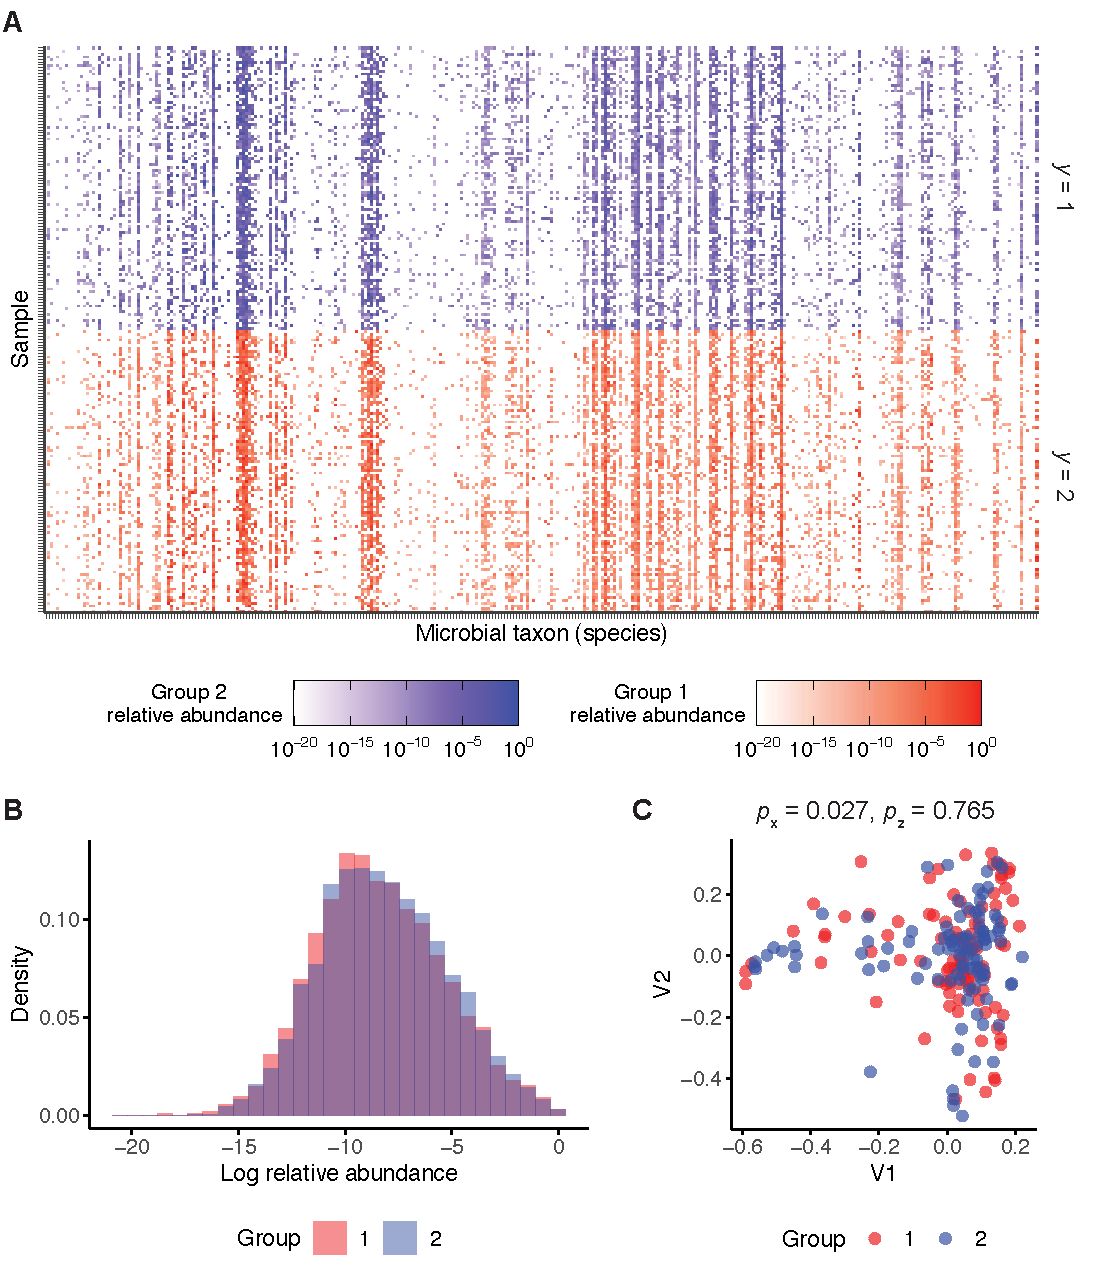
\includegraphics[width=6.5in]{submissions/plos/figures/Fig_S1_rev.pdf}
    \caption[Visualization of a semisynthetic dataset using SparseDOSSA.]{\DIFaddFL{Visualization }\DIFaddendFL of a \DIFdelbeginFL \DIFdelFL{simulated, binary }\DIFdelendFL \DIFaddbeginFL \DIFaddFL{semisynthetic }\DIFaddendFL dataset \DIFdelbeginFL \DIFdelFL{used in this study}\DIFdelendFL \DIFaddbeginFL \DIFaddFL{using SparseDOSSA}\DIFaddendFL . \DIFdelbeginFL \DIFdelFL{Axes }\DIFdelendFL \DIFaddbeginFL \DIFaddFL{(A) Heatmap }\DIFaddendFL of \DIFdelbeginFL \DIFdelFL{each plot correspond to orthonormal vectors that were obtained through eigendecomposition }\DIFdelendFL \DIFaddbeginFL \DIFaddFL{its log-scaled relative abundance by its microbial taxa and sample number. (B) Density histogram }\DIFaddendFL of the \DIFdelbeginFL \DIFdelFL{design matrix $\mathbf{X}$. Alignment on the axis v1 indicates that the samples have been normalized }\DIFdelendFL \DIFaddbeginFL \DIFaddFL{data and }\DIFaddendFL (\DIFdelbeginFL \DIFdelFL{Eq 9, main text}\DIFdelendFL \DIFaddbeginFL \DIFaddFL{C}\DIFaddendFL ) \DIFdelbeginFL \DIFdelFL{. Denoted }\DIFdelendFL \DIFaddbeginFL \DIFaddFL{principal coordinates analysis (PCoA) and PERMANOVA $p$-values based on PCoA results }\DIFaddendFL with \DIFdelbeginFL \DIFdelFL{different colors }\DIFdelendFL \DIFaddbeginFL \DIFaddFL{Euclidean distance ($p_\mathbf{z}$) }\DIFaddendFL and \DIFdelbeginFL \DIFdelFL{shapes are two groups that follow truncated normal distributions }\DIFdelendFL \DIFaddbeginFL \DIFaddFL{original structure }\DIFaddendFL with \DIFdelbeginFL \DIFdelFL{different means but the same covariance }\DIFdelendFL \DIFaddbeginFL \DIFaddFL{Bray-Curtis dissimilarity }\DIFaddendFL (\DIFdelbeginFL \DIFdelFL{Eq 8,main text.}\DIFdelendFL \DIFaddbeginFL \DIFaddFL{$p_\mathbf{x}$}\DIFaddendFL )\DIFaddbeginFL \DIFaddFL{. $N=200$ samples were generated as described.}\DIFaddendFL }
    \DIFdelbeginFL %DIFDELCMD < \label{fig:sim_data_2d}
%DIFDELCMD < %%%
\DIFdelendFL \DIFaddbeginFL \label{fig:sim_data_vis}
\DIFaddendFL \end{figure}
\clearpage

\DIFaddbegin \begin{figure}[h!]
    \centering
    \includegraphics[width=6.5in]{submissions/plos/figures/Fig_S2_rev.pdf}
    \caption[PERMANOVA $p$-values from $F$-informed MDS representations using semisynthetic data.]{\DIFaddFL{PERMANOVA $p$-values from $F$-informed MDS representations using semisynthetic data. $p$-values were plotted against the number of $F$-MDS training epochs for every hyperparameter $\lambda$. Triplicate datasets with size $N=50,100,200,500$ were evaluated. Once $p_\mathbf{z}$ reached to 1 during iteration, the majorization operation was discontinued (e.g., replicate 3 with $N=50$, $\lambda = 0.04$).}}
    \label{fig:sim_fmds_track}
\end{figure}
\clearpage

\DIFaddend \begin{figure}
    \centering
    \DIFdelbeginFL %DIFDELCMD < 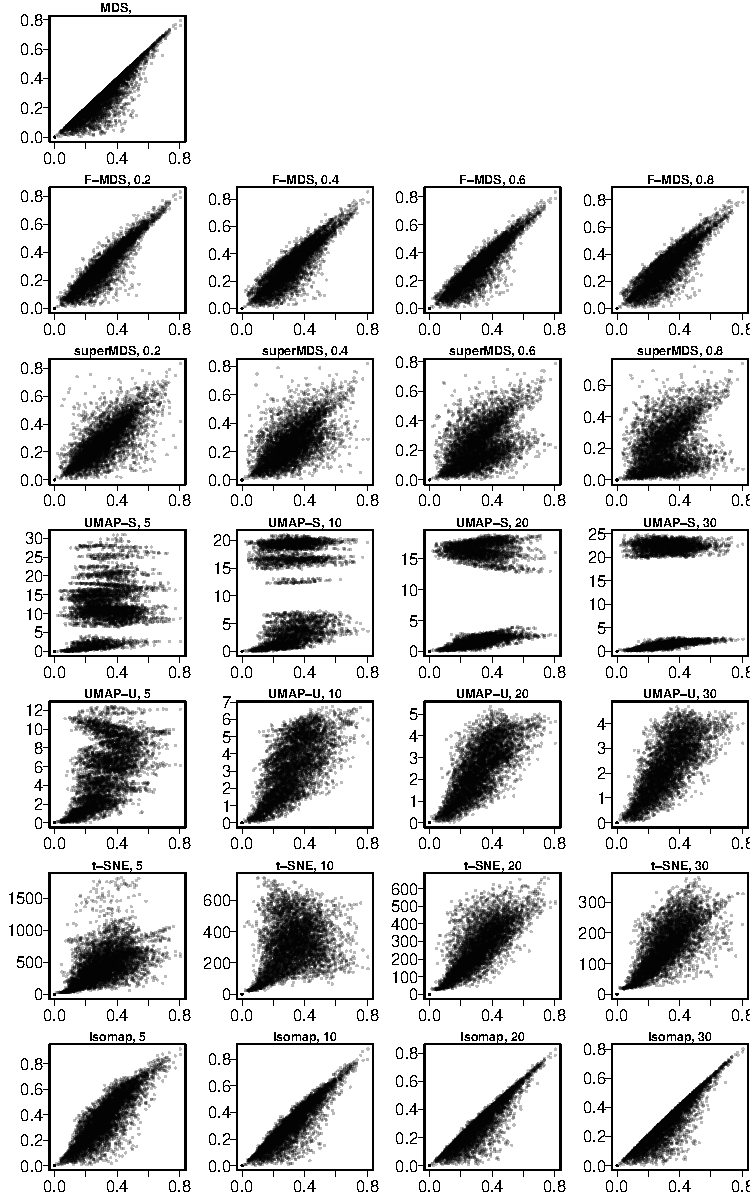
\includegraphics[width=5in]{submissions/plos/figures/Fig_S2.pdf}
%DIFDELCMD <     \caption[Shepard plot from 4D simulated dataset with seven ordination methods.]{%%%
\DIFdelFL{Shepard plot of simulated dataset (first replicate) }\DIFdelendFL \DIFaddbeginFL \includegraphics[width=6.5in]{submissions/plos/figures/Fig_S3_rev.pdf}
    \caption[Pairwise distance analyses from $F$-informed MDS and supervised MDS.]{\DIFaddFL{Pairwise distance analyses from $F$-informed MDS and supervised MDS }\DIFaddendFL using \DIFdelbeginFL \DIFdelFL{seven dimension reduction methods}\DIFdelendFL \DIFaddbeginFL \DIFaddFL{semisynthetic data}\DIFaddendFL . The plots are titled with the \DIFdelbeginFL \DIFdelFL{respective method }\DIFdelendFL \DIFaddbeginFL \DIFaddFL{dataset size $N$ }\DIFaddendFL and \DIFaddbeginFL \DIFaddFL{compared across different methods with }\DIFaddendFL hyperparameter values as follows: $\lambda$, $F$-MDS; $\alpha$, superMDS\DIFdelbeginFL \DIFdelFL{; Nearest neighbors number, supervised }\DIFdelendFL \DIFaddbeginFL \DIFaddFL{. After calculating pairwise distances with Bray-Curtis dissimilarity }\DIFaddendFL (\DIFdelbeginFL \DIFdelFL{-S}\DIFdelendFL \DIFaddbeginFL \DIFaddFL{original}\DIFaddendFL ) \DIFdelbeginFL \DIFdelFL{or unsupervised }\DIFdelendFL \DIFaddbeginFL \DIFaddFL{and Euclidean }\DIFaddendFL (\DIFdelbeginFL \DIFdelFL{-U}\DIFdelendFL \DIFaddbeginFL \DIFaddFL{2D representation}\DIFaddendFL )\DIFdelbeginFL \DIFdelFL{UMAP; Perplexity}\DIFdelendFL , \DIFdelbeginFL \DIFdelFL{t-SNE; Shortest dissimilarities number, Isomap. X- }\DIFdelendFL \DIFaddbeginFL \DIFaddFL{(B) their Pearson correlation coefficient }\DIFaddendFL and \DIFdelbeginFL \DIFdelFL{Y-axis denote the pairwise distance in the original and embedding dimensions, respectively}\DIFdelendFL \DIFaddbeginFL \DIFaddFL{(C) normalized stress (Stress-1) were obtained}\DIFaddendFL . \DIFaddbeginFL \DIFaddFL{Error bars are standard deviation of triplicates.}\DIFaddendFL }
    \DIFdelbeginFL %DIFDELCMD < \label{fig:shepard_sim_all}
%DIFDELCMD < %%%
\DIFdelendFL \DIFaddbeginFL \label{fig:sim_fmds_smds}
\DIFaddendFL \end{figure}
\clearpage

\begin{figure}
    \centering
    \DIFdelbeginFL %DIFDELCMD < \includegraphics[width=5in]{submissions/plos/figures/Fig_S3.pdf}
%DIFDELCMD <     \caption[\textit{F}-correlation plot from simulated dataset.]{%%%
\textit{\DIFdelFL{F}}%DIFAUXCMD
\DIFdelFL{-correlation plot with simulated data. Pseudo }\DIFdelendFL \DIFaddbeginFL \includegraphics[width=6.5in]{submissions/plos/figures/Fig_S4_rev_gridsearch.pdf}
    \caption[Hyperparameter selection using grid search.]{\DIFaddFL{Hyperparameter selection for }\DIFaddendFL $F$\DIFdelbeginFL \DIFdelFL{-ratios were calculated in }\DIFdelendFL \DIFaddbeginFL \DIFaddFL{-informed MDS using grid search. An objective function $f_{\rm obj}(\lambda)$ was defined to simultaneously reflect }\DIFaddendFL the \DIFaddbeginFL \DIFaddFL{number of training epochs and the preservation of the }\DIFaddendFL original \DIFdelbeginFL \DIFdelFL{dimension }\DIFdelendFL \DIFaddbeginFL \DIFaddFL{structure }\DIFaddendFL (\DIFdelbeginFL \DIFdelFL{x-axis}\DIFdelendFL \DIFaddbeginFL \DIFaddFL{see Equation \ref{eq:def_grid_search}}\DIFaddendFL )\DIFdelbeginFL \DIFdelFL{and in each dimension reduction method }\DIFdelendFL \DIFaddbeginFL \DIFaddFL{. }\DIFaddendFL (\DIFdelbeginFL \DIFdelFL{y-axis}\DIFdelendFL \DIFaddbeginFL \DIFaddFL{A}\DIFaddendFL ) \DIFdelbeginFL \DIFdelFL{using first replicate of the simulated }\DIFdelendFL \DIFaddbeginFL \DIFaddFL{For each semisynthetic }\DIFaddendFL dataset \DIFdelbeginFL \DIFdelFL{. Pseudo $F$'s were calculated by randomly permuting labels by 500 times. Highlighted with red denotes }\DIFdelendFL \DIFaddbeginFL \DIFaddFL{size $N$, $f_{\rm obj}(\lambda)$ is plotted against }\DIFaddendFL the \DIFdelbeginFL \DIFdelFL{location }\DIFdelendFL \DIFaddbeginFL \DIFaddFL{hyperparameter $\lambda$. The minimum value }\DIFaddendFL of \DIFdelbeginFL \DIFdelFL{$F$'s from unpermuted labels}\DIFdelendFL \DIFaddbeginFL \DIFaddFL{$f_{\rm obj}(\lambda)$ is highlighted in red}\DIFaddendFL . \DIFdelbeginFL \DIFdelFL{Each plot }\DIFdelendFL \DIFaddbeginFL \DIFaddFL{(B) The optimal hyperparameter $\lambda_{\rm min}$ }\DIFaddendFL is \DIFdelbeginFL \DIFdelFL{titled }\DIFdelendFL \DIFaddbeginFL \DIFaddFL{plotted against dataset size $N$, }\DIFaddendFL with \DIFdelbeginFL \DIFdelFL{the method and hyperparameter used}\DIFdelendFL \DIFaddbeginFL \DIFaddFL{each dataset represented by a symbol}\DIFaddendFL .}
    \DIFdelbeginFL %DIFDELCMD < \label{fig:f_corr_sim_all}
%DIFDELCMD < %%%
\DIFdelendFL \DIFaddbeginFL \label{fig:fmds_gridsearch}
\DIFaddendFL \end{figure}
\clearpage

\begin{figure}
    \centering
    \DIFdelbeginFL %DIFDELCMD < \includegraphics[width=5in]{submissions/plos/figures/Fig_S4.pdf}
%DIFDELCMD <     %%%
%DIFDELCMD < \caption[Shepard plot from algal microbiome dataset with eight ordination methods.]{%
{%DIFAUXCMD
\DIFdelFL{Shepard plot of algal-associated bacterial community data using eight dimension reduction methods. The plots are titled with the respective method and hyperparameter values as follows: $\lambda$, $F$-MDS; $\alpha$, superMDS; Nearest neighbors number, supervised (-S) or unsupervised (-U) UMAP; Perplexity, t-SNE; Shortest dissimilarities number, Isomap; none, neural network (NN). X- and Y-axis denote distances in the original and embedding dimensions, respectively.}}
    %DIFAUXCMD
%DIFDELCMD < \label{fig:shepard_alga_all}
%DIFDELCMD < %%%
\DIFdelendFL \DIFaddbeginFL \includegraphics[width=5.05in]{submissions/plos/figures/Fig_S5_rev.pdf}
    \caption[Comparison of quality metrics of benchmark ordination methods.]{\DIFaddFL{Comparison of quality metrics of ordination methods evaluated on semisynthetic datasets. Trustworthiness and continuity to evaluate (A) Local structural preservation is assessed using trustworthiness and continuity. (B) Global structural preservation is similarly evaluated with trustworthiness and continuity. (C) Global distortion is quantified by Stress-1 and Pearson correlation of Shepard diagrams. (D) Preservation of statistical inference is measured by the $F$-rank-ratio and $F$-correlation using randomly permuted label sets. The following hyperparameters were used for each method: $\lambda$ for $F$-MDS, number of neighbors $n$ for UMAP (both supervised (-S) and unsupervised (-U)), perplexity (perp) for t-SNE, and the number of shortest dissimilarities $n$ for Isomap. Error bars represent the standard deviation across triplicate measurements.}}
    \label{fig:sim_eval_all}
\DIFaddendFL \end{figure}
\clearpage

\begin{figure}
    \centering
    \DIFdelbeginFL %DIFDELCMD < \includegraphics[width=5in]{submissions/plos/figures/Fig_S5.pdf}
%DIFDELCMD <     %%%
%DIFDELCMD < \caption[\textit{F}-correlation plot from algal microbiome dataset.]{%
{%DIFAUXCMD
\textit{\DIFdelFL{F}}%DIFAUXCMD
\DIFdelFL{-correlation plot from algal microbiome dataset. Pseudo $F$-ratios comparing the original dimension (x-axis) and from eight dimension reduction methods (y-axis) with algal microbiome data. Pseudo $F$'s were calculated by randomly permuting labels by 500 times. Highlighted with red denotes the location of $F$'s from unpermuted labels. Each plot is titled with the method and hyperparameter used.}}
    %DIFAUXCMD
%DIFDELCMD < \label{fig:f_corr_alga_all}
%DIFDELCMD < %%%
\DIFdelendFL \DIFaddbeginFL \includegraphics[width=5in]{submissions/plos/figures/Fig_S6_rev.pdf}
    \caption[Shepard plot from algal microbiome dataset with eight ordination methods.]{\DIFaddFL{Shepard plot of algal-associated bacterial community data using eight dimension reduction methods. The plots are titled with the respective method and hyperparameter values as follows: $\lambda$, $F$-MDS; $\alpha$, superMDS; Nearest neighbors number, supervised (-S) or unsupervised (-U) UMAP; Perplexity, t-SNE; Shortest dissimilarities number, Isomap; none, neural network (NN). X- and Y-axis denote distances in the original and embedding dimensions, respectively.}}
    \label{fig:shepard_alga_all}
\DIFaddendFL \end{figure}
\clearpage

\begin{figure}
    \centering
    \DIFdelbeginFL %DIFDELCMD < \includegraphics[width=6.5in]{submissions/plos/figures/Fig_S6.pdf}
%DIFDELCMD <     \caption[Pairs plot of simulated, trinary data.]{%%%
\DIFdelFL{Pairs plot of trinary, four-dimensional simulated data. Each row and column corresponds to respective axis for the projection. Denoted with different colors or shapes are the trinary groups that follow normal distributions with different means but the same covariance (Eq 10, main text.) }%DIFDELCMD < \MBLOCKRIGHTBRACE
%DIFDELCMD <     \label{fig:sim_data_4d}
%DIFDELCMD < %%%
\DIFdelendFL \DIFaddbeginFL \includegraphics[width=5in]{submissions/plos/figures/Fig_S7_rev.pdf}
    \caption[\textit{F}-correlation plot from algal microbiome dataset.]{\textit{\DIFaddFL{F}}\DIFaddFL{-correlation plot from algal microbiome dataset. Pseudo $F$-ratios comparing the original dimension (x-axis) and from eight dimension reduction methods (y-axis) with algal microbiome data. Pseudo $F$'s were calculated by randomly permuting labels by 500 times. Highlighted with red denotes the location of $F$'s from unpermuted labels. Each plot is titled with the method and hyperparameter used.}}
    \label{fig:f_corr_alga_all}
\DIFaddendFL \end{figure}
\clearpage

\begin{figure}
    \centering
    \DIFdelbeginFL %DIFDELCMD < \includegraphics[width=6.5in]{submissions/plos/figures/Fig_S7.pdf}
%DIFDELCMD <     %%%
\DIFdelendFL \DIFaddbeginFL \includegraphics[width=6.5in]{submissions/plos/figures/Fig_S8_rev.pdf}
    \DIFaddendFL \caption[Cluster centroid and variances of $F$-MDS representations.]{Cluster \DIFdelbeginFL \DIFdelFL{centroid }\DIFdelendFL \DIFaddbeginFL \DIFaddFL{centroids }\DIFaddendFL and variances of $F$-MDS representations \DIFaddbeginFL \DIFaddFL{are shown }\DIFaddendFL for \DIFdelbeginFL \DIFdelFL{simulated dataset }\DIFdelendFL \DIFaddbeginFL \DIFaddFL{semisynthetic datasets of size $N=50$ }\DIFaddendFL (\DIFdelbeginFL \DIFdelFL{A-C}\DIFdelendFL \DIFaddbeginFL \DIFaddFL{A–C}\DIFaddendFL )\DIFaddbeginFL \DIFaddFL{, $N=100$ (D–F), $N=200$ (G–I), $N=500$ (J–L) }\DIFaddendFL and \DIFaddbeginFL \DIFaddFL{for the }\DIFaddendFL algal microbiome (\DIFdelbeginFL \DIFdelFL{D-F}\DIFdelendFL \DIFaddbeginFL \DIFaddFL{M–O}\DIFaddendFL ). \DIFdelbeginFL \DIFdelFL{A,D: Distance }\DIFdelendFL \DIFaddbeginFL \DIFaddFL{The first column in each row displays the distance }\DIFaddendFL between group centroids. \DIFdelbeginFL \DIFdelFL{B,E: Variance }\DIFdelendFL \DIFaddbeginFL \DIFaddFL{The second and third columns show the variance }\DIFaddendFL of each group\DIFdelbeginFL \DIFdelFL{measured in its long-axis. C}\DIFdelendFL , \DIFdelbeginFL \DIFdelFL{F: Variance of each group }\DIFdelendFL measured \DIFdelbeginFL \DIFdelFL{in its short-axis}\DIFdelendFL \DIFaddbeginFL \DIFaddFL{along the long and short principal axes, respectively}\DIFaddendFL . For \DIFdelbeginFL \DIFdelFL{simulated dataset error bars denote standard deviation of triplicates. For }\DIFdelendFL \DIFaddbeginFL \DIFaddFL{the }\DIFaddendFL variance \DIFdelbeginFL \DIFdelFL{calculations}\DIFdelendFL \DIFaddbeginFL \DIFaddFL{panels}\DIFaddendFL , blue and red colors denote \DIFdelbeginFL \DIFdelFL{group }\DIFdelendFL \DIFaddbeginFL \DIFaddFL{groups }\DIFaddendFL 1 and \DIFdelbeginFL \DIFdelFL{2, respectively}\DIFdelendFL \DIFaddbeginFL \DIFaddFL{2. Error bars represent the standard deviation across triplicate measurements}\DIFaddendFL .}
    \label{fig:fmds_rep_analysis}
\end{figure}
\clearpage

%DIF <  \begin{figure}
%DIF <      \centering
%DIF <      \includegraphics[width=6.5in]{submissions/nips/figures/site-config-all.pdf}
%DIF <      \caption[Visualization of bacterial community using FMDS.]{Visualization of bacterial community using proposed FMDS. Microbial community samples are collected from Site 1 (top row) and Site 2 (bottom row).}
%DIF <      \label{fig:site_config_all}
%DIF <  \end{figure}
%DIF <  \clearpage
\DIFdelbegin %DIFDELCMD < 

%DIFDELCMD < %%%
%DIF <  \begin{figure}
%DIF <      \centering
%DIF <      \includegraphics[width=6.5in]{submissions/nips/figures/shepard_site.png}
%DIF <      \caption[Shepard plot of community dataset.]{Shepard plot in microbial community data collected from site 1 (first row) and site 2 (second row) for a range of hyperparameters.}
%DIF <      \label{fig:shepard_site}
%DIF <  \end{figure}
%DIF <  \clearpage
%DIFDELCMD < 

%DIFDELCMD < %%%
%DIF <  \begin{figure}
%DIF <      \centering
%DIF <      \includegraphics[width=6.5in]{submissions/ISMB/figures/cirrhosis.pdf}
%DIF <      \caption[Visualization of cirrhosis patients and healthy human gut microbiome.]{Visualization of cirrhosis patients and healthy human gut microbiome. The following hyperparameters were used: $\lambda=0.3$ (FMDS), neighbors $=10$ (UMAP-S), neighbors $=30$ (UMAP-U), perplexity$=7$ (t-SNE), $K=10$ (Isomap).}
%DIF <      \label{fig:cirr}
%DIF <  \end{figure}
%DIF <  \clearpage
\DIFdelend \DIFaddbegin \begin{figure}
    \centering
    \includegraphics[width=6.5in]{submissions/plos/figures/Fig_S9_rev.pdf}
    \caption[Visualization of a semisynthetic ternary dataset.]{\DIFaddFL{Visualization of a semisynthetic ternary dataset. (A) Heatmap of its log-scaled relative abundance by its microbial taxa and sample number. (B) Density histogram of the data and (C) principal coordinates analysis (PCoA) and PERMANOVA $p$-values based on PCoA results with Euclidean distance ($p_\mathbf{z}$) and original structure with Bray-Curtis dissimilarity ($p_\mathbf{x}$). $N=75$ semisynthetic data were generated.}}
    \label{fig:sim_ternary_vis}
\end{figure}
\clearpage
\DIFaddend 


\begin{singlespace}
\bibliographystyle{acm}
\documentclass[11pt]{article}
%DIF LATEXDIFF DIFFERENCE FILE


%%%%%%%%%%%%%%%%%%%%%%%%%%%%%%%%%%%%%%%%%%%%%%%%%%%%%%%%%
%%%%%%%%%%%%%%%%%%%%%%%%% Setup %%%%%%%%%%%%%%%%%%%%%%%%%
\usepackage[margin=1in]{geometry}
\usepackage{fmtcount} % 1st, 2nd...
\usepackage[english]{babel}
\usepackage{soul} % spacing
\usepackage{enumerate} % change enum label
\usepackage{framed} % frame pagebreak
\usepackage{authblk}
\usepackage{setspace}
\usepackage{tocloft}

%%%%% Math, Code 
\usepackage{amsmath}
\usepackage{amsfonts}
\usepackage{amssymb}
\usepackage{amsthm}
\usepackage{amscd}
\usepackage{array}
\usepackage{mathtools} 
\usepackage{verbatim}
\usepackage{fancyvrb} % verbatim
\usepackage{algpseudocode}
\usepackage{algorithm}

%%%%% Graphic, Figure, Table
\usepackage{graphicx}
\usepackage{epstopdf}
\usepackage{xcolor}
\usepackage[labelsep=none]{caption}
\usepackage{subcaption}
\usepackage{multirow} % table
\usepackage{longtable} % table to next page
\usepackage{rotating}
\usepackage{wrapfig} % wrap fig, tbl with text

%%%%% Bib, Cite
\usepackage{url}
\usepackage{cite}
\usepackage{fancyref}
\usepackage{hyperref}
\hypersetup{linktocpage}

%%%%%% Setup
% \captionsetup{compatibility=false} %subfig
% \DeclareCaptionLabelFormat{Sformat}{S#2 #1}
% \captionsetup[figure]{labelformat=Sformat}
% \captionsetup[table]{labelformat=Sformat}
\hypersetup{colorlinks=false}
\setlength{\parskip}{0.5em}

\newtheorem{thm}{Theorem}[section]
\newtheorem{cor}[thm]{Corollary}
\newtheorem{lem}[thm]{Lemma}
\newtheorem{prop}[thm]{Proposition}
\newtheorem{dfn}{Definition}
\newtheorem{ex}{Example}
\newtheorem{cmt}{Cmt}[section]
\newtheorem{rmk}{Remark}[section]
\newcommand{\rb}[1]{\raisebox{-.5em}[0pt]{#1}}
\newcommand{\1}{{\rm 1}\kern-0.24em{\rm I}}
\newcommand{\cN}{\mathcal{N}}
\newcommand{\cO}{\mathcal{O}}
\renewcommand{\mid}{\, | \ , }
\makeatletter
\renewcommand\theequation{S\@arabic\c@equation}
\makeatother

\renewcommand\Affilfont{\normalsize}
% \renewcommand{\baselinestretch}{1.3}

\DeclareMathOperator*{\argmin}{arg\,min}
\DeclareMathOperator*{\argmax}{arg\,max}
\DeclareMathOperator*{\bbr}{\mathbb{R}}
%%%%%%%%%%%%%%%%%%%%%%%%%%%%%%%%%%%%%%%%%%%%%%%%%%%%%%%
%%%%%%%%%%%%%%%%%%%%%%%%%%%%%%%%%%%%%%%%%%%%%%%%%%%%%%%

\title{Supporting Information of ``Multidimensional scaling informed by $F$-statistic: Visualizing grouped microbiome data with inference''}
\author[1\dag]{Hyungseok Kim}
\author[2\dag]{Soobin Kim}
\author[3]{Jeffrey A. Kimbrel}
\author[3]{Megan M. Morris}
\author[3]{Xavier Mayali}
\author[1$*$]{Cullen R. Buie}
\affil[1]{Massachusetts Institute of Technology, Cambridge, MA, USA}
\affil[2]{University of California, Davis, Davis, CA, USA}
\affil[3]{Lawrence Livermore National Laboratory, Livermore, CA, USA}
\affil[$\dagger$] {These authors contributed equally to this work.}
\affil[$^*$]{Correspondence: crb@mit.edu.}
% \author{}
\date{}
%DIF PREAMBLE EXTENSION ADDED BY LATEXDIFF
%DIF UNDERLINE PREAMBLE %DIF PREAMBLE
\RequirePackage[normalem]{ulem} %DIF PREAMBLE
\RequirePackage{color}\definecolor{RED}{rgb}{1,0,0}\definecolor{BLUE}{rgb}{0,0,1} %DIF PREAMBLE
\providecommand{\DIFaddtex}[1]{{\protect\color{blue}\uwave{#1}}} %DIF PREAMBLE
\providecommand{\DIFdeltex}[1]{{\protect\color{red}\sout{#1}}}                      %DIF PREAMBLE
%DIF SAFE PREAMBLE %DIF PREAMBLE
\providecommand{\DIFaddbegin}{} %DIF PREAMBLE
\providecommand{\DIFaddend}{} %DIF PREAMBLE
\providecommand{\DIFdelbegin}{} %DIF PREAMBLE
\providecommand{\DIFdelend}{} %DIF PREAMBLE
\providecommand{\DIFmodbegin}{} %DIF PREAMBLE
\providecommand{\DIFmodend}{} %DIF PREAMBLE
%DIF FLOATSAFE PREAMBLE %DIF PREAMBLE
\providecommand{\DIFaddFL}[1]{\DIFadd{#1}} %DIF PREAMBLE
\providecommand{\DIFdelFL}[1]{\DIFdel{#1}} %DIF PREAMBLE
\providecommand{\DIFaddbeginFL}{} %DIF PREAMBLE
\providecommand{\DIFaddendFL}{} %DIF PREAMBLE
\providecommand{\DIFdelbeginFL}{} %DIF PREAMBLE
\providecommand{\DIFdelendFL}{} %DIF PREAMBLE
%DIF HYPERREF PREAMBLE %DIF PREAMBLE
\providecommand{\DIFadd}[1]{\texorpdfstring{\DIFaddtex{#1}}{#1}} %DIF PREAMBLE
\providecommand{\DIFdel}[1]{\texorpdfstring{\DIFdeltex{#1}}{}} %DIF PREAMBLE
\newcommand{\DIFscaledelfig}{0.5}
%DIF HIGHLIGHTGRAPHICS PREAMBLE %DIF PREAMBLE
\RequirePackage{settobox} %DIF PREAMBLE
\RequirePackage{letltxmacro} %DIF PREAMBLE
\newsavebox{\DIFdelgraphicsbox} %DIF PREAMBLE
\newlength{\DIFdelgraphicswidth} %DIF PREAMBLE
\newlength{\DIFdelgraphicsheight} %DIF PREAMBLE
% store original definition of \includegraphics %DIF PREAMBLE
\LetLtxMacro{\DIFOincludegraphics}{\includegraphics} %DIF PREAMBLE
\newcommand{\DIFaddincludegraphics}[2][]{{\color{blue}\fbox{\DIFOincludegraphics[#1]{#2}}}} %DIF PREAMBLE
\newcommand{\DIFdelincludegraphics}[2][]{% %DIF PREAMBLE
\sbox{\DIFdelgraphicsbox}{\DIFOincludegraphics[#1]{#2}}% %DIF PREAMBLE
\settoboxwidth{\DIFdelgraphicswidth}{\DIFdelgraphicsbox} %DIF PREAMBLE
\settoboxtotalheight{\DIFdelgraphicsheight}{\DIFdelgraphicsbox} %DIF PREAMBLE
\scalebox{\DIFscaledelfig}{% %DIF PREAMBLE
\parbox[b]{\DIFdelgraphicswidth}{\usebox{\DIFdelgraphicsbox}\\[-\baselineskip] \rule{\DIFdelgraphicswidth}{0em}}\llap{\resizebox{\DIFdelgraphicswidth}{\DIFdelgraphicsheight}{% %DIF PREAMBLE
\setlength{\unitlength}{\DIFdelgraphicswidth}% %DIF PREAMBLE
\begin{picture}(1,1)% %DIF PREAMBLE
\thicklines\linethickness{2pt} %DIF PREAMBLE
{\color[rgb]{1,0,0}\put(0,0){\framebox(1,1){}}}% %DIF PREAMBLE
{\color[rgb]{1,0,0}\put(0,0){\line( 1,1){1}}}% %DIF PREAMBLE
{\color[rgb]{1,0,0}\put(0,1){\line(1,-1){1}}}% %DIF PREAMBLE
\end{picture}% %DIF PREAMBLE
}\hspace*{3pt}}} %DIF PREAMBLE
} %DIF PREAMBLE
\LetLtxMacro{\DIFOaddbegin}{\DIFaddbegin} %DIF PREAMBLE
\LetLtxMacro{\DIFOaddend}{\DIFaddend} %DIF PREAMBLE
\LetLtxMacro{\DIFOdelbegin}{\DIFdelbegin} %DIF PREAMBLE
\LetLtxMacro{\DIFOdelend}{\DIFdelend} %DIF PREAMBLE
\DeclareRobustCommand{\DIFaddbegin}{\DIFOaddbegin \let\includegraphics\DIFaddincludegraphics} %DIF PREAMBLE
\DeclareRobustCommand{\DIFaddend}{\DIFOaddend \let\includegraphics\DIFOincludegraphics} %DIF PREAMBLE
\DeclareRobustCommand{\DIFdelbegin}{\DIFOdelbegin \let\includegraphics\DIFdelincludegraphics} %DIF PREAMBLE
\DeclareRobustCommand{\DIFdelend}{\DIFOaddend \let\includegraphics\DIFOincludegraphics} %DIF PREAMBLE
\LetLtxMacro{\DIFOaddbeginFL}{\DIFaddbeginFL} %DIF PREAMBLE
\LetLtxMacro{\DIFOaddendFL}{\DIFaddendFL} %DIF PREAMBLE
\LetLtxMacro{\DIFOdelbeginFL}{\DIFdelbeginFL} %DIF PREAMBLE
\LetLtxMacro{\DIFOdelendFL}{\DIFdelendFL} %DIF PREAMBLE
\DeclareRobustCommand{\DIFaddbeginFL}{\DIFOaddbeginFL \let\includegraphics\DIFaddincludegraphics} %DIF PREAMBLE
\DeclareRobustCommand{\DIFaddendFL}{\DIFOaddendFL \let\includegraphics\DIFOincludegraphics} %DIF PREAMBLE
\DeclareRobustCommand{\DIFdelbeginFL}{\DIFOdelbeginFL \let\includegraphics\DIFdelincludegraphics} %DIF PREAMBLE
\DeclareRobustCommand{\DIFdelendFL}{\DIFOaddendFL \let\includegraphics\DIFOincludegraphics} %DIF PREAMBLE
%DIF END PREAMBLE EXTENSION ADDED BY LATEXDIFF

\begin{document}

\renewcommand*\contentsname{\normalsize List of Supplementary Notes}
\makeatletter
\renewcommand{\tableofcontents}{\@starttoc{toc}}
\renewcommand*\l@section{\@dottedtocline{1}{0em}{6.3em}}
\let\l@table\l@content
\makeatother

\makeatletter
\renewcommand{\listoffigures}{\@starttoc{lof}}
\renewcommand*\l@figure{\@dottedtocline{1}{0em}{3.5em}}
\let\l@table\l@figure
\makeatother

\makeatletter
\renewcommand{\listoftables}{\@starttoc{lot}}
\renewcommand*\l@table{\@dottedtocline{1}{0em}{4.5em}}
\let\l@table\l@table
\makeatother

\renewcommand\thesection{S\arabic{section} Appendix.}
\makeatletter
\renewcommand*{\@seccntformat}[1]{\csname the#1\endcsname\hspace{0.5em}}
\makeatother

\renewcommand{\figurename}{\!\!}
\let\standardthefigure\thefigure
\renewcommand\thefigure{S\standardthefigure\ Fig.\ }
\addtolength{\cftfignumwidth}{15pt}

\renewcommand{\tablename}{\!\!}
\let\standardthetable\thetable
\renewcommand\thetable{S\standardthetable\ Table.\ }

% \renewcommand{\algorithmname}{\!\!}
\let\standardthealgorithm\thealgorithm
\renewcommand\thealgorithm{S\standardthealgorithm}

\maketitle
% \def\thefootnote{\arabic{footnote}}

{\noindent\normalsize\bf List of Supplementary Information}
\tableofcontents
\listoffigures
\listoftables
\clearpage


\section{\DIFdelbegin \DIFdel{Mapping }\DIFdelend \DIFaddbegin \DIFadd{Objective }\DIFaddend function for \DIFaddbegin \DIFadd{computing }\DIFaddend $F$-MDS\DIFdelbegin \DIFdel{.}\DIFdelend } \label{sec:app1}

\DIFdelbegin \DIFdel{In this section, we explain a procedure of deriving a }\DIFdelend \DIFaddbegin \DIFadd{First, we derive a }\DIFaddend mapping function $f_\mathbf{z}(F_\mathbf{x})$ \DIFdelbegin \DIFdel{that is used to minimize }\DIFdelend \DIFaddbegin \DIFadd{for minimizing }\DIFaddend an objective function \DIFdelbegin \DIFdel{for }\DIFdelend \DIFaddbegin \DIFadd{and }\DIFaddend computing $F$-informed MDS.
The \DIFdelbegin \DIFdel{confirmatory term of the objective function (Eq 5 of the main text) is specifically designed }\DIFdelend \DIFaddbegin \DIFadd{mapping function guides }\DIFaddend to minimize a difference in $p$-values testing \DIFdelbegin \DIFdel{for group difference by representations }\DIFdelend \DIFaddbegin \DIFadd{group differences }\DIFaddend under the original $S$- and \DIFdelbegin \DIFdel{two-dimensions}\DIFdelend \DIFaddbegin \DIFadd{two-dimensional embedding through the confirmatory term of the objective (see Eq 5 of the main text)}\DIFaddend .
These \textit{p}-values are obtained from an empirical distribution of the pseudo-$F$s by permuted labels \cite{anderson01} \DIFdelbegin \DIFdel{. 
In other words, by denoting a label set as $[y_i]$ ($i=1,\cdots N$) and its permuted set as $[y_i^\pi]$ with operator $\pi$, we express each }\DIFdelend \DIFaddbegin \DIFadd{(Eq 4, main text). 
For a given label set $[y_i]_{i=1}^{N}$ and its group number $G$, a permuted label set $[y_i^\Pi]_{i=1}^{N}$ and }\DIFaddend $F$\DIFdelbegin \DIFdel{-statistic as
}\DIFdelend \DIFaddbegin \DIFadd{-statistics are expressed as
}\DIFaddend \begin{equation}
\DIFdelbegin %DIFDELCMD < \begin{aligned}
%DIFDELCMD < F^\pi_\mathbf{x} &= 
%DIFDELCMD < \left(\frac{\sum_{i,j}d_{ij}^2}{2\sum_{i,j}d_{ij}^2\,\1\{y_i^\pi = y_j^\pi\}} -1 \right) \cdot (N-2), \\
%DIFDELCMD < F^\pi_\mathbf{z} &= 
%DIFDELCMD < \left(\frac{\sum_{i,j}\|\mathbf{z}_i - \mathbf{z}_j\|_2^2}{2\sum_{i,j}\|\mathbf{z}_i - \mathbf{z}_j\|_2^2\,\1\{y_i^\pi = y_j^\pi\}} -1 \right) \cdot (N-2).
%DIFDELCMD < \label{eq:map1}
%DIFDELCMD < \end{aligned}%%%
\DIFdelend \DIFaddbegin \begin{aligned}
F^\Pi_\mathbf{x} &= 
\left(\frac{\sum_{i,j}d_{ij}^2}{G \sum_{i,j}d_{ij}^2\,\1\{y_i^\Pi = y_j^\Pi\}} -1 \right) \cdot \frac{N-G}{G-1}, \\
F^\Pi_\mathbf{z} &= 
\left(\frac{\sum_{i,j}\|\mathbf{z}_i - \mathbf{z}_j\|_2^2}{G\sum_{i,j}\|\mathbf{z}_i - \mathbf{z}_j\|_2^2\,\1\{y_i^\Pi = y_j^\Pi\}} -1 \right) \cdot \frac{N-G}{G-1}.
\label{eq:map1}
\end{aligned}\DIFaddend 
\end{equation}
% \end{align} 

It should be noted that the pseudo $F$-ratios can range differently based on how the samples are projected onto 2D. To scale between these two ratios and minimize the difference in $p$-values, we consider a mapping $f_\mathbf{z}: F_\mathbf{x} \rightarrow F_\mathbf{z}$ from a pair of ratios \DIFdelbegin \DIFdel{$(F_\mathbf{x}^{\pi_1}, F_\mathbf{z}^{\pi_2})$ }\DIFdelend \DIFaddbegin \DIFadd{$(F_\mathbf{x}^{\Pi_1}, F_\mathbf{z}^{\Pi_2})$ }\DIFaddend where each element was ordered from two independent sets of repeated permutations. Figure below exemplifies how the $F$-ratios at each dimensionality scaled differently and depended on the choice of hyperparameter $\lambda$. In both settings, the $F$-ratio in $S$-dimension ranged \DIFdelbegin \DIFdel{between zero and six }\DIFdelend \DIFaddbegin \DIFadd{in }[\DIFadd{0,6}] \DIFaddend whereas in 2D representation the ratio ranged in [0,4]. The hyperparameter, however, impacted the detailed relationship between ordered $F_\mathbf{x}$ and ordered $F_\mathbf{x}$, when compared to each other. 

\begin{figure}[h]
    \centering
    \includegraphics[width=5.5in]{submissions/plos/figures/supp-mds_Fval.pdf}
    \caption*{Figure: Mapping pseudo-$F$'s between two dimensionalities. Each $F_\mathbf{x} \text{-} F_\mathbf{z}$ relationship was obtained by permuting labels over 1,000 times, and by setting a hyperparameter $\lambda$ that is used to perform the majorization.}
    \label{fig:mds-fval}
\end{figure}

Using the mapping function $f_\mathbf{z}$, we \DIFdelbegin \DIFdel{now }\DIFdelend derive an exact \DIFdelbegin \DIFdel{form of confirmatory term proposed }\DIFdelend \DIFaddbegin \DIFadd{expression for the confirmatory term introduced }\DIFaddend in the $F$-MDS objective function\DIFdelbegin \DIFdel{(Eq 5 of main text)}\DIFdelend . The proposed form $\left|F_\mathbf{z} - f_\mathbf{z}(F_\mathbf{x})\right|$ measures how \DIFaddbegin \DIFadd{accurately }\DIFaddend the 2D representation \DIFdelbegin \DIFdel{accurately reflected }\DIFdelend \DIFaddbegin \DIFadd{reflects }\DIFaddend the $S$-dimensional distance structure \DIFdelbegin \DIFdel{with respect to }\DIFdelend \DIFaddbegin \DIFadd{regarding }\DIFaddend the sample labels. \DIFdelbegin \DIFdel{Having the }\DIFdelend \DIFaddbegin \DIFadd{A }\DIFaddend difference close to zero indicates that no \DIFdelbegin \DIFdel{additional update with the representation is required (let us denote it as }\DIFdelend \DIFaddbegin \DIFadd{further updates to the representation are required (denoted }\DIFaddend $\mathbf{Z}^*$). \DIFdelbegin \DIFdel{Now by substituting }\DIFdelend \DIFaddbegin \DIFadd{Substituting }\DIFaddend the confirmatory term $\left|F_\mathbf{z} - f_\mathbf{z}(F_\mathbf{x})\right|$ with Equation \ref{eq:map1}, we define \DIFdelbegin \DIFdel{$\1\{y_i^\pi = y_j^\pi\}\coloneqq\epsilon_{ij}$ and write
}\DIFdelend \DIFaddbegin \DIFadd{$\epsilon_{ij}\coloneqq\1\{y_i^\Pi = y_j^\Pi\}$ and write
}\DIFaddend \begin{align}
\mathbf{Z}^* &= \argmin_\mathbf{Z}\,\left|F_\mathbf{z} - f_\mathbf{z}(F_\mathbf{x})\right| \\
& = \argmin_\mathbf{Z}\,\left|\DIFdelbegin \DIFdel{(N-2)}\DIFdelend \DIFaddbegin \DIFadd{\frac{N-G}{G-1}}\DIFaddend \cdot\left(\DIFdelbegin \DIFdel{\frac{\sum_{i,j}\|\mathbf{z}_i - \mathbf{z}_j\|_2^2}{2\sum_{i,j}\epsilon_{ij}\|\mathbf{z}_i - \mathbf{z}_j\|_2^2} }\DIFdelend \DIFaddbegin \DIFadd{\frac{\sum_{i,j}\|\mathbf{z}_i - \mathbf{z}_j\|_2^2}{G\sum_{i,j}\epsilon_{ij}\|\mathbf{z}_i - \mathbf{z}_j\|_2^2} }\DIFaddend -1 \right) - f_\mathbf{z}(F_\mathbf{x})\right| \\
&= \argmin_\mathbf{Z}\,\left|\DIFdelbegin \DIFdel{\frac{\sum_{i,j}\|\mathbf{z}_i - \mathbf{z}_j\|_2^2}{2\sum_{i,j}\epsilon_{ij}\|\mathbf{z}_i - \mathbf{z}_j\|_2^2} }\DIFdelend \DIFaddbegin \DIFadd{\frac{\sum_{i,j}\|\mathbf{z}_i - \mathbf{z}_j\|_2^2}{G\sum_{i,j}\epsilon_{ij}\|\mathbf{z}_i - \mathbf{z}_j\|_2^2} }\DIFaddend -1 - \DIFdelbegin \DIFdel{\frac{f_\mathbf{z}(F_\mathbf{x})}{N-2} }\DIFdelend \DIFaddbegin \DIFadd{\frac{G-1}{N-G}\cdot{f_\mathbf{z}(F_\mathbf{x})} }\DIFaddend \right| \DIFdelbegin %DIFDELCMD < \\
%DIFDELCMD < &%%%
\DIFdel{= \argmin_\mathbf{Z}\,}%DIFDELCMD < \left| %%%
\DIFdel{\frac{\sum_{i,j}\|\mathbf{z}_i - \mathbf{z}_j\|_2^2 - 2\sum_{i,j}\epsilon_{ij}\|\mathbf{z}_i - \mathbf{z}_j\|_2^2 \cdot [1+f_\mathbf{z}(F_\mathbf{x})/(N-2)]}{2\sum_{i,j}\epsilon_{ij}\|\mathbf{z}_i - \mathbf{z}_j\|_2^2} }%DIFDELCMD < \right| %%%
\DIFdelend \label{eq:pre_approx}\\
&\approx \argmin_\mathbf{Z}\,\left| \sum_{i,j}\|\mathbf{z}_i - \mathbf{z}_j\|_2^2 - \DIFdelbegin \DIFdel{2}\DIFdelend \DIFaddbegin \DIFadd{G}\DIFaddend \sum_{i,j}\epsilon_{ij}\|\mathbf{z}_i - \mathbf{z}_j\|_2^2 \cdot \left(1+\DIFdelbegin \DIFdel{\frac{f_\mathbf{z}(F_\mathbf{x})}{N-2}}\DIFdelend \DIFaddbegin \DIFadd{\frac{G-1}{N-G}\cdot{f_\mathbf{z}(F_\mathbf{x})}}\DIFaddend \right) \right| \label{eq:approx}\\
&= \argmin_\mathbf{Z}\,\left|\sum_{i,j} \left[1- \DIFdelbegin \DIFdel{2}\DIFdelend \DIFaddbegin \DIFadd{G}\DIFaddend \epsilon_{ij} \left(1+\DIFdelbegin \DIFdel{\frac{f_\mathbf{z}(F_\mathbf{x})}{N-2}}\DIFdelend \DIFaddbegin \DIFadd{\frac{G-1}{N-G}\cdot{f_\mathbf{z}(F_\mathbf{x})}}\DIFaddend \right)\right] \|\mathbf{z}_i - \mathbf{z}_j\|_2^2\right| \DIFaddbegin \label{eq:pre_conf}\DIFaddend ,
\end{align}
where Equation \ref{eq:approx} \DIFdelbegin \DIFdel{is approximated from Equation \ref{eq:pre_approx} }\DIFdelend \DIFaddbegin \DIFadd{follows from the numerator of Equation \ref{eq:pre_approx}. 
}

\DIFadd{Finally, the exact $F$-MDS confirmatory term is derived through a scaling analysis of expression \ref{eq:pre_conf} by comparing its value to that of the raw stress (main text Eq 1). Binary semisynthetic datasets generated by SparseDOSSA \mbox{%DIFAUXCMD
\cite{Ma21}}\hskip0pt%DIFAUXCMD
, with sizes $N$ varying from 50 }\DIFaddend to \DIFdelbegin \DIFdel{ensure that the same physical dimension as the stress term was obtained.
By substituting expression in Equation \ref{eq:pre_approx} with the proposed confirmatory term}\DIFdelend \DIFaddbegin \DIFadd{1000, were used to compute the following quantities,
}\begin{align}
\DIFadd{\text{Raw stress} }&\DIFadd{= \sum_{i,j} (d_{ij} - \| \mathbf{z}_i - \mathbf{z}_j \|_2 )^2 }\\
\DIFadd{\text{Pre-confirmatory} }&\DIFadd{= \sum_{i,j} \left[1- G\epsilon_{ij} \left(1+\frac{G-1}{N-G}\cdot{f_\mathbf{z}(F_\mathbf{x})}\right)\right] \|\mathbf{z}_i - \mathbf{z}_j\|_2^2.
}\end{align}
\begin{figure}[h]
    \centering
    \includegraphics[width=6.5in]{submissions/plos/figures/supp-scaling.pdf}
    \caption*{Figure: Scaling analysis of raw stress and pre-confirmatory terms across data size $N\in\{50,100,200,500,1000\}$ with semisynthetic data.}
    \label{fig:supp_scaling}
\end{figure}
\DIFadd{Computing these two values across different data sizes $N$, as shown in the figure above, indicates that the raw stress and pre-confirmatory terms scale differentially with $N$, with approximate powers 2.1 and 1.0, respectively. While the theoretical foundations remain to be established for such zero-inflated}\DIFaddend , \DIFaddbegin \DIFadd{log-normally distributed data, empirical analysis suggests that the size effect can be removed by multiplying the pre-confirmatory term with $N$.
}

\DIFadd{By combining raw stress and confirmatory terms with hyperparameter $\lambda$, }\DIFaddend we conclude \DIFdelbegin \DIFdel{by deriving the exact form }\DIFdelend \DIFaddbegin \DIFadd{the derivation }\DIFaddend of the $F$-MDS objective \DIFdelbegin \DIFdel{as
}\DIFdelend \DIFaddbegin \DIFadd{function as
}\DIFaddend \begin{equation}
    O_{\rm FMDS}(\mathbf{Z}) = \sum_{i,j} (d_{ij} - \| \mathbf{z}_i - \mathbf{z}_j \|_2 )^2 + \lambda \DIFaddbegin \DIFadd{N }\DIFaddend \left|\sum_{i,j} \left[1- \DIFdelbegin \DIFdel{2}\DIFdelend \DIFaddbegin \DIFadd{G}\DIFaddend \epsilon_{ij} \left(1+\DIFdelbegin \DIFdel{\frac{f_\mathbf{z}(F_\mathbf{x})}{N-2}}\DIFdelend \DIFaddbegin \DIFadd{\frac{G-1}{N-G}\cdot{f_\mathbf{z}(F_\mathbf{x})}}\DIFaddend \right)\right] \|\mathbf{z}_i - \mathbf{z}_j\|_2^2\right|.
\label{eq:fmds_objective}
\end{equation}



\section{Majorization algorithm\DIFdelbegin \DIFdel{.}\DIFdelend } \label{sec:app2}

We seek a configuration $\mathbf{Z^*}= (\mathbf{z}_1^*, \cdots \mathbf{z}_N^*)\in \bbr^{N\times 2}$ that minimizes \DIFdelbegin \DIFdel{an objective term for }\DIFdelend \DIFaddbegin \DIFadd{the }\DIFaddend $F$-MDS \DIFaddbegin \DIFadd{objective function}\DIFaddend , $O_{\text{FMDS}}(\mathbf{Z})$\DIFdelbegin \DIFdel{(Equation \ref{eq:fmds_objective})}\DIFdelend .
Previous work by Witten \& Tibshirani \cite{witten11} suggests that MDS-based ordinations can be computed by applying the Majorization (or Majorize-Minimization) algorithm \DIFdelbegin \DIFdel{where }\DIFdelend to a quadratic expression in \DIFdelbegin \DIFdel{terms of }\DIFdelend $\mathbf{Z}$\DIFdelbegin \DIFdel{is analytically solved. }\DIFdelend \DIFaddbegin \DIFadd{. 
Although our $F$-MDS objective function is also quadratic in $\mathbf{Z}$ and the Majorization algorithm is applicable, the coefficient of the confirmatory term depends on the sample size $N$ and the hyperparameter $\lambda$, as shown in Equation \ref{eq:fmds_objective}.
For the algorithm to consistently produce the optimized $\mathbf{Z}$, it is important to define an update rule that is independent of the sample size. Therefore, we exclude the coefficient $N$ from Equation \ref{eq:fmds_objective}, and to further ensure the convexity of the majorized form, we constrain $\lambda$ to }[\DIFadd{0,1}]\DIFadd{:
}\begin{align*}
\DIFadd{\text{minimize } O^* (\mathbf{Z}) = \sum_{i,j} (d_{ij} - \| \mathbf{z}_i - \mathbf{z}_j \|_2 )^2 + \lambda \left|\sum_{i,j} \left[1- G\epsilon_{ij} \left(1+\frac{G-1}{N-G}\cdot{f_\mathbf{z}(F_\mathbf{x})}\right)\right] \|\mathbf{z}_i - \mathbf{z}_j\|_2^2\right|.
}\end{align*}

\DIFaddend In detail, \DIFaddbegin \DIFadd{the algorithm sequentially seeks a point $\mathbf{z}_k^*$ }\DIFaddend for every $k=1,\cdots N$, \DIFdelbegin \DIFdel{a point $\mathbf{z}_k^*$ minimizing $O_{\text{FMDS}}(\mathbf{Z})$, }\DIFdelend while other configuration points \DIFdelbegin \DIFdel{fixed, }\DIFdelend \DIFaddbegin \DIFadd{remain fixed. This }\DIFaddend is written as
\begingroup
\allowdisplaybreaks
\begin{align}
\mathbf{z}_k^* 
&= \argmin_{\mathbf{z}_k}O\DIFdelbegin \DIFdel{_{\rm FMDS}}\DIFdelend \DIFaddbegin \DIFadd{^*}\DIFaddend (\mathbf{Z} | \mathbf{z}_1,\cdots \mathbf{z}_{k-1}, \mathbf{z}_{k+1}, \mathbf{z}_N) \\
&= \argmin_{\mathbf{z}_k}\, \sum\DIFdelbegin \DIFdel{_{i,j} (d_{ij} - \|\mathbf{z}_i - \mathbf{z}_j\|_2)^2 + \lambda}%DIFDELCMD < \left|%%%
\DIFdel{\sum_{i,j} }%DIFDELCMD < \left[%%%
\DIFdel{1- 2\epsilon_{ij} }%DIFDELCMD < \left(%%%
\DIFdel{1+\frac{f_\mathbf{z}(F)}{N-2}}%DIFDELCMD < \right)\right] %%%
\DIFdel{\|\mathbf{z}_i - \mathbf{z}_j\|_2^2}%DIFDELCMD < \right| \\
%DIFDELCMD < &%%%
\DIFdel{= \argmin_{\mathbf{z}_k}\, \sum}\DIFdelend _{j=1}^N (d_{jk} - \|\mathbf{z}_j - \mathbf{z}_k\|_2)^2 + \lambda\delta(\mathbf{z})\sum_{j=1}^N \left[1- \DIFdelbegin \DIFdel{2}\DIFdelend \DIFaddbegin \DIFadd{G}\DIFaddend \epsilon_{jk} \left(1 + \DIFdelbegin \DIFdel{\frac{f_\mathbf{z}(F)}{N-2}}\DIFdelend \DIFaddbegin \DIFadd{\frac{G-1}{N-G}{f_\mathbf{z}(F)}}\DIFaddend \right)\right] \DIFdelbegin \DIFdel{\cdot }\DIFdelend \|\mathbf{z}_j - \mathbf{z}_k\|_2^2 \\
&= \argmin_{\mathbf{z}_k}\, \sum_{j=1}^N \left[1+\lambda\delta(\mathbf{z}) \left(1- \DIFdelbegin \DIFdel{2}\DIFdelend \DIFaddbegin \DIFadd{G}\DIFaddend \epsilon_{jk} \left(1+ \DIFdelbegin \DIFdel{\frac{f_\mathbf{z}(F)}{N-2}}\DIFdelend \DIFaddbegin \DIFadd{\frac{G-1}{N-G}{f_\mathbf{z}(F)} }\DIFaddend \right)\right) \right] \|\mathbf{z}_k-\mathbf{z}_j\|_2^2 - 2d_{jk}\|\mathbf{z}_k-\mathbf{z}_j\|_2
\label{eq:appc_mm1}
\end{align}
\endgroup
where we \DIFdelbegin \DIFdel{have defined $\delta (\mathbf{z})$ as
}\begin{align*}
\DIFdel{\delta (\mathbf{z}) = \text{sign}\left\{\,\sum_{i,j} \left[1- 2\epsilon_{ij} \left(1+\frac{f_\mathbf{z}(F)}{N-2}\right)\right] \|\mathbf{z}_i - \mathbf{z}_j\|_2^2\right\}.
}\end{align*}%DIFAUXCMD
\DIFdelend \DIFaddbegin \DIFadd{define $\delta (\mathbf{z}) \coloneqq \text{sign}\left\{\,\sum_{i,j} \left[1- G \epsilon_{ij} \left(1 + \frac{G-1}{N-G}{f_\mathbf{z}(F)} \right)\right] \|\mathbf{z}_i - \mathbf{z}_j\|_2^2\right\}$.
}\DIFaddend 

As described by \cite{borg97b}, applying the algorithm starts with majorizing with Equation \ref{eq:appc_mm1},
\begin{equation}
\sum_{j=1}^N\,
\left[1+\lambda\delta(\mathbf{z}) \left(1- \DIFdelbegin \DIFdel{2}\DIFdelend \DIFaddbegin \DIFadd{G }\DIFaddend \epsilon_{jk} \left(1+ \DIFdelbegin \DIFdel{\frac{f_\mathbf{z}(F)}{N-2}}\DIFdelend \DIFaddbegin \DIFadd{\frac{G-1}{N-G}{f_\mathbf{z}(F)} }\DIFaddend \right)\right) \right] \|\mathbf{z}_k-\mathbf{z}_j\|_2^2 - 2d_{jk}\,\frac{\sum_{s=1}^2 (z_{ks}-z_{js})(\Tilde{z}_{ks}-z_{js})}{\|\Tilde{\mathbf{z}}_k-\mathbf{z}_j\|_2}, \label{eq:appc_mm2}
\end{equation}
where $\Tilde{\mathbf{z}}_k$ \DIFdelbegin \DIFdel{is a fixed term (not updated) while }\DIFdelend \DIFaddbegin \DIFadd{remain fixed while updating }\DIFaddend ${\mathbf{z}}_k$\DIFdelbegin \DIFdel{still remains as a variable}\DIFdelend . We further assume that a change of mapping function $f_\mathbf{z}(F)$ is negligible and that $\delta(\mathbf{z})$ remains constant during the iteration (e.g., a small change in $\mathbf{z}_k$ from metric MDS). These allow us to approximate Equation \ref{eq:appc_mm2} with a quadratic expression in terms of $\mathbf{z}$ and proceed to its minimization\DIFdelbegin \DIFdel{analytically}\DIFdelend \DIFaddbegin \DIFadd{, given its convexity}\DIFaddend .
To find \DIFdelbegin \DIFdel{its }\DIFdelend \DIFaddbegin \DIFadd{the }\DIFaddend minimum at $\mathbf{z}_{k}=\mathbf{z}_{k}^\dagger$, a derivative is taken with respect to $z_{ks}$ and is set to zero.
\DIFdelbegin \DIFdel{In other words, we obtain
}\DIFdelend \DIFaddbegin \DIFadd{Applying it to Equation \ref{eq:appc_mm2}, we have
}\DIFaddend \begin{align}
\begin{split}
0 = \sum_{j=1}^N\, \left[1+\lambda\delta(\mathbf{z}) \left(1- \DIFdelbegin \DIFdel{2}\DIFdelend \DIFaddbegin \DIFadd{G}\DIFaddend \epsilon_{jk} \left(1 + \DIFdelbegin \DIFdel{\frac{f_\mathbf{z}(F)}{N-2}}\DIFdelend \DIFaddbegin \DIFadd{\frac{G-1}{N-G}{f_\mathbf{z}(F)} }\DIFaddend \right)\right) \right] (z_{ks}^\dagger - z_{js}) 
- d_{jk}\frac{\Tilde{z}_{ks}-z_{js}}{\|\Tilde{\mathbf{z}}_k-\mathbf{z}_j\|_2}\DIFdelbegin \DIFdel{.
}\DIFdelend \DIFaddbegin \DIFadd{, \forall s=1,2
}\DIFaddend \label{eq:mm_balance}
\end{split}
\end{align}
\DIFdelbegin %DIFDELCMD < 

%DIFDELCMD < %%%
\DIFdel{Noting that }\DIFdelend \DIFaddbegin \DIFadd{and }\DIFaddend for a balanced design where \DIFdelbegin \DIFdel{$\sum_{j=1}^N \epsilon_{jk}= {N}/{2}$, for }\DIFdelend \DIFaddbegin \DIFadd{$\sum_{j=1}^N \epsilon_{jk}= {N}/{G}$ with every }\DIFaddend $k=1,\cdots N$,
\DIFdelbegin \DIFdel{we rewrite Equation \ref{eq:mm_balance} and analytically obtain $z_{ks}^\dagger$:
}\DIFdelend \begin{align}
\DIFdelbegin %DIFDELCMD < \begin{split}
%DIFDELCMD < & %%%
\DIFdel{\sum_{j=1}^N\, }%DIFDELCMD < \left[%%%
\DIFdel{1+\lambda\delta(\mathbf{z}) }\DIFdelend \left( \DIFdelbegin \DIFdel{1- 2\epsilon_{jk} }%DIFDELCMD < \left(%%%
\DIFdel{1+\frac{f_\mathbf{z}(F)}{N-2}}%DIFDELCMD < \right)\right) \right] %%%
\DIFdel{z_{ks}^\dagger 
= }%DIFDELCMD < \left( %%%
\DIFdelend N - \DIFdelbegin \DIFdel{\frac{N\lambda\delta(\mathbf{z})f_\mathbf{z}(F)}{N-2} }\DIFdelend \DIFaddbegin \DIFadd{\frac{(G-1)N\lambda\delta(\mathbf{z})f_\mathbf{z}(F)}{N-G} }\DIFaddend \right) z_{ks}^\dagger \DIFdelbegin %DIFDELCMD < \\
%DIFDELCMD < &%%%
\DIFdel{\qquad}\DIFdelend = \sum_{j=1}^N\, \left[1+\lambda\delta(\mathbf{z}) \left(1- \DIFdelbegin \DIFdel{2}\DIFdelend \DIFaddbegin \DIFadd{G }\DIFaddend \epsilon_{jk} \left(1+ \DIFdelbegin \DIFdel{\frac{f_\mathbf{z}(F)}{N-2}}\DIFdelend \DIFaddbegin \DIFadd{\frac{G-1}{N-G}{f_\mathbf{z}(F)} }\DIFaddend \right)\right) \right] z_{js} + d_{jk}\frac{\Tilde{z}_{ks}-z_{js}}{\|\Tilde{\mathbf{z}}_k-\mathbf{z}_j\|_2}.
\DIFdelbegin %DIFDELCMD < \end{split}
%DIFDELCMD < %%%
\DIFdelend \DIFaddbegin \label{eq:update_element}
\DIFaddend \end{align}
\DIFdelbegin \begin{align*}
\begin{split}
\DIFdel{\therefore z_{ks}^\dagger = 
}&\DIFdel{\frac{(N-2)}{N(N-2) - N\lambda\delta(\mathbf{z}) f_\mathbf{z}(F)} }\\
&\DIFdel{\quad\times\left\{\sum_{j=1}^N\, \left[1+\lambda\delta(\mathbf{z}) \left(1- 2\epsilon_{jk} \left(1+\frac{f_\mathbf{z}(F)}{N-2}\right)\right) \right]  z_{js} + d_{jk}\frac{\Tilde{z}_{ks}-z_{js}}{\|\Tilde{\mathbf{z}}_k-\mathbf{z}_j\|_2}\right\}.
\label{eq:update_element}
}\end{split}
\DIFdel{}\end{align*}%DIFAUXCMD
\DIFdel{Finally, rewriting }\DIFdelend \DIFaddbegin \DIFadd{Rewriting }\DIFaddend Equation \ref{eq:update_element} in a vector form\DIFdelbegin \DIFdel{gives us an }\DIFdelend \DIFaddbegin \DIFadd{, we finally obtain the }\DIFaddend update rule of $\mathbf{Z}$ as
\DIFdelbegin \DIFdel{below:
}\DIFdelend 
\begin{align}
\begin{split}
\mathbf{z}_k \gets
\DIFdelbegin \DIFdel{\frac{(N-2)}{N(N-2) - N\lambda\delta(\mathbf{z}) f_\mathbf{z}(F)}\cdot }\DIFdelend \DIFaddbegin & \DIFadd{\frac{N-G}{N(N-G) - (G-1)N\lambda\delta(\mathbf{z}) f_\mathbf{z}(F)}\times }\\ 
&\DIFadd{\quad}\DIFaddend \left\{\sum_{j=1}^N\, \left[1+\lambda\delta(\mathbf{z}) \left(1- \DIFdelbegin \DIFdel{2}\DIFdelend \DIFaddbegin \DIFadd{G }\DIFaddend \epsilon_{jk} \left(1+ \DIFdelbegin \DIFdel{\frac{f_\mathbf{z}(F)}{N-2}}\DIFdelend \DIFaddbegin \DIFadd{\frac{G-1}{N-G}{f_\mathbf{z}(F)} }\DIFaddend \right)\right) \right]  \mathbf{z}_{j} + d_{jk}\frac{\mathbf{z}_k -\mathbf{z}_j}{\|{\mathbf{z}}_k-\mathbf{z}_j\|_2}\right\}.
% \label{eq:mm_update}
\end{split}
\end{align}



\section{\DIFdelbegin \DIFdel{Human gut microbiome dataset.}\DIFdelend \DIFaddbegin \DIFadd{Hyperparameter selection procedure}\DIFaddend }

We \DIFaddbegin \DIFadd{adopt a quantitative framework to select the hyperparameter $\lambda$ and compute the optimal $F$-MDS. First, we introduce an objective function $f_{\rm obj}(\lambda)$ to quantify the relationship between $\lambda$ and algorithmic performance. Earlier analysis of $F$-MDS indicates that higher values of $\lambda$ significantly reduce computation time, meausred by the number of epochs $n_{\rm epoch}(\lambda)$, but increase the deviation from the original distance structure (measured, for example, by Pearson correlation $\rho_{\rm dist}$ between pairwise distances). To balance these effects, we define
}\begin{equation}
    \DIFadd{f_{\rm obj}(\lambda) = \log n_{\rm epoch}(\lambda) \cdot (1- \rho_{\rm dist}(\lambda)).
    \label{eq:def_grid_search}
}\end{equation}
\DIFadd{We then select the optimal hyperparameter by minimizing $f_{\rm obj}(\lambda)$. Note that $F$-MDS produces a 2D representation uniquely determined by the input data matrix-- unlike standard machine learning models, this approach avoids the risk of overfitting. Hence, a simple grid suffices for hyperparameter selection. 
}

\DIFadd{Computations of $f_{\rm obj}(\lambda)$ over $\lambda\in[0,1]$ show that the objective function is largely determined by the logarithmic epoch number (see \ref{fig:fmds_gridsearch}A). The optimal hyperparameter, denoted as $\lambda_{\rm min}$, was calculated as 0.78$\pm$0.17 (mean$\pm$sd), with all optimal values greater than or equal to 0.5. We found no statistically significant relationship between $\lambda_{\rm min}$ and data size $N$ ($p = 0.294$, Spearman correlation test). This further suggests the hyperparameter selection procedure using grid search is robust against overfitting.
}



\section{\DIFadd{Human gut microbiome dataset}}

\DIFadd{We }\DIFaddend retrieved two sets of human gut microbiome data from a publicly available repository \cite{Pasolli16}, previously generated from Shotgun Metagenomic Sequencing, where the reads were merged at the genus level \cite{reiman20}. 
The first dataset contained a gut microbiome derived from 118 healthy and 114 liver cirrhosis patients from a single study \cite{Qin14}.
The second includes samples from a human gut of 217 healthy and 223 patients with type 2 diabetes (T2D) from two separate studies \cite{Qin12, Karlsson13}.

For both datasets, a phylogenetic tree was generated using phyloT \cite{Letunic23} where branch lengths were uniformly assigned with unity, resulting in 268 (cirrhosis) and 216 (T2D) features or taxa respectively. Taxonomy and abundance table were obtained using the phylogenetic tree and the merged reads, respectively, which were then integrated via \texttt{phyloseq} (Bioconductor v3.18). Pairwise distance matrix $\mathbf{D}$ was computed based on the weighted Unifrac \cite{lozupone07}.



\section{Neural network model and architecture\DIFdelbegin \DIFdel{.}\DIFdelend }

We sought to compare our $F$-MDS with neural network models that are used for dimensionality reduction. To convert compositional microbial abundance into a matrix with its phylogenetic information, we implemented PopPhy-CNN \cite{reiman20} architecture. Each converted matrix reflected a phylogenetic tree structure by bacterial 16S rRNA amplicon (amplicon sequence variant or ASV) and its relative abundance which is normalized by cumulative sum scaling (CSS) \cite{paulson13}.
Thirty-six bacterial community samples were retrieved and re-analyzed from the previous work \cite{kim22}. The samples represent balanced design of diatom-associated community with and without presence of the host. Each compositional sample was converted to a 2D array sized $10 \times 42$.
The data was randomly split into training and validation sets (6 and 30 each) using the stratified K-Fold.

\begin{figure}[ht]
    \centering
    \includegraphics[width=6in]{submissions/plos/figures/supp-nn-eval.pdf}
    \caption*{Figure: Performance of self-supervised learning classifier by 50 training epochs. (A) Validation accuracy and (B) validation loss measured by categorical cross-entropy using bacterial community data represented as an image using PopPhy-CNN.}
    \label{fig:supp_nn_eval}
\end{figure}

The neural network architecture included an encoder consisting of one Gaussian noise filter, two 2D convolution layers (with kernel size of 5 by 3), and one fully connected layer with 32 output nodes. 
A self-supervised learning framework using SimCLR \cite{chen20} was chosen to explore its capability of arranging the microbiome data. The data augmentation was performed by applying random brightness and contrast filters with following parameters: (0.6, 0.2) for pretraining, (0.3, 0.1) for finetuning. In a pretraining step of SimCLR, a model was constructed by compiling encoder, projection head (two dense layers each of 32 output nodes), and one dense layer (10 output nodes). Site 1 and 2 datasets were individually trained and evaluated (30, 6 samples each) for the pretraining step, resulting a linear probing accuracy of 53.3\% after 50 training epochs (see Figure above). In the following finetuning step, the encoder is added with linear probe, resulting in a validation accuracy higher than 83.3\% after 50 epochs (see figure below). The trained encoder was used to obtain a 32 nodes-sized feature for each microbial community sample. The 32-dimensional feature was used for evaluating this neural network model with quality metrics.
Pairwise distance was calculated using $L_2$-squared metric to obtain Stress-1 and Shepard plot.



\section{Computational complexity\DIFdelbegin \DIFdel{.}\DIFdelend }

We provide an upper bound of computational complexity of majorization algorithm for performing $F$-MDS.
Like most iteration-based optimizations, the computation cost of majorization was estimated on the basis of a single step.
We discuss the time complexity of each step outlined in Algorithms 1 and 2 of the main text.

For computing the mapping function (Algorithm 1), a pseudo-$F$-ratio is computed from a set of permuted labels \DIFdelbegin \DIFdel{$y^\pi$ }\DIFdelend \DIFaddbegin \DIFadd{$y^\Pi$ }\DIFaddend and each of input matrices $d$, $\mathbf{z}$.
Each computation takes $\cO(N^2)$ operations with $N$ being the sample size.
The step repeats for a number of iteration, e.g., $p=999$, resulting in $\cO(2pN^2)$ operations.
Additional steps are taken to sort the lists of permuted $F$-ratios with $\cO(2N\log N)$.
In total, the complexity is $\cO(2pN^2 + 2N\log N)$.

For majorization step (Algorithm 2), the $F$-ratio is computed once and is mapped to $f_\mathbf{z}(F)$, taking $\cO(N^2 + \log N)$ operations.
Next, the sign of $F$-MDS confirmatory term $\delta(\mathbf{Z})$ is obtained and the step takes $\cO(N^2)$ operations.
Finally, the 2D representation $\mathbf{Z}$ is updated for every point, taking $\cO(N^2)$ operations.
Therefore, the complexity for one iteration of the majorization algorithm is $\cO(3N^2 + \log N)$.

In summary, the computational cost of performing $F$-MDS (unit iteration) is $\cO(2pN^2 + 3N^2 + 2N\log N + \log N) \approx \cO(pN^2)$. 
It is compared with other dimension reduction methods which is summarized below.

\begin{table}[h]
    \caption*{Comparison of time complexity between different dimensionality reduction methods.}
    \centering
    \begin{tabular}{c c c}
    \hline
       Method & Complexity & Algorithm \\
    \hline
        $F$-informed MDS\footnotemark & $\cO(pN^2)$ & Majorization \cite{borg97a} \\
        \multirow[c]{2}{*}{MDS} & $\cO(N^3)$ & Eigendecomposition \cite{Torgerson52} \\
         & $\cO(N\log N)$ & Divide-and-conquer \cite{Yang06} \\
        Supervised MDS$^1$ & $\cO(N^2)$ & Majorization \cite{witten11} \\
        UMAP & $\cO(N^{1.14})$ & NN-descent \cite{mcInnes18, Dong11} \\
        \multirow{2}{*}{t-SNE$^1$} & $\cO(N^2)$ & Gradient descent \cite{maaten08} \\
         & $\cO(N\log N)$ & Barnes-Hut or dual-tree \cite{Maaten14} \\
        Isomap & $\cO(N^2\log N)$ & Dijkstra’s \cite{tenenbaum00, Pedregosa11} \\
    \hline
    \end{tabular}
    \label{tab:complexity}
\end{table}

\footnotetext[1]{Corresponds to a single iteration and does not represent a total complexity.}

\clearpage



\DIFdelbegin \section*{\DIFdel{Supplementary Figure}}
%DIFAUXCMD
\DIFdelend %DIF >  \section*{Supplementary Figure}
% Figures
\begin{figure}[h!]
    \centering
    \DIFdelbeginFL %DIFDELCMD < \includegraphics[width=6.5in]{submissions/plos/figures/Fig_S1.pdf}
%DIFDELCMD <     \caption[Pairs plot of simulated, binary dataset used in this study.]{%%%
\DIFdelFL{Pairs plot }\DIFdelendFL \DIFaddbeginFL 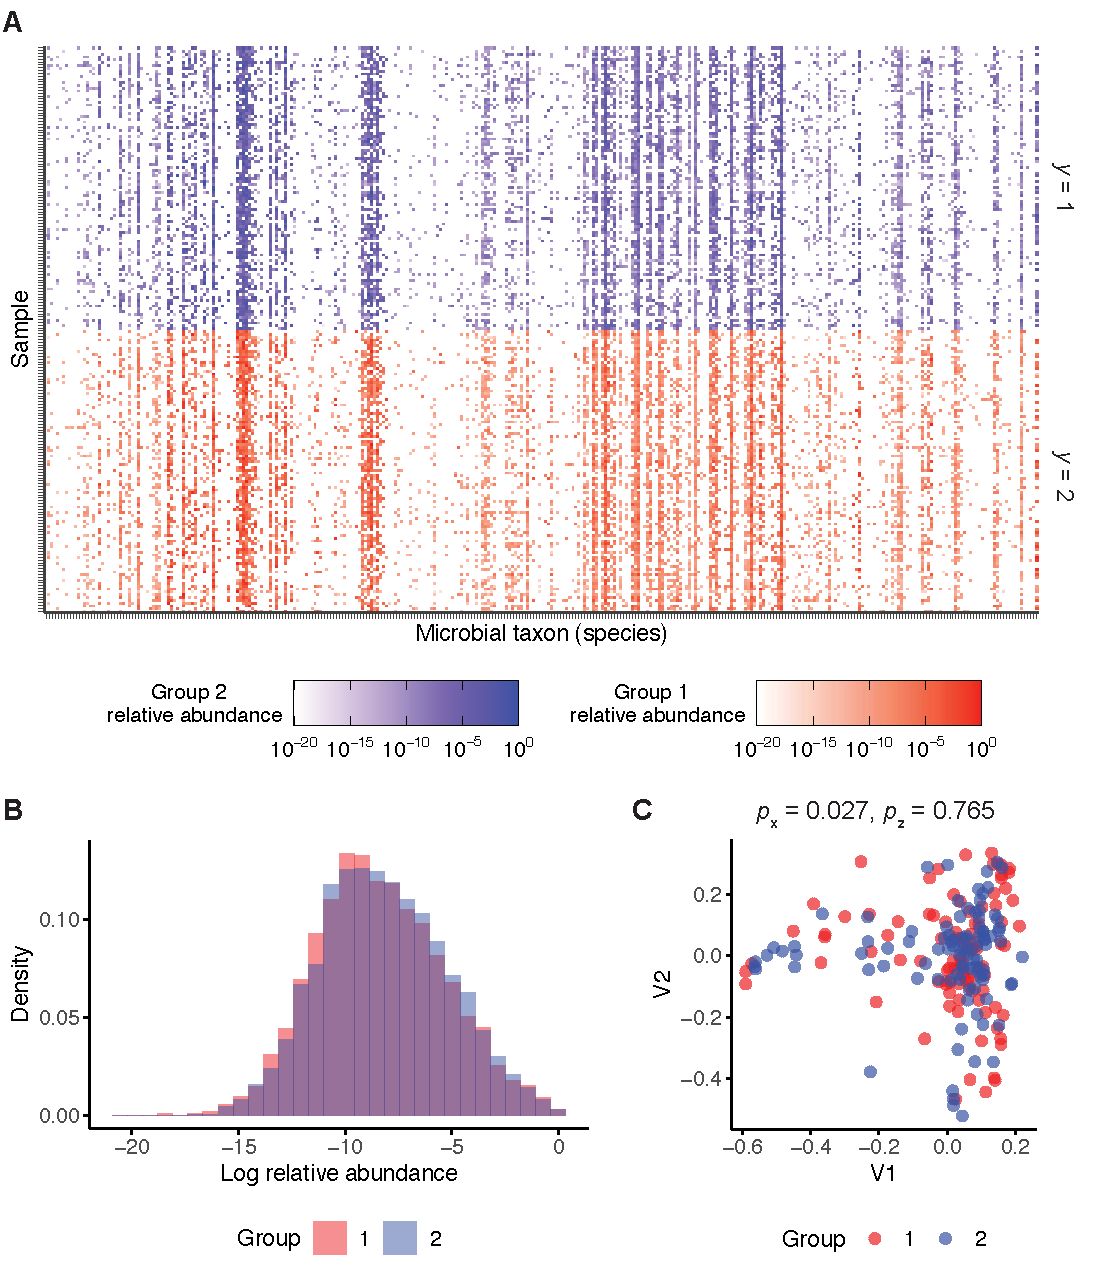
\includegraphics[width=6.5in]{submissions/plos/figures/Fig_S1_rev.pdf}
    \caption[Visualization of a semisynthetic dataset using SparseDOSSA.]{\DIFaddFL{Visualization }\DIFaddendFL of a \DIFdelbeginFL \DIFdelFL{simulated, binary }\DIFdelendFL \DIFaddbeginFL \DIFaddFL{semisynthetic }\DIFaddendFL dataset \DIFdelbeginFL \DIFdelFL{used in this study}\DIFdelendFL \DIFaddbeginFL \DIFaddFL{using SparseDOSSA}\DIFaddendFL . \DIFdelbeginFL \DIFdelFL{Axes }\DIFdelendFL \DIFaddbeginFL \DIFaddFL{(A) Heatmap }\DIFaddendFL of \DIFdelbeginFL \DIFdelFL{each plot correspond to orthonormal vectors that were obtained through eigendecomposition }\DIFdelendFL \DIFaddbeginFL \DIFaddFL{its log-scaled relative abundance by its microbial taxa and sample number. (B) Density histogram }\DIFaddendFL of the \DIFdelbeginFL \DIFdelFL{design matrix $\mathbf{X}$. Alignment on the axis v1 indicates that the samples have been normalized }\DIFdelendFL \DIFaddbeginFL \DIFaddFL{data and }\DIFaddendFL (\DIFdelbeginFL \DIFdelFL{Eq 9, main text}\DIFdelendFL \DIFaddbeginFL \DIFaddFL{C}\DIFaddendFL ) \DIFdelbeginFL \DIFdelFL{. Denoted }\DIFdelendFL \DIFaddbeginFL \DIFaddFL{principal coordinates analysis (PCoA) and PERMANOVA $p$-values based on PCoA results }\DIFaddendFL with \DIFdelbeginFL \DIFdelFL{different colors }\DIFdelendFL \DIFaddbeginFL \DIFaddFL{Euclidean distance ($p_\mathbf{z}$) }\DIFaddendFL and \DIFdelbeginFL \DIFdelFL{shapes are two groups that follow truncated normal distributions }\DIFdelendFL \DIFaddbeginFL \DIFaddFL{original structure }\DIFaddendFL with \DIFdelbeginFL \DIFdelFL{different means but the same covariance }\DIFdelendFL \DIFaddbeginFL \DIFaddFL{Bray-Curtis dissimilarity }\DIFaddendFL (\DIFdelbeginFL \DIFdelFL{Eq 8,main text.}\DIFdelendFL \DIFaddbeginFL \DIFaddFL{$p_\mathbf{x}$}\DIFaddendFL )\DIFaddbeginFL \DIFaddFL{. $N=200$ samples were generated as described.}\DIFaddendFL }
    \DIFdelbeginFL %DIFDELCMD < \label{fig:sim_data_2d}
%DIFDELCMD < %%%
\DIFdelendFL \DIFaddbeginFL \label{fig:sim_data_vis}
\DIFaddendFL \end{figure}
\clearpage

\DIFaddbegin \begin{figure}[h!]
    \centering
    \includegraphics[width=6.5in]{submissions/plos/figures/Fig_S2_rev.pdf}
    \caption[PERMANOVA $p$-values from $F$-informed MDS representations using semisynthetic data.]{\DIFaddFL{PERMANOVA $p$-values from $F$-informed MDS representations using semisynthetic data. $p$-values were plotted against the number of $F$-MDS training epochs for every hyperparameter $\lambda$. Triplicate datasets with size $N=50,100,200,500$ were evaluated. Once $p_\mathbf{z}$ reached to 1 during iteration, the majorization operation was discontinued (e.g., replicate 3 with $N=50$, $\lambda = 0.04$).}}
    \label{fig:sim_fmds_track}
\end{figure}
\clearpage

\DIFaddend \begin{figure}
    \centering
    \DIFdelbeginFL %DIFDELCMD < \includegraphics[width=5in]{submissions/plos/figures/Fig_S2.pdf}
%DIFDELCMD <     \caption[Shepard plot from 4D simulated dataset with seven ordination methods.]{%%%
\DIFdelFL{Shepard plot of simulated dataset (first replicate) }\DIFdelendFL \DIFaddbeginFL \includegraphics[width=6.5in]{submissions/plos/figures/Fig_S3_rev.pdf}
    \caption[Pairwise distance analyses from $F$-informed MDS and supervised MDS.]{\DIFaddFL{Pairwise distance analyses from $F$-informed MDS and supervised MDS }\DIFaddendFL using \DIFdelbeginFL \DIFdelFL{seven dimension reduction methods}\DIFdelendFL \DIFaddbeginFL \DIFaddFL{semisynthetic data}\DIFaddendFL . The plots are titled with the \DIFdelbeginFL \DIFdelFL{respective method }\DIFdelendFL \DIFaddbeginFL \DIFaddFL{dataset size $N$ }\DIFaddendFL and \DIFaddbeginFL \DIFaddFL{compared across different methods with }\DIFaddendFL hyperparameter values as follows: $\lambda$, $F$-MDS; $\alpha$, superMDS\DIFdelbeginFL \DIFdelFL{; Nearest neighbors number, supervised }\DIFdelendFL \DIFaddbeginFL \DIFaddFL{. After calculating pairwise distances with Bray-Curtis dissimilarity }\DIFaddendFL (\DIFdelbeginFL \DIFdelFL{-S}\DIFdelendFL \DIFaddbeginFL \DIFaddFL{original}\DIFaddendFL ) \DIFdelbeginFL \DIFdelFL{or unsupervised }\DIFdelendFL \DIFaddbeginFL \DIFaddFL{and Euclidean }\DIFaddendFL (\DIFdelbeginFL \DIFdelFL{-U}\DIFdelendFL \DIFaddbeginFL \DIFaddFL{2D representation}\DIFaddendFL )\DIFdelbeginFL \DIFdelFL{UMAP; Perplexity}\DIFdelendFL , \DIFdelbeginFL \DIFdelFL{t-SNE; Shortest dissimilarities number, Isomap. X- }\DIFdelendFL \DIFaddbeginFL \DIFaddFL{(B) their Pearson correlation coefficient }\DIFaddendFL and \DIFdelbeginFL \DIFdelFL{Y-axis denote the pairwise distance in the original and embedding dimensions, respectively}\DIFdelendFL \DIFaddbeginFL \DIFaddFL{(C) normalized stress (Stress-1) were obtained}\DIFaddendFL . \DIFaddbeginFL \DIFaddFL{Error bars are standard deviation of triplicates.}\DIFaddendFL }
    \DIFdelbeginFL %DIFDELCMD < \label{fig:shepard_sim_all}
%DIFDELCMD < %%%
\DIFdelendFL \DIFaddbeginFL \label{fig:sim_fmds_smds}
\DIFaddendFL \end{figure}
\clearpage

\begin{figure}
    \centering
    \DIFdelbeginFL %DIFDELCMD < \includegraphics[width=5in]{submissions/plos/figures/Fig_S3.pdf}
%DIFDELCMD <     \caption[\textit{F}-correlation plot from simulated dataset.]{%%%
\textit{\DIFdelFL{F}}%DIFAUXCMD
\DIFdelFL{-correlation plot with simulated data. Pseudo }\DIFdelendFL \DIFaddbeginFL \includegraphics[width=6.5in]{submissions/plos/figures/Fig_S4_rev_gridsearch.pdf}
    \caption[Hyperparameter selection using grid search.]{\DIFaddFL{Hyperparameter selection for }\DIFaddendFL $F$\DIFdelbeginFL \DIFdelFL{-ratios were calculated in }\DIFdelendFL \DIFaddbeginFL \DIFaddFL{-informed MDS using grid search. An objective function $f_{\rm obj}(\lambda)$ was defined to simultaneously reflect }\DIFaddendFL the \DIFaddbeginFL \DIFaddFL{number of training epochs and the preservation of the }\DIFaddendFL original \DIFdelbeginFL \DIFdelFL{dimension }\DIFdelendFL \DIFaddbeginFL \DIFaddFL{structure }\DIFaddendFL (\DIFdelbeginFL \DIFdelFL{x-axis}\DIFdelendFL \DIFaddbeginFL \DIFaddFL{see Equation \ref{eq:def_grid_search}}\DIFaddendFL )\DIFdelbeginFL \DIFdelFL{and in each dimension reduction method }\DIFdelendFL \DIFaddbeginFL \DIFaddFL{. }\DIFaddendFL (\DIFdelbeginFL \DIFdelFL{y-axis}\DIFdelendFL \DIFaddbeginFL \DIFaddFL{A}\DIFaddendFL ) \DIFdelbeginFL \DIFdelFL{using first replicate of the simulated }\DIFdelendFL \DIFaddbeginFL \DIFaddFL{For each semisynthetic }\DIFaddendFL dataset \DIFdelbeginFL \DIFdelFL{. Pseudo $F$'s were calculated by randomly permuting labels by 500 times. Highlighted with red denotes }\DIFdelendFL \DIFaddbeginFL \DIFaddFL{size $N$, $f_{\rm obj}(\lambda)$ is plotted against }\DIFaddendFL the \DIFdelbeginFL \DIFdelFL{location }\DIFdelendFL \DIFaddbeginFL \DIFaddFL{hyperparameter $\lambda$. The minimum value }\DIFaddendFL of \DIFdelbeginFL \DIFdelFL{$F$'s from unpermuted labels}\DIFdelendFL \DIFaddbeginFL \DIFaddFL{$f_{\rm obj}(\lambda)$ is highlighted in red}\DIFaddendFL . \DIFdelbeginFL \DIFdelFL{Each plot }\DIFdelendFL \DIFaddbeginFL \DIFaddFL{(B) The optimal hyperparameter $\lambda_{\rm min}$ }\DIFaddendFL is \DIFdelbeginFL \DIFdelFL{titled }\DIFdelendFL \DIFaddbeginFL \DIFaddFL{plotted against dataset size $N$, }\DIFaddendFL with \DIFdelbeginFL \DIFdelFL{the method and hyperparameter used}\DIFdelendFL \DIFaddbeginFL \DIFaddFL{each dataset represented by a symbol}\DIFaddendFL .}
    \DIFdelbeginFL %DIFDELCMD < \label{fig:f_corr_sim_all}
%DIFDELCMD < %%%
\DIFdelendFL \DIFaddbeginFL \label{fig:fmds_gridsearch}
\DIFaddendFL \end{figure}
\clearpage

\begin{figure}
    \centering
    \DIFdelbeginFL %DIFDELCMD < \includegraphics[width=5in]{submissions/plos/figures/Fig_S4.pdf}
%DIFDELCMD <     %%%
%DIFDELCMD < \caption[Shepard plot from algal microbiome dataset with eight ordination methods.]{%
{%DIFAUXCMD
\DIFdelFL{Shepard plot of algal-associated bacterial community data using eight dimension reduction methods. The plots are titled with the respective method and hyperparameter values as follows: $\lambda$, $F$-MDS; $\alpha$, superMDS; Nearest neighbors number, supervised (-S) or unsupervised (-U) UMAP; Perplexity, t-SNE; Shortest dissimilarities number, Isomap; none, neural network (NN). X- and Y-axis denote distances in the original and embedding dimensions, respectively.}}
    %DIFAUXCMD
%DIFDELCMD < \label{fig:shepard_alga_all}
%DIFDELCMD < %%%
\DIFdelendFL \DIFaddbeginFL \includegraphics[width=5.05in]{submissions/plos/figures/Fig_S5_rev.pdf}
    \caption[Comparison of quality metrics of benchmark ordination methods.]{\DIFaddFL{Comparison of quality metrics of ordination methods evaluated on semisynthetic datasets. Trustworthiness and continuity to evaluate (A) Local structural preservation is assessed using trustworthiness and continuity. (B) Global structural preservation is similarly evaluated with trustworthiness and continuity. (C) Global distortion is quantified by Stress-1 and Pearson correlation of Shepard diagrams. (D) Preservation of statistical inference is measured by the $F$-rank-ratio and $F$-correlation using randomly permuted label sets. The following hyperparameters were used for each method: $\lambda$ for $F$-MDS, number of neighbors $n$ for UMAP (both supervised (-S) and unsupervised (-U)), perplexity (perp) for t-SNE, and the number of shortest dissimilarities $n$ for Isomap. Error bars represent the standard deviation across triplicate measurements.}}
    \label{fig:sim_eval_all}
\DIFaddendFL \end{figure}
\clearpage

\begin{figure}
    \centering
    \DIFdelbeginFL %DIFDELCMD < \includegraphics[width=5in]{submissions/plos/figures/Fig_S5.pdf}
%DIFDELCMD <     %%%
%DIFDELCMD < \caption[\textit{F}-correlation plot from algal microbiome dataset.]{%
{%DIFAUXCMD
\textit{\DIFdelFL{F}}%DIFAUXCMD
\DIFdelFL{-correlation plot from algal microbiome dataset. Pseudo $F$-ratios comparing the original dimension (x-axis) and from eight dimension reduction methods (y-axis) with algal microbiome data. Pseudo $F$'s were calculated by randomly permuting labels by 500 times. Highlighted with red denotes the location of $F$'s from unpermuted labels. Each plot is titled with the method and hyperparameter used.}}
    %DIFAUXCMD
%DIFDELCMD < \label{fig:f_corr_alga_all}
%DIFDELCMD < %%%
\DIFdelendFL \DIFaddbeginFL \includegraphics[width=5in]{submissions/plos/figures/Fig_S6_rev.pdf}
    \caption[Shepard plot from algal microbiome dataset with eight ordination methods.]{\DIFaddFL{Shepard plot of algal-associated bacterial community data using eight dimension reduction methods. The plots are titled with the respective method and hyperparameter values as follows: $\lambda$, $F$-MDS; $\alpha$, superMDS; Nearest neighbors number, supervised (-S) or unsupervised (-U) UMAP; Perplexity, t-SNE; Shortest dissimilarities number, Isomap; none, neural network (NN). X- and Y-axis denote distances in the original and embedding dimensions, respectively.}}
    \label{fig:shepard_alga_all}
\DIFaddendFL \end{figure}
\clearpage

\begin{figure}
    \centering
    \DIFdelbeginFL %DIFDELCMD < \includegraphics[width=6.5in]{submissions/plos/figures/Fig_S6.pdf}
%DIFDELCMD <     \caption[Pairs plot of simulated, trinary data.]{%%%
\DIFdelFL{Pairs plot of trinary, four-dimensional simulated data. Each row and column corresponds to respective axis for the projection. Denoted with different colors or shapes are the trinary groups that follow normal distributions with different means but the same covariance (Eq 10, main text.) }%DIFDELCMD < \MBLOCKRIGHTBRACE
%DIFDELCMD <     \label{fig:sim_data_4d}
%DIFDELCMD < %%%
\DIFdelendFL \DIFaddbeginFL \includegraphics[width=5in]{submissions/plos/figures/Fig_S7_rev.pdf}
    \caption[\textit{F}-correlation plot from algal microbiome dataset.]{\textit{\DIFaddFL{F}}\DIFaddFL{-correlation plot from algal microbiome dataset. Pseudo $F$-ratios comparing the original dimension (x-axis) and from eight dimension reduction methods (y-axis) with algal microbiome data. Pseudo $F$'s were calculated by randomly permuting labels by 500 times. Highlighted with red denotes the location of $F$'s from unpermuted labels. Each plot is titled with the method and hyperparameter used.}}
    \label{fig:f_corr_alga_all}
\DIFaddendFL \end{figure}
\clearpage

\begin{figure}
    \centering
    \DIFdelbeginFL %DIFDELCMD < \includegraphics[width=6.5in]{submissions/plos/figures/Fig_S7.pdf}
%DIFDELCMD <     %%%
\DIFdelendFL \DIFaddbeginFL \includegraphics[width=6.5in]{submissions/plos/figures/Fig_S8_rev.pdf}
    \DIFaddendFL \caption[Cluster centroid and variances of $F$-MDS representations.]{Cluster \DIFdelbeginFL \DIFdelFL{centroid }\DIFdelendFL \DIFaddbeginFL \DIFaddFL{centroids }\DIFaddendFL and variances of $F$-MDS representations \DIFaddbeginFL \DIFaddFL{are shown }\DIFaddendFL for \DIFdelbeginFL \DIFdelFL{simulated dataset }\DIFdelendFL \DIFaddbeginFL \DIFaddFL{semisynthetic datasets of size $N=50$ }\DIFaddendFL (\DIFdelbeginFL \DIFdelFL{A-C}\DIFdelendFL \DIFaddbeginFL \DIFaddFL{A–C}\DIFaddendFL )\DIFaddbeginFL \DIFaddFL{, $N=100$ (D–F), $N=200$ (G–I), $N=500$ (J–L) }\DIFaddendFL and \DIFaddbeginFL \DIFaddFL{for the }\DIFaddendFL algal microbiome (\DIFdelbeginFL \DIFdelFL{D-F}\DIFdelendFL \DIFaddbeginFL \DIFaddFL{M–O}\DIFaddendFL ). \DIFdelbeginFL \DIFdelFL{A,D: Distance }\DIFdelendFL \DIFaddbeginFL \DIFaddFL{The first column in each row displays the distance }\DIFaddendFL between group centroids. \DIFdelbeginFL \DIFdelFL{B,E: Variance }\DIFdelendFL \DIFaddbeginFL \DIFaddFL{The second and third columns show the variance }\DIFaddendFL of each group\DIFdelbeginFL \DIFdelFL{measured in its long-axis. C}\DIFdelendFL , \DIFdelbeginFL \DIFdelFL{F: Variance of each group }\DIFdelendFL measured \DIFdelbeginFL \DIFdelFL{in its short-axis}\DIFdelendFL \DIFaddbeginFL \DIFaddFL{along the long and short principal axes, respectively}\DIFaddendFL . For \DIFdelbeginFL \DIFdelFL{simulated dataset error bars denote standard deviation of triplicates. For }\DIFdelendFL \DIFaddbeginFL \DIFaddFL{the }\DIFaddendFL variance \DIFdelbeginFL \DIFdelFL{calculations}\DIFdelendFL \DIFaddbeginFL \DIFaddFL{panels}\DIFaddendFL , blue and red colors denote \DIFdelbeginFL \DIFdelFL{group }\DIFdelendFL \DIFaddbeginFL \DIFaddFL{groups }\DIFaddendFL 1 and \DIFdelbeginFL \DIFdelFL{2, respectively}\DIFdelendFL \DIFaddbeginFL \DIFaddFL{2. Error bars represent the standard deviation across triplicate measurements}\DIFaddendFL .}
    \label{fig:fmds_rep_analysis}
\end{figure}
\clearpage

%DIF <  \begin{figure}
%DIF <      \centering
%DIF <      \includegraphics[width=6.5in]{submissions/nips/figures/site-config-all.pdf}
%DIF <      \caption[Visualization of bacterial community using FMDS.]{Visualization of bacterial community using proposed FMDS. Microbial community samples are collected from Site 1 (top row) and Site 2 (bottom row).}
%DIF <      \label{fig:site_config_all}
%DIF <  \end{figure}
%DIF <  \clearpage
\DIFdelbegin %DIFDELCMD < 

%DIFDELCMD < %%%
%DIF <  \begin{figure}
%DIF <      \centering
%DIF <      \includegraphics[width=6.5in]{submissions/nips/figures/shepard_site.png}
%DIF <      \caption[Shepard plot of community dataset.]{Shepard plot in microbial community data collected from site 1 (first row) and site 2 (second row) for a range of hyperparameters.}
%DIF <      \label{fig:shepard_site}
%DIF <  \end{figure}
%DIF <  \clearpage
%DIFDELCMD < 

%DIFDELCMD < %%%
%DIF <  \begin{figure}
%DIF <      \centering
%DIF <      \includegraphics[width=6.5in]{submissions/ISMB/figures/cirrhosis.pdf}
%DIF <      \caption[Visualization of cirrhosis patients and healthy human gut microbiome.]{Visualization of cirrhosis patients and healthy human gut microbiome. The following hyperparameters were used: $\lambda=0.3$ (FMDS), neighbors $=10$ (UMAP-S), neighbors $=30$ (UMAP-U), perplexity$=7$ (t-SNE), $K=10$ (Isomap).}
%DIF <      \label{fig:cirr}
%DIF <  \end{figure}
%DIF <  \clearpage
\DIFdelend \DIFaddbegin \begin{figure}
    \centering
    \includegraphics[width=6.5in]{submissions/plos/figures/Fig_S9_rev.pdf}
    \caption[Visualization of a semisynthetic ternary dataset.]{\DIFaddFL{Visualization of a semisynthetic ternary dataset. (A) Heatmap of its log-scaled relative abundance by its microbial taxa and sample number. (B) Density histogram of the data and (C) principal coordinates analysis (PCoA) and PERMANOVA $p$-values based on PCoA results with Euclidean distance ($p_\mathbf{z}$) and original structure with Bray-Curtis dissimilarity ($p_\mathbf{x}$). $N=75$ semisynthetic data were generated.}}
    \label{fig:sim_ternary_vis}
\end{figure}
\clearpage
\DIFaddend 


\begin{singlespace}
\bibliographystyle{acm}
\documentclass[11pt]{article}
%DIF LATEXDIFF DIFFERENCE FILE


%%%%%%%%%%%%%%%%%%%%%%%%%%%%%%%%%%%%%%%%%%%%%%%%%%%%%%%%%
%%%%%%%%%%%%%%%%%%%%%%%%% Setup %%%%%%%%%%%%%%%%%%%%%%%%%
\usepackage[margin=1in]{geometry}
\usepackage{fmtcount} % 1st, 2nd...
\usepackage[english]{babel}
\usepackage{soul} % spacing
\usepackage{enumerate} % change enum label
\usepackage{framed} % frame pagebreak
\usepackage{authblk}
\usepackage{setspace}
\usepackage{tocloft}

%%%%% Math, Code 
\usepackage{amsmath}
\usepackage{amsfonts}
\usepackage{amssymb}
\usepackage{amsthm}
\usepackage{amscd}
\usepackage{array}
\usepackage{mathtools} 
\usepackage{verbatim}
\usepackage{fancyvrb} % verbatim
\usepackage{algpseudocode}
\usepackage{algorithm}

%%%%% Graphic, Figure, Table
\usepackage{graphicx}
\usepackage{epstopdf}
\usepackage{xcolor}
\usepackage[labelsep=none]{caption}
\usepackage{subcaption}
\usepackage{multirow} % table
\usepackage{longtable} % table to next page
\usepackage{rotating}
\usepackage{wrapfig} % wrap fig, tbl with text

%%%%% Bib, Cite
\usepackage{url}
\usepackage{cite}
\usepackage{fancyref}
\usepackage{hyperref}
\hypersetup{linktocpage}

%%%%%% Setup
% \captionsetup{compatibility=false} %subfig
% \DeclareCaptionLabelFormat{Sformat}{S#2 #1}
% \captionsetup[figure]{labelformat=Sformat}
% \captionsetup[table]{labelformat=Sformat}
\hypersetup{colorlinks=false}
\setlength{\parskip}{0.5em}

\newtheorem{thm}{Theorem}[section]
\newtheorem{cor}[thm]{Corollary}
\newtheorem{lem}[thm]{Lemma}
\newtheorem{prop}[thm]{Proposition}
\newtheorem{dfn}{Definition}
\newtheorem{ex}{Example}
\newtheorem{cmt}{Cmt}[section]
\newtheorem{rmk}{Remark}[section]
\newcommand{\rb}[1]{\raisebox{-.5em}[0pt]{#1}}
\newcommand{\1}{{\rm 1}\kern-0.24em{\rm I}}
\newcommand{\cN}{\mathcal{N}}
\newcommand{\cO}{\mathcal{O}}
\renewcommand{\mid}{\, | \ , }
\makeatletter
\renewcommand\theequation{S\@arabic\c@equation}
\makeatother

\renewcommand\Affilfont{\normalsize}
% \renewcommand{\baselinestretch}{1.3}

\DeclareMathOperator*{\argmin}{arg\,min}
\DeclareMathOperator*{\argmax}{arg\,max}
\DeclareMathOperator*{\bbr}{\mathbb{R}}
%%%%%%%%%%%%%%%%%%%%%%%%%%%%%%%%%%%%%%%%%%%%%%%%%%%%%%%
%%%%%%%%%%%%%%%%%%%%%%%%%%%%%%%%%%%%%%%%%%%%%%%%%%%%%%%

\title{Supporting Information of ``Multidimensional scaling informed by $F$-statistic: Visualizing grouped microbiome data with inference''}
\author[1\dag]{Hyungseok Kim}
\author[2\dag]{Soobin Kim}
\author[3]{Jeffrey A. Kimbrel}
\author[3]{Megan M. Morris}
\author[3]{Xavier Mayali}
\author[1$*$]{Cullen R. Buie}
\affil[1]{Massachusetts Institute of Technology, Cambridge, MA, USA}
\affil[2]{University of California, Davis, Davis, CA, USA}
\affil[3]{Lawrence Livermore National Laboratory, Livermore, CA, USA}
\affil[$\dagger$] {These authors contributed equally to this work.}
\affil[$^*$]{Correspondence: crb@mit.edu.}
% \author{}
\date{}
%DIF PREAMBLE EXTENSION ADDED BY LATEXDIFF
%DIF UNDERLINE PREAMBLE %DIF PREAMBLE
\RequirePackage[normalem]{ulem} %DIF PREAMBLE
\RequirePackage{color}\definecolor{RED}{rgb}{1,0,0}\definecolor{BLUE}{rgb}{0,0,1} %DIF PREAMBLE
\providecommand{\DIFaddtex}[1]{{\protect\color{blue}\uwave{#1}}} %DIF PREAMBLE
\providecommand{\DIFdeltex}[1]{{\protect\color{red}\sout{#1}}}                      %DIF PREAMBLE
%DIF SAFE PREAMBLE %DIF PREAMBLE
\providecommand{\DIFaddbegin}{} %DIF PREAMBLE
\providecommand{\DIFaddend}{} %DIF PREAMBLE
\providecommand{\DIFdelbegin}{} %DIF PREAMBLE
\providecommand{\DIFdelend}{} %DIF PREAMBLE
\providecommand{\DIFmodbegin}{} %DIF PREAMBLE
\providecommand{\DIFmodend}{} %DIF PREAMBLE
%DIF FLOATSAFE PREAMBLE %DIF PREAMBLE
\providecommand{\DIFaddFL}[1]{\DIFadd{#1}} %DIF PREAMBLE
\providecommand{\DIFdelFL}[1]{\DIFdel{#1}} %DIF PREAMBLE
\providecommand{\DIFaddbeginFL}{} %DIF PREAMBLE
\providecommand{\DIFaddendFL}{} %DIF PREAMBLE
\providecommand{\DIFdelbeginFL}{} %DIF PREAMBLE
\providecommand{\DIFdelendFL}{} %DIF PREAMBLE
%DIF HYPERREF PREAMBLE %DIF PREAMBLE
\providecommand{\DIFadd}[1]{\texorpdfstring{\DIFaddtex{#1}}{#1}} %DIF PREAMBLE
\providecommand{\DIFdel}[1]{\texorpdfstring{\DIFdeltex{#1}}{}} %DIF PREAMBLE
\newcommand{\DIFscaledelfig}{0.5}
%DIF HIGHLIGHTGRAPHICS PREAMBLE %DIF PREAMBLE
\RequirePackage{settobox} %DIF PREAMBLE
\RequirePackage{letltxmacro} %DIF PREAMBLE
\newsavebox{\DIFdelgraphicsbox} %DIF PREAMBLE
\newlength{\DIFdelgraphicswidth} %DIF PREAMBLE
\newlength{\DIFdelgraphicsheight} %DIF PREAMBLE
% store original definition of \includegraphics %DIF PREAMBLE
\LetLtxMacro{\DIFOincludegraphics}{\includegraphics} %DIF PREAMBLE
\newcommand{\DIFaddincludegraphics}[2][]{{\color{blue}\fbox{\DIFOincludegraphics[#1]{#2}}}} %DIF PREAMBLE
\newcommand{\DIFdelincludegraphics}[2][]{% %DIF PREAMBLE
\sbox{\DIFdelgraphicsbox}{\DIFOincludegraphics[#1]{#2}}% %DIF PREAMBLE
\settoboxwidth{\DIFdelgraphicswidth}{\DIFdelgraphicsbox} %DIF PREAMBLE
\settoboxtotalheight{\DIFdelgraphicsheight}{\DIFdelgraphicsbox} %DIF PREAMBLE
\scalebox{\DIFscaledelfig}{% %DIF PREAMBLE
\parbox[b]{\DIFdelgraphicswidth}{\usebox{\DIFdelgraphicsbox}\\[-\baselineskip] \rule{\DIFdelgraphicswidth}{0em}}\llap{\resizebox{\DIFdelgraphicswidth}{\DIFdelgraphicsheight}{% %DIF PREAMBLE
\setlength{\unitlength}{\DIFdelgraphicswidth}% %DIF PREAMBLE
\begin{picture}(1,1)% %DIF PREAMBLE
\thicklines\linethickness{2pt} %DIF PREAMBLE
{\color[rgb]{1,0,0}\put(0,0){\framebox(1,1){}}}% %DIF PREAMBLE
{\color[rgb]{1,0,0}\put(0,0){\line( 1,1){1}}}% %DIF PREAMBLE
{\color[rgb]{1,0,0}\put(0,1){\line(1,-1){1}}}% %DIF PREAMBLE
\end{picture}% %DIF PREAMBLE
}\hspace*{3pt}}} %DIF PREAMBLE
} %DIF PREAMBLE
\LetLtxMacro{\DIFOaddbegin}{\DIFaddbegin} %DIF PREAMBLE
\LetLtxMacro{\DIFOaddend}{\DIFaddend} %DIF PREAMBLE
\LetLtxMacro{\DIFOdelbegin}{\DIFdelbegin} %DIF PREAMBLE
\LetLtxMacro{\DIFOdelend}{\DIFdelend} %DIF PREAMBLE
\DeclareRobustCommand{\DIFaddbegin}{\DIFOaddbegin \let\includegraphics\DIFaddincludegraphics} %DIF PREAMBLE
\DeclareRobustCommand{\DIFaddend}{\DIFOaddend \let\includegraphics\DIFOincludegraphics} %DIF PREAMBLE
\DeclareRobustCommand{\DIFdelbegin}{\DIFOdelbegin \let\includegraphics\DIFdelincludegraphics} %DIF PREAMBLE
\DeclareRobustCommand{\DIFdelend}{\DIFOaddend \let\includegraphics\DIFOincludegraphics} %DIF PREAMBLE
\LetLtxMacro{\DIFOaddbeginFL}{\DIFaddbeginFL} %DIF PREAMBLE
\LetLtxMacro{\DIFOaddendFL}{\DIFaddendFL} %DIF PREAMBLE
\LetLtxMacro{\DIFOdelbeginFL}{\DIFdelbeginFL} %DIF PREAMBLE
\LetLtxMacro{\DIFOdelendFL}{\DIFdelendFL} %DIF PREAMBLE
\DeclareRobustCommand{\DIFaddbeginFL}{\DIFOaddbeginFL \let\includegraphics\DIFaddincludegraphics} %DIF PREAMBLE
\DeclareRobustCommand{\DIFaddendFL}{\DIFOaddendFL \let\includegraphics\DIFOincludegraphics} %DIF PREAMBLE
\DeclareRobustCommand{\DIFdelbeginFL}{\DIFOdelbeginFL \let\includegraphics\DIFdelincludegraphics} %DIF PREAMBLE
\DeclareRobustCommand{\DIFdelendFL}{\DIFOaddendFL \let\includegraphics\DIFOincludegraphics} %DIF PREAMBLE
%DIF END PREAMBLE EXTENSION ADDED BY LATEXDIFF

\begin{document}

\renewcommand*\contentsname{\normalsize List of Supplementary Notes}
\makeatletter
\renewcommand{\tableofcontents}{\@starttoc{toc}}
\renewcommand*\l@section{\@dottedtocline{1}{0em}{6.3em}}
\let\l@table\l@content
\makeatother

\makeatletter
\renewcommand{\listoffigures}{\@starttoc{lof}}
\renewcommand*\l@figure{\@dottedtocline{1}{0em}{3.5em}}
\let\l@table\l@figure
\makeatother

\makeatletter
\renewcommand{\listoftables}{\@starttoc{lot}}
\renewcommand*\l@table{\@dottedtocline{1}{0em}{4.5em}}
\let\l@table\l@table
\makeatother

\renewcommand\thesection{S\arabic{section} Appendix.}
\makeatletter
\renewcommand*{\@seccntformat}[1]{\csname the#1\endcsname\hspace{0.5em}}
\makeatother

\renewcommand{\figurename}{\!\!}
\let\standardthefigure\thefigure
\renewcommand\thefigure{S\standardthefigure\ Fig.\ }
\addtolength{\cftfignumwidth}{15pt}

\renewcommand{\tablename}{\!\!}
\let\standardthetable\thetable
\renewcommand\thetable{S\standardthetable\ Table.\ }

% \renewcommand{\algorithmname}{\!\!}
\let\standardthealgorithm\thealgorithm
\renewcommand\thealgorithm{S\standardthealgorithm}

\maketitle
% \def\thefootnote{\arabic{footnote}}

{\noindent\normalsize\bf List of Supplementary Information}
\tableofcontents
\listoffigures
\listoftables
\clearpage


\section{\DIFdelbegin \DIFdel{Mapping }\DIFdelend \DIFaddbegin \DIFadd{Objective }\DIFaddend function for \DIFaddbegin \DIFadd{computing }\DIFaddend $F$-MDS\DIFdelbegin \DIFdel{.}\DIFdelend } \label{sec:app1}

\DIFdelbegin \DIFdel{In this section, we explain a procedure of deriving a }\DIFdelend \DIFaddbegin \DIFadd{First, we derive a }\DIFaddend mapping function $f_\mathbf{z}(F_\mathbf{x})$ \DIFdelbegin \DIFdel{that is used to minimize }\DIFdelend \DIFaddbegin \DIFadd{for minimizing }\DIFaddend an objective function \DIFdelbegin \DIFdel{for }\DIFdelend \DIFaddbegin \DIFadd{and }\DIFaddend computing $F$-informed MDS.
The \DIFdelbegin \DIFdel{confirmatory term of the objective function (Eq 5 of the main text) is specifically designed }\DIFdelend \DIFaddbegin \DIFadd{mapping function guides }\DIFaddend to minimize a difference in $p$-values testing \DIFdelbegin \DIFdel{for group difference by representations }\DIFdelend \DIFaddbegin \DIFadd{group differences }\DIFaddend under the original $S$- and \DIFdelbegin \DIFdel{two-dimensions}\DIFdelend \DIFaddbegin \DIFadd{two-dimensional embedding through the confirmatory term of the objective (see Eq 5 of the main text)}\DIFaddend .
These \textit{p}-values are obtained from an empirical distribution of the pseudo-$F$s by permuted labels \cite{anderson01} \DIFdelbegin \DIFdel{. 
In other words, by denoting a label set as $[y_i]$ ($i=1,\cdots N$) and its permuted set as $[y_i^\pi]$ with operator $\pi$, we express each }\DIFdelend \DIFaddbegin \DIFadd{(Eq 4, main text). 
For a given label set $[y_i]_{i=1}^{N}$ and its group number $G$, a permuted label set $[y_i^\Pi]_{i=1}^{N}$ and }\DIFaddend $F$\DIFdelbegin \DIFdel{-statistic as
}\DIFdelend \DIFaddbegin \DIFadd{-statistics are expressed as
}\DIFaddend \begin{equation}
\DIFdelbegin %DIFDELCMD < \begin{aligned}
%DIFDELCMD < F^\pi_\mathbf{x} &= 
%DIFDELCMD < \left(\frac{\sum_{i,j}d_{ij}^2}{2\sum_{i,j}d_{ij}^2\,\1\{y_i^\pi = y_j^\pi\}} -1 \right) \cdot (N-2), \\
%DIFDELCMD < F^\pi_\mathbf{z} &= 
%DIFDELCMD < \left(\frac{\sum_{i,j}\|\mathbf{z}_i - \mathbf{z}_j\|_2^2}{2\sum_{i,j}\|\mathbf{z}_i - \mathbf{z}_j\|_2^2\,\1\{y_i^\pi = y_j^\pi\}} -1 \right) \cdot (N-2).
%DIFDELCMD < \label{eq:map1}
%DIFDELCMD < \end{aligned}%%%
\DIFdelend \DIFaddbegin \begin{aligned}
F^\Pi_\mathbf{x} &= 
\left(\frac{\sum_{i,j}d_{ij}^2}{G \sum_{i,j}d_{ij}^2\,\1\{y_i^\Pi = y_j^\Pi\}} -1 \right) \cdot \frac{N-G}{G-1}, \\
F^\Pi_\mathbf{z} &= 
\left(\frac{\sum_{i,j}\|\mathbf{z}_i - \mathbf{z}_j\|_2^2}{G\sum_{i,j}\|\mathbf{z}_i - \mathbf{z}_j\|_2^2\,\1\{y_i^\Pi = y_j^\Pi\}} -1 \right) \cdot \frac{N-G}{G-1}.
\label{eq:map1}
\end{aligned}\DIFaddend 
\end{equation}
% \end{align} 

It should be noted that the pseudo $F$-ratios can range differently based on how the samples are projected onto 2D. To scale between these two ratios and minimize the difference in $p$-values, we consider a mapping $f_\mathbf{z}: F_\mathbf{x} \rightarrow F_\mathbf{z}$ from a pair of ratios \DIFdelbegin \DIFdel{$(F_\mathbf{x}^{\pi_1}, F_\mathbf{z}^{\pi_2})$ }\DIFdelend \DIFaddbegin \DIFadd{$(F_\mathbf{x}^{\Pi_1}, F_\mathbf{z}^{\Pi_2})$ }\DIFaddend where each element was ordered from two independent sets of repeated permutations. Figure below exemplifies how the $F$-ratios at each dimensionality scaled differently and depended on the choice of hyperparameter $\lambda$. In both settings, the $F$-ratio in $S$-dimension ranged \DIFdelbegin \DIFdel{between zero and six }\DIFdelend \DIFaddbegin \DIFadd{in }[\DIFadd{0,6}] \DIFaddend whereas in 2D representation the ratio ranged in [0,4]. The hyperparameter, however, impacted the detailed relationship between ordered $F_\mathbf{x}$ and ordered $F_\mathbf{x}$, when compared to each other. 

\begin{figure}[h]
    \centering
    \includegraphics[width=5.5in]{submissions/plos/figures/supp-mds_Fval.pdf}
    \caption*{Figure: Mapping pseudo-$F$'s between two dimensionalities. Each $F_\mathbf{x} \text{-} F_\mathbf{z}$ relationship was obtained by permuting labels over 1,000 times, and by setting a hyperparameter $\lambda$ that is used to perform the majorization.}
    \label{fig:mds-fval}
\end{figure}

Using the mapping function $f_\mathbf{z}$, we \DIFdelbegin \DIFdel{now }\DIFdelend derive an exact \DIFdelbegin \DIFdel{form of confirmatory term proposed }\DIFdelend \DIFaddbegin \DIFadd{expression for the confirmatory term introduced }\DIFaddend in the $F$-MDS objective function\DIFdelbegin \DIFdel{(Eq 5 of main text)}\DIFdelend . The proposed form $\left|F_\mathbf{z} - f_\mathbf{z}(F_\mathbf{x})\right|$ measures how \DIFaddbegin \DIFadd{accurately }\DIFaddend the 2D representation \DIFdelbegin \DIFdel{accurately reflected }\DIFdelend \DIFaddbegin \DIFadd{reflects }\DIFaddend the $S$-dimensional distance structure \DIFdelbegin \DIFdel{with respect to }\DIFdelend \DIFaddbegin \DIFadd{regarding }\DIFaddend the sample labels. \DIFdelbegin \DIFdel{Having the }\DIFdelend \DIFaddbegin \DIFadd{A }\DIFaddend difference close to zero indicates that no \DIFdelbegin \DIFdel{additional update with the representation is required (let us denote it as }\DIFdelend \DIFaddbegin \DIFadd{further updates to the representation are required (denoted }\DIFaddend $\mathbf{Z}^*$). \DIFdelbegin \DIFdel{Now by substituting }\DIFdelend \DIFaddbegin \DIFadd{Substituting }\DIFaddend the confirmatory term $\left|F_\mathbf{z} - f_\mathbf{z}(F_\mathbf{x})\right|$ with Equation \ref{eq:map1}, we define \DIFdelbegin \DIFdel{$\1\{y_i^\pi = y_j^\pi\}\coloneqq\epsilon_{ij}$ and write
}\DIFdelend \DIFaddbegin \DIFadd{$\epsilon_{ij}\coloneqq\1\{y_i^\Pi = y_j^\Pi\}$ and write
}\DIFaddend \begin{align}
\mathbf{Z}^* &= \argmin_\mathbf{Z}\,\left|F_\mathbf{z} - f_\mathbf{z}(F_\mathbf{x})\right| \\
& = \argmin_\mathbf{Z}\,\left|\DIFdelbegin \DIFdel{(N-2)}\DIFdelend \DIFaddbegin \DIFadd{\frac{N-G}{G-1}}\DIFaddend \cdot\left(\DIFdelbegin \DIFdel{\frac{\sum_{i,j}\|\mathbf{z}_i - \mathbf{z}_j\|_2^2}{2\sum_{i,j}\epsilon_{ij}\|\mathbf{z}_i - \mathbf{z}_j\|_2^2} }\DIFdelend \DIFaddbegin \DIFadd{\frac{\sum_{i,j}\|\mathbf{z}_i - \mathbf{z}_j\|_2^2}{G\sum_{i,j}\epsilon_{ij}\|\mathbf{z}_i - \mathbf{z}_j\|_2^2} }\DIFaddend -1 \right) - f_\mathbf{z}(F_\mathbf{x})\right| \\
&= \argmin_\mathbf{Z}\,\left|\DIFdelbegin \DIFdel{\frac{\sum_{i,j}\|\mathbf{z}_i - \mathbf{z}_j\|_2^2}{2\sum_{i,j}\epsilon_{ij}\|\mathbf{z}_i - \mathbf{z}_j\|_2^2} }\DIFdelend \DIFaddbegin \DIFadd{\frac{\sum_{i,j}\|\mathbf{z}_i - \mathbf{z}_j\|_2^2}{G\sum_{i,j}\epsilon_{ij}\|\mathbf{z}_i - \mathbf{z}_j\|_2^2} }\DIFaddend -1 - \DIFdelbegin \DIFdel{\frac{f_\mathbf{z}(F_\mathbf{x})}{N-2} }\DIFdelend \DIFaddbegin \DIFadd{\frac{G-1}{N-G}\cdot{f_\mathbf{z}(F_\mathbf{x})} }\DIFaddend \right| \DIFdelbegin %DIFDELCMD < \\
%DIFDELCMD < &%%%
\DIFdel{= \argmin_\mathbf{Z}\,}%DIFDELCMD < \left| %%%
\DIFdel{\frac{\sum_{i,j}\|\mathbf{z}_i - \mathbf{z}_j\|_2^2 - 2\sum_{i,j}\epsilon_{ij}\|\mathbf{z}_i - \mathbf{z}_j\|_2^2 \cdot [1+f_\mathbf{z}(F_\mathbf{x})/(N-2)]}{2\sum_{i,j}\epsilon_{ij}\|\mathbf{z}_i - \mathbf{z}_j\|_2^2} }%DIFDELCMD < \right| %%%
\DIFdelend \label{eq:pre_approx}\\
&\approx \argmin_\mathbf{Z}\,\left| \sum_{i,j}\|\mathbf{z}_i - \mathbf{z}_j\|_2^2 - \DIFdelbegin \DIFdel{2}\DIFdelend \DIFaddbegin \DIFadd{G}\DIFaddend \sum_{i,j}\epsilon_{ij}\|\mathbf{z}_i - \mathbf{z}_j\|_2^2 \cdot \left(1+\DIFdelbegin \DIFdel{\frac{f_\mathbf{z}(F_\mathbf{x})}{N-2}}\DIFdelend \DIFaddbegin \DIFadd{\frac{G-1}{N-G}\cdot{f_\mathbf{z}(F_\mathbf{x})}}\DIFaddend \right) \right| \label{eq:approx}\\
&= \argmin_\mathbf{Z}\,\left|\sum_{i,j} \left[1- \DIFdelbegin \DIFdel{2}\DIFdelend \DIFaddbegin \DIFadd{G}\DIFaddend \epsilon_{ij} \left(1+\DIFdelbegin \DIFdel{\frac{f_\mathbf{z}(F_\mathbf{x})}{N-2}}\DIFdelend \DIFaddbegin \DIFadd{\frac{G-1}{N-G}\cdot{f_\mathbf{z}(F_\mathbf{x})}}\DIFaddend \right)\right] \|\mathbf{z}_i - \mathbf{z}_j\|_2^2\right| \DIFaddbegin \label{eq:pre_conf}\DIFaddend ,
\end{align}
where Equation \ref{eq:approx} \DIFdelbegin \DIFdel{is approximated from Equation \ref{eq:pre_approx} }\DIFdelend \DIFaddbegin \DIFadd{follows from the numerator of Equation \ref{eq:pre_approx}. 
}

\DIFadd{Finally, the exact $F$-MDS confirmatory term is derived through a scaling analysis of expression \ref{eq:pre_conf} by comparing its value to that of the raw stress (main text Eq 1). Binary semisynthetic datasets generated by SparseDOSSA \mbox{%DIFAUXCMD
\cite{Ma21}}\hskip0pt%DIFAUXCMD
, with sizes $N$ varying from 50 }\DIFaddend to \DIFdelbegin \DIFdel{ensure that the same physical dimension as the stress term was obtained.
By substituting expression in Equation \ref{eq:pre_approx} with the proposed confirmatory term}\DIFdelend \DIFaddbegin \DIFadd{1000, were used to compute the following quantities,
}\begin{align}
\DIFadd{\text{Raw stress} }&\DIFadd{= \sum_{i,j} (d_{ij} - \| \mathbf{z}_i - \mathbf{z}_j \|_2 )^2 }\\
\DIFadd{\text{Pre-confirmatory} }&\DIFadd{= \sum_{i,j} \left[1- G\epsilon_{ij} \left(1+\frac{G-1}{N-G}\cdot{f_\mathbf{z}(F_\mathbf{x})}\right)\right] \|\mathbf{z}_i - \mathbf{z}_j\|_2^2.
}\end{align}
\begin{figure}[h]
    \centering
    \includegraphics[width=6.5in]{submissions/plos/figures/supp-scaling.pdf}
    \caption*{Figure: Scaling analysis of raw stress and pre-confirmatory terms across data size $N\in\{50,100,200,500,1000\}$ with semisynthetic data.}
    \label{fig:supp_scaling}
\end{figure}
\DIFadd{Computing these two values across different data sizes $N$, as shown in the figure above, indicates that the raw stress and pre-confirmatory terms scale differentially with $N$, with approximate powers 2.1 and 1.0, respectively. While the theoretical foundations remain to be established for such zero-inflated}\DIFaddend , \DIFaddbegin \DIFadd{log-normally distributed data, empirical analysis suggests that the size effect can be removed by multiplying the pre-confirmatory term with $N$.
}

\DIFadd{By combining raw stress and confirmatory terms with hyperparameter $\lambda$, }\DIFaddend we conclude \DIFdelbegin \DIFdel{by deriving the exact form }\DIFdelend \DIFaddbegin \DIFadd{the derivation }\DIFaddend of the $F$-MDS objective \DIFdelbegin \DIFdel{as
}\DIFdelend \DIFaddbegin \DIFadd{function as
}\DIFaddend \begin{equation}
    O_{\rm FMDS}(\mathbf{Z}) = \sum_{i,j} (d_{ij} - \| \mathbf{z}_i - \mathbf{z}_j \|_2 )^2 + \lambda \DIFaddbegin \DIFadd{N }\DIFaddend \left|\sum_{i,j} \left[1- \DIFdelbegin \DIFdel{2}\DIFdelend \DIFaddbegin \DIFadd{G}\DIFaddend \epsilon_{ij} \left(1+\DIFdelbegin \DIFdel{\frac{f_\mathbf{z}(F_\mathbf{x})}{N-2}}\DIFdelend \DIFaddbegin \DIFadd{\frac{G-1}{N-G}\cdot{f_\mathbf{z}(F_\mathbf{x})}}\DIFaddend \right)\right] \|\mathbf{z}_i - \mathbf{z}_j\|_2^2\right|.
\label{eq:fmds_objective}
\end{equation}



\section{Majorization algorithm\DIFdelbegin \DIFdel{.}\DIFdelend } \label{sec:app2}

We seek a configuration $\mathbf{Z^*}= (\mathbf{z}_1^*, \cdots \mathbf{z}_N^*)\in \bbr^{N\times 2}$ that minimizes \DIFdelbegin \DIFdel{an objective term for }\DIFdelend \DIFaddbegin \DIFadd{the }\DIFaddend $F$-MDS \DIFaddbegin \DIFadd{objective function}\DIFaddend , $O_{\text{FMDS}}(\mathbf{Z})$\DIFdelbegin \DIFdel{(Equation \ref{eq:fmds_objective})}\DIFdelend .
Previous work by Witten \& Tibshirani \cite{witten11} suggests that MDS-based ordinations can be computed by applying the Majorization (or Majorize-Minimization) algorithm \DIFdelbegin \DIFdel{where }\DIFdelend to a quadratic expression in \DIFdelbegin \DIFdel{terms of }\DIFdelend $\mathbf{Z}$\DIFdelbegin \DIFdel{is analytically solved. }\DIFdelend \DIFaddbegin \DIFadd{. 
Although our $F$-MDS objective function is also quadratic in $\mathbf{Z}$ and the Majorization algorithm is applicable, the coefficient of the confirmatory term depends on the sample size $N$ and the hyperparameter $\lambda$, as shown in Equation \ref{eq:fmds_objective}.
For the algorithm to consistently produce the optimized $\mathbf{Z}$, it is important to define an update rule that is independent of the sample size. Therefore, we exclude the coefficient $N$ from Equation \ref{eq:fmds_objective}, and to further ensure the convexity of the majorized form, we constrain $\lambda$ to }[\DIFadd{0,1}]\DIFadd{:
}\begin{align*}
\DIFadd{\text{minimize } O^* (\mathbf{Z}) = \sum_{i,j} (d_{ij} - \| \mathbf{z}_i - \mathbf{z}_j \|_2 )^2 + \lambda \left|\sum_{i,j} \left[1- G\epsilon_{ij} \left(1+\frac{G-1}{N-G}\cdot{f_\mathbf{z}(F_\mathbf{x})}\right)\right] \|\mathbf{z}_i - \mathbf{z}_j\|_2^2\right|.
}\end{align*}

\DIFaddend In detail, \DIFaddbegin \DIFadd{the algorithm sequentially seeks a point $\mathbf{z}_k^*$ }\DIFaddend for every $k=1,\cdots N$, \DIFdelbegin \DIFdel{a point $\mathbf{z}_k^*$ minimizing $O_{\text{FMDS}}(\mathbf{Z})$, }\DIFdelend while other configuration points \DIFdelbegin \DIFdel{fixed, }\DIFdelend \DIFaddbegin \DIFadd{remain fixed. This }\DIFaddend is written as
\begingroup
\allowdisplaybreaks
\begin{align}
\mathbf{z}_k^* 
&= \argmin_{\mathbf{z}_k}O\DIFdelbegin \DIFdel{_{\rm FMDS}}\DIFdelend \DIFaddbegin \DIFadd{^*}\DIFaddend (\mathbf{Z} | \mathbf{z}_1,\cdots \mathbf{z}_{k-1}, \mathbf{z}_{k+1}, \mathbf{z}_N) \\
&= \argmin_{\mathbf{z}_k}\, \sum\DIFdelbegin \DIFdel{_{i,j} (d_{ij} - \|\mathbf{z}_i - \mathbf{z}_j\|_2)^2 + \lambda}%DIFDELCMD < \left|%%%
\DIFdel{\sum_{i,j} }%DIFDELCMD < \left[%%%
\DIFdel{1- 2\epsilon_{ij} }%DIFDELCMD < \left(%%%
\DIFdel{1+\frac{f_\mathbf{z}(F)}{N-2}}%DIFDELCMD < \right)\right] %%%
\DIFdel{\|\mathbf{z}_i - \mathbf{z}_j\|_2^2}%DIFDELCMD < \right| \\
%DIFDELCMD < &%%%
\DIFdel{= \argmin_{\mathbf{z}_k}\, \sum}\DIFdelend _{j=1}^N (d_{jk} - \|\mathbf{z}_j - \mathbf{z}_k\|_2)^2 + \lambda\delta(\mathbf{z})\sum_{j=1}^N \left[1- \DIFdelbegin \DIFdel{2}\DIFdelend \DIFaddbegin \DIFadd{G}\DIFaddend \epsilon_{jk} \left(1 + \DIFdelbegin \DIFdel{\frac{f_\mathbf{z}(F)}{N-2}}\DIFdelend \DIFaddbegin \DIFadd{\frac{G-1}{N-G}{f_\mathbf{z}(F)}}\DIFaddend \right)\right] \DIFdelbegin \DIFdel{\cdot }\DIFdelend \|\mathbf{z}_j - \mathbf{z}_k\|_2^2 \\
&= \argmin_{\mathbf{z}_k}\, \sum_{j=1}^N \left[1+\lambda\delta(\mathbf{z}) \left(1- \DIFdelbegin \DIFdel{2}\DIFdelend \DIFaddbegin \DIFadd{G}\DIFaddend \epsilon_{jk} \left(1+ \DIFdelbegin \DIFdel{\frac{f_\mathbf{z}(F)}{N-2}}\DIFdelend \DIFaddbegin \DIFadd{\frac{G-1}{N-G}{f_\mathbf{z}(F)} }\DIFaddend \right)\right) \right] \|\mathbf{z}_k-\mathbf{z}_j\|_2^2 - 2d_{jk}\|\mathbf{z}_k-\mathbf{z}_j\|_2
\label{eq:appc_mm1}
\end{align}
\endgroup
where we \DIFdelbegin \DIFdel{have defined $\delta (\mathbf{z})$ as
}\begin{align*}
\DIFdel{\delta (\mathbf{z}) = \text{sign}\left\{\,\sum_{i,j} \left[1- 2\epsilon_{ij} \left(1+\frac{f_\mathbf{z}(F)}{N-2}\right)\right] \|\mathbf{z}_i - \mathbf{z}_j\|_2^2\right\}.
}\end{align*}%DIFAUXCMD
\DIFdelend \DIFaddbegin \DIFadd{define $\delta (\mathbf{z}) \coloneqq \text{sign}\left\{\,\sum_{i,j} \left[1- G \epsilon_{ij} \left(1 + \frac{G-1}{N-G}{f_\mathbf{z}(F)} \right)\right] \|\mathbf{z}_i - \mathbf{z}_j\|_2^2\right\}$.
}\DIFaddend 

As described by \cite{borg97b}, applying the algorithm starts with majorizing with Equation \ref{eq:appc_mm1},
\begin{equation}
\sum_{j=1}^N\,
\left[1+\lambda\delta(\mathbf{z}) \left(1- \DIFdelbegin \DIFdel{2}\DIFdelend \DIFaddbegin \DIFadd{G }\DIFaddend \epsilon_{jk} \left(1+ \DIFdelbegin \DIFdel{\frac{f_\mathbf{z}(F)}{N-2}}\DIFdelend \DIFaddbegin \DIFadd{\frac{G-1}{N-G}{f_\mathbf{z}(F)} }\DIFaddend \right)\right) \right] \|\mathbf{z}_k-\mathbf{z}_j\|_2^2 - 2d_{jk}\,\frac{\sum_{s=1}^2 (z_{ks}-z_{js})(\Tilde{z}_{ks}-z_{js})}{\|\Tilde{\mathbf{z}}_k-\mathbf{z}_j\|_2}, \label{eq:appc_mm2}
\end{equation}
where $\Tilde{\mathbf{z}}_k$ \DIFdelbegin \DIFdel{is a fixed term (not updated) while }\DIFdelend \DIFaddbegin \DIFadd{remain fixed while updating }\DIFaddend ${\mathbf{z}}_k$\DIFdelbegin \DIFdel{still remains as a variable}\DIFdelend . We further assume that a change of mapping function $f_\mathbf{z}(F)$ is negligible and that $\delta(\mathbf{z})$ remains constant during the iteration (e.g., a small change in $\mathbf{z}_k$ from metric MDS). These allow us to approximate Equation \ref{eq:appc_mm2} with a quadratic expression in terms of $\mathbf{z}$ and proceed to its minimization\DIFdelbegin \DIFdel{analytically}\DIFdelend \DIFaddbegin \DIFadd{, given its convexity}\DIFaddend .
To find \DIFdelbegin \DIFdel{its }\DIFdelend \DIFaddbegin \DIFadd{the }\DIFaddend minimum at $\mathbf{z}_{k}=\mathbf{z}_{k}^\dagger$, a derivative is taken with respect to $z_{ks}$ and is set to zero.
\DIFdelbegin \DIFdel{In other words, we obtain
}\DIFdelend \DIFaddbegin \DIFadd{Applying it to Equation \ref{eq:appc_mm2}, we have
}\DIFaddend \begin{align}
\begin{split}
0 = \sum_{j=1}^N\, \left[1+\lambda\delta(\mathbf{z}) \left(1- \DIFdelbegin \DIFdel{2}\DIFdelend \DIFaddbegin \DIFadd{G}\DIFaddend \epsilon_{jk} \left(1 + \DIFdelbegin \DIFdel{\frac{f_\mathbf{z}(F)}{N-2}}\DIFdelend \DIFaddbegin \DIFadd{\frac{G-1}{N-G}{f_\mathbf{z}(F)} }\DIFaddend \right)\right) \right] (z_{ks}^\dagger - z_{js}) 
- d_{jk}\frac{\Tilde{z}_{ks}-z_{js}}{\|\Tilde{\mathbf{z}}_k-\mathbf{z}_j\|_2}\DIFdelbegin \DIFdel{.
}\DIFdelend \DIFaddbegin \DIFadd{, \forall s=1,2
}\DIFaddend \label{eq:mm_balance}
\end{split}
\end{align}
\DIFdelbegin %DIFDELCMD < 

%DIFDELCMD < %%%
\DIFdel{Noting that }\DIFdelend \DIFaddbegin \DIFadd{and }\DIFaddend for a balanced design where \DIFdelbegin \DIFdel{$\sum_{j=1}^N \epsilon_{jk}= {N}/{2}$, for }\DIFdelend \DIFaddbegin \DIFadd{$\sum_{j=1}^N \epsilon_{jk}= {N}/{G}$ with every }\DIFaddend $k=1,\cdots N$,
\DIFdelbegin \DIFdel{we rewrite Equation \ref{eq:mm_balance} and analytically obtain $z_{ks}^\dagger$:
}\DIFdelend \begin{align}
\DIFdelbegin %DIFDELCMD < \begin{split}
%DIFDELCMD < & %%%
\DIFdel{\sum_{j=1}^N\, }%DIFDELCMD < \left[%%%
\DIFdel{1+\lambda\delta(\mathbf{z}) }\DIFdelend \left( \DIFdelbegin \DIFdel{1- 2\epsilon_{jk} }%DIFDELCMD < \left(%%%
\DIFdel{1+\frac{f_\mathbf{z}(F)}{N-2}}%DIFDELCMD < \right)\right) \right] %%%
\DIFdel{z_{ks}^\dagger 
= }%DIFDELCMD < \left( %%%
\DIFdelend N - \DIFdelbegin \DIFdel{\frac{N\lambda\delta(\mathbf{z})f_\mathbf{z}(F)}{N-2} }\DIFdelend \DIFaddbegin \DIFadd{\frac{(G-1)N\lambda\delta(\mathbf{z})f_\mathbf{z}(F)}{N-G} }\DIFaddend \right) z_{ks}^\dagger \DIFdelbegin %DIFDELCMD < \\
%DIFDELCMD < &%%%
\DIFdel{\qquad}\DIFdelend = \sum_{j=1}^N\, \left[1+\lambda\delta(\mathbf{z}) \left(1- \DIFdelbegin \DIFdel{2}\DIFdelend \DIFaddbegin \DIFadd{G }\DIFaddend \epsilon_{jk} \left(1+ \DIFdelbegin \DIFdel{\frac{f_\mathbf{z}(F)}{N-2}}\DIFdelend \DIFaddbegin \DIFadd{\frac{G-1}{N-G}{f_\mathbf{z}(F)} }\DIFaddend \right)\right) \right] z_{js} + d_{jk}\frac{\Tilde{z}_{ks}-z_{js}}{\|\Tilde{\mathbf{z}}_k-\mathbf{z}_j\|_2}.
\DIFdelbegin %DIFDELCMD < \end{split}
%DIFDELCMD < %%%
\DIFdelend \DIFaddbegin \label{eq:update_element}
\DIFaddend \end{align}
\DIFdelbegin \begin{align*}
\begin{split}
\DIFdel{\therefore z_{ks}^\dagger = 
}&\DIFdel{\frac{(N-2)}{N(N-2) - N\lambda\delta(\mathbf{z}) f_\mathbf{z}(F)} }\\
&\DIFdel{\quad\times\left\{\sum_{j=1}^N\, \left[1+\lambda\delta(\mathbf{z}) \left(1- 2\epsilon_{jk} \left(1+\frac{f_\mathbf{z}(F)}{N-2}\right)\right) \right]  z_{js} + d_{jk}\frac{\Tilde{z}_{ks}-z_{js}}{\|\Tilde{\mathbf{z}}_k-\mathbf{z}_j\|_2}\right\}.
\label{eq:update_element}
}\end{split}
\DIFdel{}\end{align*}%DIFAUXCMD
\DIFdel{Finally, rewriting }\DIFdelend \DIFaddbegin \DIFadd{Rewriting }\DIFaddend Equation \ref{eq:update_element} in a vector form\DIFdelbegin \DIFdel{gives us an }\DIFdelend \DIFaddbegin \DIFadd{, we finally obtain the }\DIFaddend update rule of $\mathbf{Z}$ as
\DIFdelbegin \DIFdel{below:
}\DIFdelend 
\begin{align}
\begin{split}
\mathbf{z}_k \gets
\DIFdelbegin \DIFdel{\frac{(N-2)}{N(N-2) - N\lambda\delta(\mathbf{z}) f_\mathbf{z}(F)}\cdot }\DIFdelend \DIFaddbegin & \DIFadd{\frac{N-G}{N(N-G) - (G-1)N\lambda\delta(\mathbf{z}) f_\mathbf{z}(F)}\times }\\ 
&\DIFadd{\quad}\DIFaddend \left\{\sum_{j=1}^N\, \left[1+\lambda\delta(\mathbf{z}) \left(1- \DIFdelbegin \DIFdel{2}\DIFdelend \DIFaddbegin \DIFadd{G }\DIFaddend \epsilon_{jk} \left(1+ \DIFdelbegin \DIFdel{\frac{f_\mathbf{z}(F)}{N-2}}\DIFdelend \DIFaddbegin \DIFadd{\frac{G-1}{N-G}{f_\mathbf{z}(F)} }\DIFaddend \right)\right) \right]  \mathbf{z}_{j} + d_{jk}\frac{\mathbf{z}_k -\mathbf{z}_j}{\|{\mathbf{z}}_k-\mathbf{z}_j\|_2}\right\}.
% \label{eq:mm_update}
\end{split}
\end{align}



\section{\DIFdelbegin \DIFdel{Human gut microbiome dataset.}\DIFdelend \DIFaddbegin \DIFadd{Hyperparameter selection procedure}\DIFaddend }

We \DIFaddbegin \DIFadd{adopt a quantitative framework to select the hyperparameter $\lambda$ and compute the optimal $F$-MDS. First, we introduce an objective function $f_{\rm obj}(\lambda)$ to quantify the relationship between $\lambda$ and algorithmic performance. Earlier analysis of $F$-MDS indicates that higher values of $\lambda$ significantly reduce computation time, meausred by the number of epochs $n_{\rm epoch}(\lambda)$, but increase the deviation from the original distance structure (measured, for example, by Pearson correlation $\rho_{\rm dist}$ between pairwise distances). To balance these effects, we define
}\begin{equation}
    \DIFadd{f_{\rm obj}(\lambda) = \log n_{\rm epoch}(\lambda) \cdot (1- \rho_{\rm dist}(\lambda)).
    \label{eq:def_grid_search}
}\end{equation}
\DIFadd{We then select the optimal hyperparameter by minimizing $f_{\rm obj}(\lambda)$. Note that $F$-MDS produces a 2D representation uniquely determined by the input data matrix-- unlike standard machine learning models, this approach avoids the risk of overfitting. Hence, a simple grid suffices for hyperparameter selection. 
}

\DIFadd{Computations of $f_{\rm obj}(\lambda)$ over $\lambda\in[0,1]$ show that the objective function is largely determined by the logarithmic epoch number (see \ref{fig:fmds_gridsearch}A). The optimal hyperparameter, denoted as $\lambda_{\rm min}$, was calculated as 0.78$\pm$0.17 (mean$\pm$sd), with all optimal values greater than or equal to 0.5. We found no statistically significant relationship between $\lambda_{\rm min}$ and data size $N$ ($p = 0.294$, Spearman correlation test). This further suggests the hyperparameter selection procedure using grid search is robust against overfitting.
}



\section{\DIFadd{Human gut microbiome dataset}}

\DIFadd{We }\DIFaddend retrieved two sets of human gut microbiome data from a publicly available repository \cite{Pasolli16}, previously generated from Shotgun Metagenomic Sequencing, where the reads were merged at the genus level \cite{reiman20}. 
The first dataset contained a gut microbiome derived from 118 healthy and 114 liver cirrhosis patients from a single study \cite{Qin14}.
The second includes samples from a human gut of 217 healthy and 223 patients with type 2 diabetes (T2D) from two separate studies \cite{Qin12, Karlsson13}.

For both datasets, a phylogenetic tree was generated using phyloT \cite{Letunic23} where branch lengths were uniformly assigned with unity, resulting in 268 (cirrhosis) and 216 (T2D) features or taxa respectively. Taxonomy and abundance table were obtained using the phylogenetic tree and the merged reads, respectively, which were then integrated via \texttt{phyloseq} (Bioconductor v3.18). Pairwise distance matrix $\mathbf{D}$ was computed based on the weighted Unifrac \cite{lozupone07}.



\section{Neural network model and architecture\DIFdelbegin \DIFdel{.}\DIFdelend }

We sought to compare our $F$-MDS with neural network models that are used for dimensionality reduction. To convert compositional microbial abundance into a matrix with its phylogenetic information, we implemented PopPhy-CNN \cite{reiman20} architecture. Each converted matrix reflected a phylogenetic tree structure by bacterial 16S rRNA amplicon (amplicon sequence variant or ASV) and its relative abundance which is normalized by cumulative sum scaling (CSS) \cite{paulson13}.
Thirty-six bacterial community samples were retrieved and re-analyzed from the previous work \cite{kim22}. The samples represent balanced design of diatom-associated community with and without presence of the host. Each compositional sample was converted to a 2D array sized $10 \times 42$.
The data was randomly split into training and validation sets (6 and 30 each) using the stratified K-Fold.

\begin{figure}[ht]
    \centering
    \includegraphics[width=6in]{submissions/plos/figures/supp-nn-eval.pdf}
    \caption*{Figure: Performance of self-supervised learning classifier by 50 training epochs. (A) Validation accuracy and (B) validation loss measured by categorical cross-entropy using bacterial community data represented as an image using PopPhy-CNN.}
    \label{fig:supp_nn_eval}
\end{figure}

The neural network architecture included an encoder consisting of one Gaussian noise filter, two 2D convolution layers (with kernel size of 5 by 3), and one fully connected layer with 32 output nodes. 
A self-supervised learning framework using SimCLR \cite{chen20} was chosen to explore its capability of arranging the microbiome data. The data augmentation was performed by applying random brightness and contrast filters with following parameters: (0.6, 0.2) for pretraining, (0.3, 0.1) for finetuning. In a pretraining step of SimCLR, a model was constructed by compiling encoder, projection head (two dense layers each of 32 output nodes), and one dense layer (10 output nodes). Site 1 and 2 datasets were individually trained and evaluated (30, 6 samples each) for the pretraining step, resulting a linear probing accuracy of 53.3\% after 50 training epochs (see Figure above). In the following finetuning step, the encoder is added with linear probe, resulting in a validation accuracy higher than 83.3\% after 50 epochs (see figure below). The trained encoder was used to obtain a 32 nodes-sized feature for each microbial community sample. The 32-dimensional feature was used for evaluating this neural network model with quality metrics.
Pairwise distance was calculated using $L_2$-squared metric to obtain Stress-1 and Shepard plot.



\section{Computational complexity\DIFdelbegin \DIFdel{.}\DIFdelend }

We provide an upper bound of computational complexity of majorization algorithm for performing $F$-MDS.
Like most iteration-based optimizations, the computation cost of majorization was estimated on the basis of a single step.
We discuss the time complexity of each step outlined in Algorithms 1 and 2 of the main text.

For computing the mapping function (Algorithm 1), a pseudo-$F$-ratio is computed from a set of permuted labels \DIFdelbegin \DIFdel{$y^\pi$ }\DIFdelend \DIFaddbegin \DIFadd{$y^\Pi$ }\DIFaddend and each of input matrices $d$, $\mathbf{z}$.
Each computation takes $\cO(N^2)$ operations with $N$ being the sample size.
The step repeats for a number of iteration, e.g., $p=999$, resulting in $\cO(2pN^2)$ operations.
Additional steps are taken to sort the lists of permuted $F$-ratios with $\cO(2N\log N)$.
In total, the complexity is $\cO(2pN^2 + 2N\log N)$.

For majorization step (Algorithm 2), the $F$-ratio is computed once and is mapped to $f_\mathbf{z}(F)$, taking $\cO(N^2 + \log N)$ operations.
Next, the sign of $F$-MDS confirmatory term $\delta(\mathbf{Z})$ is obtained and the step takes $\cO(N^2)$ operations.
Finally, the 2D representation $\mathbf{Z}$ is updated for every point, taking $\cO(N^2)$ operations.
Therefore, the complexity for one iteration of the majorization algorithm is $\cO(3N^2 + \log N)$.

In summary, the computational cost of performing $F$-MDS (unit iteration) is $\cO(2pN^2 + 3N^2 + 2N\log N + \log N) \approx \cO(pN^2)$. 
It is compared with other dimension reduction methods which is summarized below.

\begin{table}[h]
    \caption*{Comparison of time complexity between different dimensionality reduction methods.}
    \centering
    \begin{tabular}{c c c}
    \hline
       Method & Complexity & Algorithm \\
    \hline
        $F$-informed MDS\footnotemark & $\cO(pN^2)$ & Majorization \cite{borg97a} \\
        \multirow[c]{2}{*}{MDS} & $\cO(N^3)$ & Eigendecomposition \cite{Torgerson52} \\
         & $\cO(N\log N)$ & Divide-and-conquer \cite{Yang06} \\
        Supervised MDS$^1$ & $\cO(N^2)$ & Majorization \cite{witten11} \\
        UMAP & $\cO(N^{1.14})$ & NN-descent \cite{mcInnes18, Dong11} \\
        \multirow{2}{*}{t-SNE$^1$} & $\cO(N^2)$ & Gradient descent \cite{maaten08} \\
         & $\cO(N\log N)$ & Barnes-Hut or dual-tree \cite{Maaten14} \\
        Isomap & $\cO(N^2\log N)$ & Dijkstra’s \cite{tenenbaum00, Pedregosa11} \\
    \hline
    \end{tabular}
    \label{tab:complexity}
\end{table}

\footnotetext[1]{Corresponds to a single iteration and does not represent a total complexity.}

\clearpage



\DIFdelbegin \section*{\DIFdel{Supplementary Figure}}
%DIFAUXCMD
\DIFdelend %DIF >  \section*{Supplementary Figure}
% Figures
\begin{figure}[h!]
    \centering
    \DIFdelbeginFL %DIFDELCMD < \includegraphics[width=6.5in]{submissions/plos/figures/Fig_S1.pdf}
%DIFDELCMD <     \caption[Pairs plot of simulated, binary dataset used in this study.]{%%%
\DIFdelFL{Pairs plot }\DIFdelendFL \DIFaddbeginFL \includegraphics[width=6.5in]{submissions/plos/figures/Fig_S1_rev.pdf}
    \caption[Visualization of a semisynthetic dataset using SparseDOSSA.]{\DIFaddFL{Visualization }\DIFaddendFL of a \DIFdelbeginFL \DIFdelFL{simulated, binary }\DIFdelendFL \DIFaddbeginFL \DIFaddFL{semisynthetic }\DIFaddendFL dataset \DIFdelbeginFL \DIFdelFL{used in this study}\DIFdelendFL \DIFaddbeginFL \DIFaddFL{using SparseDOSSA}\DIFaddendFL . \DIFdelbeginFL \DIFdelFL{Axes }\DIFdelendFL \DIFaddbeginFL \DIFaddFL{(A) Heatmap }\DIFaddendFL of \DIFdelbeginFL \DIFdelFL{each plot correspond to orthonormal vectors that were obtained through eigendecomposition }\DIFdelendFL \DIFaddbeginFL \DIFaddFL{its log-scaled relative abundance by its microbial taxa and sample number. (B) Density histogram }\DIFaddendFL of the \DIFdelbeginFL \DIFdelFL{design matrix $\mathbf{X}$. Alignment on the axis v1 indicates that the samples have been normalized }\DIFdelendFL \DIFaddbeginFL \DIFaddFL{data and }\DIFaddendFL (\DIFdelbeginFL \DIFdelFL{Eq 9, main text}\DIFdelendFL \DIFaddbeginFL \DIFaddFL{C}\DIFaddendFL ) \DIFdelbeginFL \DIFdelFL{. Denoted }\DIFdelendFL \DIFaddbeginFL \DIFaddFL{principal coordinates analysis (PCoA) and PERMANOVA $p$-values based on PCoA results }\DIFaddendFL with \DIFdelbeginFL \DIFdelFL{different colors }\DIFdelendFL \DIFaddbeginFL \DIFaddFL{Euclidean distance ($p_\mathbf{z}$) }\DIFaddendFL and \DIFdelbeginFL \DIFdelFL{shapes are two groups that follow truncated normal distributions }\DIFdelendFL \DIFaddbeginFL \DIFaddFL{original structure }\DIFaddendFL with \DIFdelbeginFL \DIFdelFL{different means but the same covariance }\DIFdelendFL \DIFaddbeginFL \DIFaddFL{Bray-Curtis dissimilarity }\DIFaddendFL (\DIFdelbeginFL \DIFdelFL{Eq 8,main text.}\DIFdelendFL \DIFaddbeginFL \DIFaddFL{$p_\mathbf{x}$}\DIFaddendFL )\DIFaddbeginFL \DIFaddFL{. $N=200$ samples were generated as described.}\DIFaddendFL }
    \DIFdelbeginFL %DIFDELCMD < \label{fig:sim_data_2d}
%DIFDELCMD < %%%
\DIFdelendFL \DIFaddbeginFL \label{fig:sim_data_vis}
\DIFaddendFL \end{figure}
\clearpage

\DIFaddbegin \begin{figure}[h!]
    \centering
    \includegraphics[width=6.5in]{submissions/plos/figures/Fig_S2_rev.pdf}
    \caption[PERMANOVA $p$-values from $F$-informed MDS representations using semisynthetic data.]{\DIFaddFL{PERMANOVA $p$-values from $F$-informed MDS representations using semisynthetic data. $p$-values were plotted against the number of $F$-MDS training epochs for every hyperparameter $\lambda$. Triplicate datasets with size $N=50,100,200,500$ were evaluated. Once $p_\mathbf{z}$ reached to 1 during iteration, the majorization operation was discontinued (e.g., replicate 3 with $N=50$, $\lambda = 0.04$).}}
    \label{fig:sim_fmds_track}
\end{figure}
\clearpage

\DIFaddend \begin{figure}
    \centering
    \DIFdelbeginFL %DIFDELCMD < \includegraphics[width=5in]{submissions/plos/figures/Fig_S2.pdf}
%DIFDELCMD <     \caption[Shepard plot from 4D simulated dataset with seven ordination methods.]{%%%
\DIFdelFL{Shepard plot of simulated dataset (first replicate) }\DIFdelendFL \DIFaddbeginFL \includegraphics[width=6.5in]{submissions/plos/figures/Fig_S3_rev.pdf}
    \caption[Pairwise distance analyses from $F$-informed MDS and supervised MDS.]{\DIFaddFL{Pairwise distance analyses from $F$-informed MDS and supervised MDS }\DIFaddendFL using \DIFdelbeginFL \DIFdelFL{seven dimension reduction methods}\DIFdelendFL \DIFaddbeginFL \DIFaddFL{semisynthetic data}\DIFaddendFL . The plots are titled with the \DIFdelbeginFL \DIFdelFL{respective method }\DIFdelendFL \DIFaddbeginFL \DIFaddFL{dataset size $N$ }\DIFaddendFL and \DIFaddbeginFL \DIFaddFL{compared across different methods with }\DIFaddendFL hyperparameter values as follows: $\lambda$, $F$-MDS; $\alpha$, superMDS\DIFdelbeginFL \DIFdelFL{; Nearest neighbors number, supervised }\DIFdelendFL \DIFaddbeginFL \DIFaddFL{. After calculating pairwise distances with Bray-Curtis dissimilarity }\DIFaddendFL (\DIFdelbeginFL \DIFdelFL{-S}\DIFdelendFL \DIFaddbeginFL \DIFaddFL{original}\DIFaddendFL ) \DIFdelbeginFL \DIFdelFL{or unsupervised }\DIFdelendFL \DIFaddbeginFL \DIFaddFL{and Euclidean }\DIFaddendFL (\DIFdelbeginFL \DIFdelFL{-U}\DIFdelendFL \DIFaddbeginFL \DIFaddFL{2D representation}\DIFaddendFL )\DIFdelbeginFL \DIFdelFL{UMAP; Perplexity}\DIFdelendFL , \DIFdelbeginFL \DIFdelFL{t-SNE; Shortest dissimilarities number, Isomap. X- }\DIFdelendFL \DIFaddbeginFL \DIFaddFL{(B) their Pearson correlation coefficient }\DIFaddendFL and \DIFdelbeginFL \DIFdelFL{Y-axis denote the pairwise distance in the original and embedding dimensions, respectively}\DIFdelendFL \DIFaddbeginFL \DIFaddFL{(C) normalized stress (Stress-1) were obtained}\DIFaddendFL . \DIFaddbeginFL \DIFaddFL{Error bars are standard deviation of triplicates.}\DIFaddendFL }
    \DIFdelbeginFL %DIFDELCMD < \label{fig:shepard_sim_all}
%DIFDELCMD < %%%
\DIFdelendFL \DIFaddbeginFL \label{fig:sim_fmds_smds}
\DIFaddendFL \end{figure}
\clearpage

\begin{figure}
    \centering
    \DIFdelbeginFL %DIFDELCMD < \includegraphics[width=5in]{submissions/plos/figures/Fig_S3.pdf}
%DIFDELCMD <     \caption[\textit{F}-correlation plot from simulated dataset.]{%%%
\textit{\DIFdelFL{F}}%DIFAUXCMD
\DIFdelFL{-correlation plot with simulated data. Pseudo }\DIFdelendFL \DIFaddbeginFL \includegraphics[width=6.5in]{submissions/plos/figures/Fig_S4_rev_gridsearch.pdf}
    \caption[Hyperparameter selection using grid search.]{\DIFaddFL{Hyperparameter selection for }\DIFaddendFL $F$\DIFdelbeginFL \DIFdelFL{-ratios were calculated in }\DIFdelendFL \DIFaddbeginFL \DIFaddFL{-informed MDS using grid search. An objective function $f_{\rm obj}(\lambda)$ was defined to simultaneously reflect }\DIFaddendFL the \DIFaddbeginFL \DIFaddFL{number of training epochs and the preservation of the }\DIFaddendFL original \DIFdelbeginFL \DIFdelFL{dimension }\DIFdelendFL \DIFaddbeginFL \DIFaddFL{structure }\DIFaddendFL (\DIFdelbeginFL \DIFdelFL{x-axis}\DIFdelendFL \DIFaddbeginFL \DIFaddFL{see Equation \ref{eq:def_grid_search}}\DIFaddendFL )\DIFdelbeginFL \DIFdelFL{and in each dimension reduction method }\DIFdelendFL \DIFaddbeginFL \DIFaddFL{. }\DIFaddendFL (\DIFdelbeginFL \DIFdelFL{y-axis}\DIFdelendFL \DIFaddbeginFL \DIFaddFL{A}\DIFaddendFL ) \DIFdelbeginFL \DIFdelFL{using first replicate of the simulated }\DIFdelendFL \DIFaddbeginFL \DIFaddFL{For each semisynthetic }\DIFaddendFL dataset \DIFdelbeginFL \DIFdelFL{. Pseudo $F$'s were calculated by randomly permuting labels by 500 times. Highlighted with red denotes }\DIFdelendFL \DIFaddbeginFL \DIFaddFL{size $N$, $f_{\rm obj}(\lambda)$ is plotted against }\DIFaddendFL the \DIFdelbeginFL \DIFdelFL{location }\DIFdelendFL \DIFaddbeginFL \DIFaddFL{hyperparameter $\lambda$. The minimum value }\DIFaddendFL of \DIFdelbeginFL \DIFdelFL{$F$'s from unpermuted labels}\DIFdelendFL \DIFaddbeginFL \DIFaddFL{$f_{\rm obj}(\lambda)$ is highlighted in red}\DIFaddendFL . \DIFdelbeginFL \DIFdelFL{Each plot }\DIFdelendFL \DIFaddbeginFL \DIFaddFL{(B) The optimal hyperparameter $\lambda_{\rm min}$ }\DIFaddendFL is \DIFdelbeginFL \DIFdelFL{titled }\DIFdelendFL \DIFaddbeginFL \DIFaddFL{plotted against dataset size $N$, }\DIFaddendFL with \DIFdelbeginFL \DIFdelFL{the method and hyperparameter used}\DIFdelendFL \DIFaddbeginFL \DIFaddFL{each dataset represented by a symbol}\DIFaddendFL .}
    \DIFdelbeginFL %DIFDELCMD < \label{fig:f_corr_sim_all}
%DIFDELCMD < %%%
\DIFdelendFL \DIFaddbeginFL \label{fig:fmds_gridsearch}
\DIFaddendFL \end{figure}
\clearpage

\begin{figure}
    \centering
    \DIFdelbeginFL %DIFDELCMD < \includegraphics[width=5in]{submissions/plos/figures/Fig_S4.pdf}
%DIFDELCMD <     %%%
%DIFDELCMD < \caption[Shepard plot from algal microbiome dataset with eight ordination methods.]{%
{%DIFAUXCMD
\DIFdelFL{Shepard plot of algal-associated bacterial community data using eight dimension reduction methods. The plots are titled with the respective method and hyperparameter values as follows: $\lambda$, $F$-MDS; $\alpha$, superMDS; Nearest neighbors number, supervised (-S) or unsupervised (-U) UMAP; Perplexity, t-SNE; Shortest dissimilarities number, Isomap; none, neural network (NN). X- and Y-axis denote distances in the original and embedding dimensions, respectively.}}
    %DIFAUXCMD
%DIFDELCMD < \label{fig:shepard_alga_all}
%DIFDELCMD < %%%
\DIFdelendFL \DIFaddbeginFL \includegraphics[width=5.05in]{submissions/plos/figures/Fig_S5_rev.pdf}
    \caption[Comparison of quality metrics of benchmark ordination methods.]{\DIFaddFL{Comparison of quality metrics of ordination methods evaluated on semisynthetic datasets. Trustworthiness and continuity to evaluate (A) Local structural preservation is assessed using trustworthiness and continuity. (B) Global structural preservation is similarly evaluated with trustworthiness and continuity. (C) Global distortion is quantified by Stress-1 and Pearson correlation of Shepard diagrams. (D) Preservation of statistical inference is measured by the $F$-rank-ratio and $F$-correlation using randomly permuted label sets. The following hyperparameters were used for each method: $\lambda$ for $F$-MDS, number of neighbors $n$ for UMAP (both supervised (-S) and unsupervised (-U)), perplexity (perp) for t-SNE, and the number of shortest dissimilarities $n$ for Isomap. Error bars represent the standard deviation across triplicate measurements.}}
    \label{fig:sim_eval_all}
\DIFaddendFL \end{figure}
\clearpage

\begin{figure}
    \centering
    \DIFdelbeginFL %DIFDELCMD < \includegraphics[width=5in]{submissions/plos/figures/Fig_S5.pdf}
%DIFDELCMD <     %%%
%DIFDELCMD < \caption[\textit{F}-correlation plot from algal microbiome dataset.]{%
{%DIFAUXCMD
\textit{\DIFdelFL{F}}%DIFAUXCMD
\DIFdelFL{-correlation plot from algal microbiome dataset. Pseudo $F$-ratios comparing the original dimension (x-axis) and from eight dimension reduction methods (y-axis) with algal microbiome data. Pseudo $F$'s were calculated by randomly permuting labels by 500 times. Highlighted with red denotes the location of $F$'s from unpermuted labels. Each plot is titled with the method and hyperparameter used.}}
    %DIFAUXCMD
%DIFDELCMD < \label{fig:f_corr_alga_all}
%DIFDELCMD < %%%
\DIFdelendFL \DIFaddbeginFL \includegraphics[width=5in]{submissions/plos/figures/Fig_S6_rev.pdf}
    \caption[Shepard plot from algal microbiome dataset with eight ordination methods.]{\DIFaddFL{Shepard plot of algal-associated bacterial community data using eight dimension reduction methods. The plots are titled with the respective method and hyperparameter values as follows: $\lambda$, $F$-MDS; $\alpha$, superMDS; Nearest neighbors number, supervised (-S) or unsupervised (-U) UMAP; Perplexity, t-SNE; Shortest dissimilarities number, Isomap; none, neural network (NN). X- and Y-axis denote distances in the original and embedding dimensions, respectively.}}
    \label{fig:shepard_alga_all}
\DIFaddendFL \end{figure}
\clearpage

\begin{figure}
    \centering
    \DIFdelbeginFL %DIFDELCMD < \includegraphics[width=6.5in]{submissions/plos/figures/Fig_S6.pdf}
%DIFDELCMD <     \caption[Pairs plot of simulated, trinary data.]{%%%
\DIFdelFL{Pairs plot of trinary, four-dimensional simulated data. Each row and column corresponds to respective axis for the projection. Denoted with different colors or shapes are the trinary groups that follow normal distributions with different means but the same covariance (Eq 10, main text.) }%DIFDELCMD < \MBLOCKRIGHTBRACE
%DIFDELCMD <     \label{fig:sim_data_4d}
%DIFDELCMD < %%%
\DIFdelendFL \DIFaddbeginFL \includegraphics[width=5in]{submissions/plos/figures/Fig_S7_rev.pdf}
    \caption[\textit{F}-correlation plot from algal microbiome dataset.]{\textit{\DIFaddFL{F}}\DIFaddFL{-correlation plot from algal microbiome dataset. Pseudo $F$-ratios comparing the original dimension (x-axis) and from eight dimension reduction methods (y-axis) with algal microbiome data. Pseudo $F$'s were calculated by randomly permuting labels by 500 times. Highlighted with red denotes the location of $F$'s from unpermuted labels. Each plot is titled with the method and hyperparameter used.}}
    \label{fig:f_corr_alga_all}
\DIFaddendFL \end{figure}
\clearpage

\begin{figure}
    \centering
    \DIFdelbeginFL %DIFDELCMD < \includegraphics[width=6.5in]{submissions/plos/figures/Fig_S7.pdf}
%DIFDELCMD <     %%%
\DIFdelendFL \DIFaddbeginFL \includegraphics[width=6.5in]{submissions/plos/figures/Fig_S8_rev.pdf}
    \DIFaddendFL \caption[Cluster centroid and variances of $F$-MDS representations.]{Cluster \DIFdelbeginFL \DIFdelFL{centroid }\DIFdelendFL \DIFaddbeginFL \DIFaddFL{centroids }\DIFaddendFL and variances of $F$-MDS representations \DIFaddbeginFL \DIFaddFL{are shown }\DIFaddendFL for \DIFdelbeginFL \DIFdelFL{simulated dataset }\DIFdelendFL \DIFaddbeginFL \DIFaddFL{semisynthetic datasets of size $N=50$ }\DIFaddendFL (\DIFdelbeginFL \DIFdelFL{A-C}\DIFdelendFL \DIFaddbeginFL \DIFaddFL{A–C}\DIFaddendFL )\DIFaddbeginFL \DIFaddFL{, $N=100$ (D–F), $N=200$ (G–I), $N=500$ (J–L) }\DIFaddendFL and \DIFaddbeginFL \DIFaddFL{for the }\DIFaddendFL algal microbiome (\DIFdelbeginFL \DIFdelFL{D-F}\DIFdelendFL \DIFaddbeginFL \DIFaddFL{M–O}\DIFaddendFL ). \DIFdelbeginFL \DIFdelFL{A,D: Distance }\DIFdelendFL \DIFaddbeginFL \DIFaddFL{The first column in each row displays the distance }\DIFaddendFL between group centroids. \DIFdelbeginFL \DIFdelFL{B,E: Variance }\DIFdelendFL \DIFaddbeginFL \DIFaddFL{The second and third columns show the variance }\DIFaddendFL of each group\DIFdelbeginFL \DIFdelFL{measured in its long-axis. C}\DIFdelendFL , \DIFdelbeginFL \DIFdelFL{F: Variance of each group }\DIFdelendFL measured \DIFdelbeginFL \DIFdelFL{in its short-axis}\DIFdelendFL \DIFaddbeginFL \DIFaddFL{along the long and short principal axes, respectively}\DIFaddendFL . For \DIFdelbeginFL \DIFdelFL{simulated dataset error bars denote standard deviation of triplicates. For }\DIFdelendFL \DIFaddbeginFL \DIFaddFL{the }\DIFaddendFL variance \DIFdelbeginFL \DIFdelFL{calculations}\DIFdelendFL \DIFaddbeginFL \DIFaddFL{panels}\DIFaddendFL , blue and red colors denote \DIFdelbeginFL \DIFdelFL{group }\DIFdelendFL \DIFaddbeginFL \DIFaddFL{groups }\DIFaddendFL 1 and \DIFdelbeginFL \DIFdelFL{2, respectively}\DIFdelendFL \DIFaddbeginFL \DIFaddFL{2. Error bars represent the standard deviation across triplicate measurements}\DIFaddendFL .}
    \label{fig:fmds_rep_analysis}
\end{figure}
\clearpage

%DIF <  \begin{figure}
%DIF <      \centering
%DIF <      \includegraphics[width=6.5in]{submissions/nips/figures/site-config-all.pdf}
%DIF <      \caption[Visualization of bacterial community using FMDS.]{Visualization of bacterial community using proposed FMDS. Microbial community samples are collected from Site 1 (top row) and Site 2 (bottom row).}
%DIF <      \label{fig:site_config_all}
%DIF <  \end{figure}
%DIF <  \clearpage
\DIFdelbegin %DIFDELCMD < 

%DIFDELCMD < %%%
%DIF <  \begin{figure}
%DIF <      \centering
%DIF <      \includegraphics[width=6.5in]{submissions/nips/figures/shepard_site.png}
%DIF <      \caption[Shepard plot of community dataset.]{Shepard plot in microbial community data collected from site 1 (first row) and site 2 (second row) for a range of hyperparameters.}
%DIF <      \label{fig:shepard_site}
%DIF <  \end{figure}
%DIF <  \clearpage
%DIFDELCMD < 

%DIFDELCMD < %%%
%DIF <  \begin{figure}
%DIF <      \centering
%DIF <      \includegraphics[width=6.5in]{submissions/ISMB/figures/cirrhosis.pdf}
%DIF <      \caption[Visualization of cirrhosis patients and healthy human gut microbiome.]{Visualization of cirrhosis patients and healthy human gut microbiome. The following hyperparameters were used: $\lambda=0.3$ (FMDS), neighbors $=10$ (UMAP-S), neighbors $=30$ (UMAP-U), perplexity$=7$ (t-SNE), $K=10$ (Isomap).}
%DIF <      \label{fig:cirr}
%DIF <  \end{figure}
%DIF <  \clearpage
\DIFdelend \DIFaddbegin \begin{figure}
    \centering
    \includegraphics[width=6.5in]{submissions/plos/figures/Fig_S9_rev.pdf}
    \caption[Visualization of a semisynthetic ternary dataset.]{\DIFaddFL{Visualization of a semisynthetic ternary dataset. (A) Heatmap of its log-scaled relative abundance by its microbial taxa and sample number. (B) Density histogram of the data and (C) principal coordinates analysis (PCoA) and PERMANOVA $p$-values based on PCoA results with Euclidean distance ($p_\mathbf{z}$) and original structure with Bray-Curtis dissimilarity ($p_\mathbf{x}$). $N=75$ semisynthetic data were generated.}}
    \label{fig:sim_ternary_vis}
\end{figure}
\clearpage
\DIFaddend 


\begin{singlespace}
\bibliographystyle{acm}
\input{diff_supp.bbl}
% \bibliography{refs}
\end{singlespace}

\end{document}
% \bibliography{refs}
\end{singlespace}

\end{document}
% \bibliography{refs}
\end{singlespace}

\end{document}
% \bibliography{refs}
\end{singlespace}

\end{document}